\documentclass[twoside,single]{lion-msc}
\usepackage{multirow}
\usepackage{hyperref}
\usepackage{adjustbox}
\usepackage{tablefootnote}


\title{Clustering and physical properties of CO emitters in Wide ASPECS}
\author{Jacob Bieker}
\degree{Master of Science}   
\major{Astronomy}
\studentid{2153246}
\supervisor{Dr. Rychard Bouwens (designated by J. Hodge)}
\corrector{Prof. Paul van der Werf} 

\affiliation{Leiden Observatory, Leiden University} 
\address{P.O. Box 9513, 2300 RA Leiden, The Netherlands} 

\abstract{In this research, data from Wide ASPECS is used to look at the clustering and properties of blindly selected CO emitters within the GOODS-South region of the sky. The frequency range covered enables the identification of CO emission lines up to a $z = 4.4$. The survey builds on the results of the ASPECS Pilot and Large Program surveys, with 35 potential CO line candidates found, and 3 lines matched with counterparts. The properties of these counterparts are examined to determine the physical properties of CO emitters within the field. There is clear increase in the two-point correlation function at higher fidelities for the CO line candidates, suggesting that there are real sources present, although the results are quite noisy. A comparison of the scale radius, $r_0$, inferred for these CO sources to the $r_0$ obtained for other populations of galaxies is performed. These results build toward calculating the first direct constraints on the clustering bias of CO emitters, and therefore their halo mass.}

\begin{document}

\maketitle

\pagenumbering{roman}
\setcounter{page}{2}
\tableofcontents
\cleardoublepage

\pagenumbering{arabic}
\setcounter{page}{1}
\chapter{Introduction}
%In general, I think the introduction is a bit messy, this is my suggestion:

%I would start the introduction with what you wrote in 1.1 section (but I wouldn't use the title "creating galaxies", just write after the introduction title).

%Then I would add a section called soemthing like "Molecular gas in galaxies", and put there the first 4 lines of your current introduction (Gas is the building...volumes of space) and then continue with what you wrote in your current 1.2 section (but I would to avoid the first paragraph where you say that stars are easy to detect).

%After that I would create a subsection called something like "Blind surveys of molecular gas" and put what you wrote in your section 2.1 (but not using the previous work title).

%Finally I would add a sebsection called "This thesis" and I would put the second parragraph of your current intriduction (This project is focused on using ....CO emitters) as editted according to my comment (see below).

%Then put the 2 last parragraph you wrote in section 1.4 (This report is organized...ASPECS).

The initial seeds that created the large scale structure of the universe all came from tiny perturbations which are observable today in the cosmic microwave background. These slight differences in density caused dark matter to clump together. These clumps of dark matter pulled in gas, creating giant clouds. Some of the gas further collapsed to create stars, which in turn formed galaxies.

As a result of this process, galaxies are composed of gas, dust, dark matter, and stars in various quantities, and so evolve in different ways. Starburst galaxies, for example, are undergoing intense episodes of star formation, and therefore are very bright and use up the gas available to them fairly quickly, in $<$ 0.1 Gyr. On the other hand, main sequence galaxies tend to have much lower star formation rates, and therefore deplete their gas at a much slower rate, around 1 Gyr \cite{scoville2017evolution, silverman2015higher}.

These differences in behavior result a diverse phenomenology of galaxies. Young stars, for example, tend to emit most of their light in the ultraviolet, and so galaxies with large amounts of ultraviolet light tend to have had large amounts of recent star formation. Dust, on the other hand, tends to absorb the ultraviolet and visible light emitted by stars and re-emits the light at longer wavelengths, such as the infrared. By looking at all the light that a galaxy emits therefore, the properties and makeup of a galaxy can be estimated.

\section{Molecular Gas in Galaxies}

Gas is the building block of stars and galaxies, and molecular gas in the interstellar medium (ISM) is the fuel for star formation \cite{decarli2019alma}. This gas can inform us about the evolution of galaxies and large scale structure in the universe, especially as observations cover larger and larger volumes of space. %Using radio and submm telescopes, such as the Atacama Large Millimeter/submillimeter Array (ALMA), this gas can be observed through looking for the transition lines of carbon monoxide (CO). 

%Parts of a galaxy are easy to observe, and other parts are not. Stars are relatively simple to observe; simply point a telescope like Hubble for long enough at a particular point in the sky and stars become visible. Gas on the other hand, especially the cold gas that collapses to form stars, is much more difficult to detect. % Wouldn't put this here, so delete?

Most of the gas in the universe is made up of hydrogen. Unfortunately for astronomers, molecular hydrogen, $H_2$, is only bright enough to observe when it is relatively hot, around 500 Kelvin \cite{decarli2019alma}. As the cold gas that births stars does not usually reach 500 Kelvin, carbon monoxide (CO) is observed instead. CO is the second most common molecule after $H_2$, but has the advantages of having bright rotational transitions that can be observed all the way to very high redshifts \cite{carilli2013cool}. The energy leveels of CO are easily populated even at low temperatures (a few Kelvin), and so the lines arise also in the cold, star forming medium \cite{carilli2013cool}. Additionally, CO emission is thought to be a good tracer of molecular hydrogen, and the the amount of $H_2$ gas present can be inferred from the amount of CO that can be detected by using a conversion factor $\alpha_{CO}$ \cite{bolatto2013co}. 

The CO molecular gas can be observed through the detection of the CO emission lines which show up in the radio and (sub)mm spectrum, requiring telescopes such as ALMA and the Jansky Very Large Array (VLA) to be used to detect them on Earth \cite{decarli2019alma}. 

\section{Blind Surveys of Molecular Gas}

There have been two main types of surveys for searching for CO emitters in the universe, targeted and blind surveys. In targeted surveys, targets are chosen based on some type of preselection, such as star formation rate, mass, or some other parameter \cite{tacconi2018phibss}, and are looked at specifically to see what CO emission can be found in that galaxy or galaxies. While these surveys have given useful information on the role gas plays in these galaxies, the preselection process means that there could be a bias in our knowledge of CO. For example, these surveys could miss out on dark, gas-rich galaxies that are hard to detect, giving us an incomplete picture of the variety of galaxies with gas and CO emission in the universe. 

Blind surveys are the opposite of targeted surveys. Instead of choosing the targets and looking at them specifically, blind surveys choose an area of the sky and search for any CO emission within that cosmic volume, allowing for any emission above the sensitivity limit of the survey to be found. This allows for a sort of census of all the gas within a cosmic volume \cite{decarli2019alma}. 

Previous blind surveys include the COLDz survey in the GOODS-North region, the PdBI survey, as well as the first two surveys in the ASPECS program, ASPECS Pilot and ASPECS Large Program.

The PdBI survey was a molecular line survey in the Hubble Deep Field North (HDF-N) in 3mm using the IRAM Plateau de Bure Interferometer (PdBI) \cite{decarli2014molecular}. This survey was designed to cover all CO transitions detectable above z $>$ 2, and well as covering the redshift ranges of z $<$ 0.45, and 1 $<$ z $<$ 1.9. The survey identified 17 line candidates, with most of the candidates falling in intermediate redshifts (z $<$ 3), and with 7 of the line candidates matching to galaxies in their catalog \cite{decarli2014molecular}.

COLDz, or the CO Luminosity Density at High-z (COLDz) targeted CO(1-0) emission from galaxies at redshifts between 1.95-2.85 and CO(2-1) emission between z = 4.91 - 6.70 using the Very Large Array (VLA)\cite{pavesi2018co}. This survey covers a wide area of around 51 arcminute$^2$, as well as a roughly 9 arcminute$^2$ area much more deeply. This survey blindly selected starburst and massive main sequence galaxies in the GOODS-North and COSMOS fields. COLDz found seven secure CO line detections, and 57 above their S/N threshold, including many that did not have optical or near infrared counterparts, suggesting that those candidates could potentially be from a population of gas-rich, but optically dark galaxies \cite{pavesi2018co}.

The ASPECS Pilot and Large Programs both looked at regions in the Hubble Ultra Deep Field. The Pilot program looked deeply in the 1.2mm and 3mm bands at a small, one arcminute region of the Hubble eXtremely Deep Field (XDF), obtaining a sensitivity of 0.1-0.25 mJy beam$^{-1}$ for the 3mm band, and 0.4-0.8 mJy beam$^{-1}$ for the 1.2mm band. The spectral coverage of the Pilot meant that it could detect CO transitions almost continuously from z = 0 to z = 8, as well as [CII] emission from z = 6 to z = 8 \cite{walter2016alma}. This allowed for the characterization of CO emitters all the way to a z = 8, as well as giving constraints on the knee of the CO luminosity function \cite{walter2016alma}. 

% Add how deeply it looked, how sensetive, in decarli paper
The Large Program looked wider, covering a roughly five square arcminute area of the Hubble Ultra Deep Field (HUDF) surrounding the ASPECS Pilot region. It was a 150 hour molecular deep field taken at 1.2mm and 3mm at a typical sensitivity of 0.2 mJy beam$^{-1}$ for the 3mm data, with analysis of the 1.2mm data currently ongoing \cite{decarli2019alma}. The greater volume probed by the Large Program allowed for constraining the density of gas in the universe, as well as better constraints on the CO luminosity function. The survey blindly revealed the molecular gas content in normal, star-forming main-sequence galaxies \cite{decarli2019alma}. 

%\section{From Observations to Models}

% Not here, but in Section 2.2.2
%All observations of a galaxy recorded in gamma and X-rays, visible light, infrared, radio and UV gives us part of the total spectral energy distribution (SED) of that galaxy. The more wavelengths a galaxy is measured in, the better constrained the SED, and the more complete our understanding of its energy distribution. Software, such as MAGPHYS \cite{da2008simple, da2015alma}, can use these observations to estimate a galaxy's physical parameters. These programs match the observed SED to precomputed models and output likelihood estimates for the properties of a given galaxy, such as the star formation rate, mass, dust temperature, and more.

%\section{Galaxies in Groups}

%Galaxies are not distributed randomly in the universe. On the largest scales, the universe is isotropic and homogeneous, but on smaller scales, galaxies tend to cluster in space. One way to quantify how densely packed a population of galaxies is to compute the so-called two-point correlation function. This allows for the measuring of the mass of the dark matter halos in which these galaxies reside \cite{hickox2011clustering}. For a certain redshift, the more clustered a population of galaxies is, the more massive the halo that they are in.

\section{This Thesis}

This project is focused on using the Wide ALMA Spectroscopic Survey in the Hubble Ultra Deep Field (Wide ASPECS), where ALMA has been used to observe one of the largest volumes of space yet for CO emission, on the order of 550,000 cMpc. This enables the ability to look at these CO emitters in bulk. Building upon the success of the previous ASPECS Pilot and Large Program surveys \cite{walter2016alma, decarli2019alma}, this research also works to cross-match detected CO lines with galaxies present in the survey volume, and builds the basis for future work with this data on constraining the bright end of the CO luminosity function, the contribution of luminous CO emitters to the cosmic density of molecular gas in galaxies, $\rho(H_2)$, and the clustering bias of CO emitters.

This report is organized as follows. Chapter 2 focuses on the setup of the survey, the methods used to detect and cross-match lines, and the properties of those matched galaxies. Chapter 3 focuses on the clustering of CO emitters in the survey volume, and compares the clustering of sources in this survey to those of other populations of galaxies. The final chapter, Chapter 4, contains the conclusions and possible future work. 

In this report, the $\Lambda$CDM cosmology is assumed, with $H_0$=70 km/s/Mpc, $\Omega_m$ = 0.3, and $\Omega_{\lambda}$ = 0.7, consistent with the results from the Planck Collaboration \cite{ade2016planck}. The analysis code used in this report is available \href{https://github.com/jacobbieker/Wide\_ASPECS}{here: https://github.com/jacobbieker/Wide\_ASPECS}. 

\chapter{Physical Properties of CO emitters}

\section{Wide ASPECS}

Wide ASPECS builds upon the Pilot and Large Program, going much wider, but also shallower. This means that Wide ASPECS cannot capture as dim CO emitters, but because of the much larger cosmic volume looked at, it can find rarer, but very bright CO emitters that did not happen to fall within the Large Program and Pilot survey bounds.

The data for this survey was observed in ALMA Cycle 5 and was observed in Band 3 (3mm) for ~20 hours in 130 pointings and three frequency settings. The three frequency settings A, B, and C each have an upper side band and a lower side band, as shown in Fig. \ref{fig:ASPECS_Freq}. The lower side bands covered 91.704-95.446 GHz, 84.209-87.951 GHz, and 87.954-91.696 GHz for A, B, and C settings respectively. The upper side bands covered the frequency ranges 103.704-107.446 GHz, 96.209-99.951 GHz, and 99.954-103.696 GHz for A, B, and C settings respectively. The survey covered ~52.5 arcminutes$^2$ of the sky at 20\% sensitivity, and ~43 arcminutes$^2$ at 50\% sensitivity. This means Wide ASPECS covers roughly five times the area of the ASPECS Large Program. The sensitivity of the survey reaches $\sim$0.9 mJy beam$^{-1}$ per 24.4 kms$^{-1}$ channel. This raw data was processed with the CASA ALMA pipeline into six data cubes, one for each upper side band and lower side band of the three frequency settings.

\begin{figure}[!htbp]
\centering 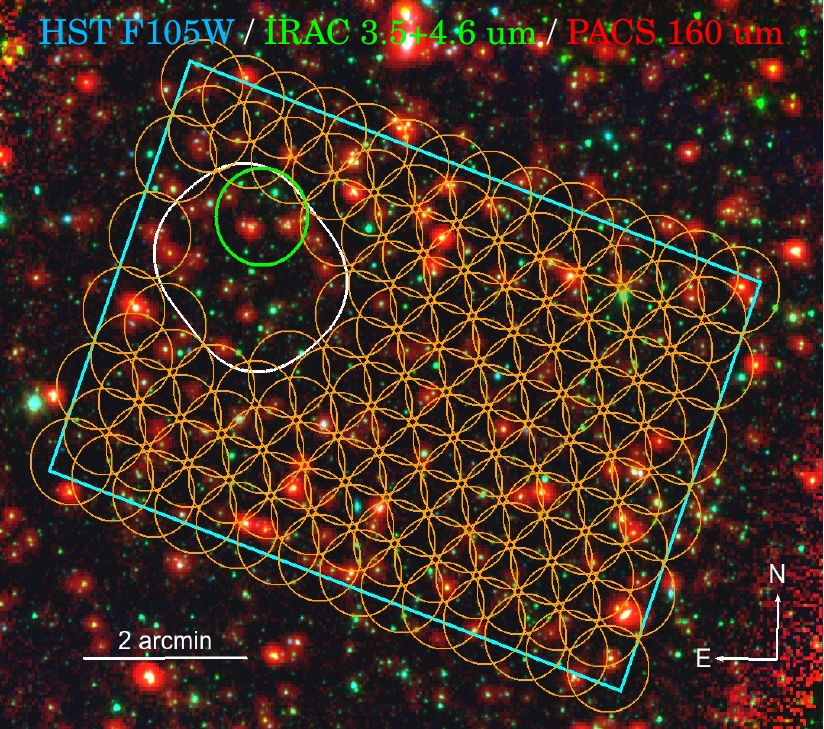
\includegraphics[width=120mm]{Wide_ASPECS_Coverage.png}
\caption{Spatial coverage of ASPECS Pilot (Green), Large Program (White), and Wide (Yellow) showing each of the individual pointings. The area covered by the Pilot is $~$1 arcmin$^2$, by the Large Program $~$5 arcmin$^2$, and by Wide ASPECS, $~$52.5 armin$^2$. The cyan box is the 50\% sensitivity extent of the survey. This region covers the area of the deepest CANDELS observations, where a wealth of ancillary data has been collected in over 30 photometric bands. Figure adapted from Decarli et al. (in prep.)} % Decarli in report
% Put this in the Wide ASPECS description stuff
\label{fig:ASPECS_Coverage}
\end{figure}

\begin{figure}[!htbp]
\centering
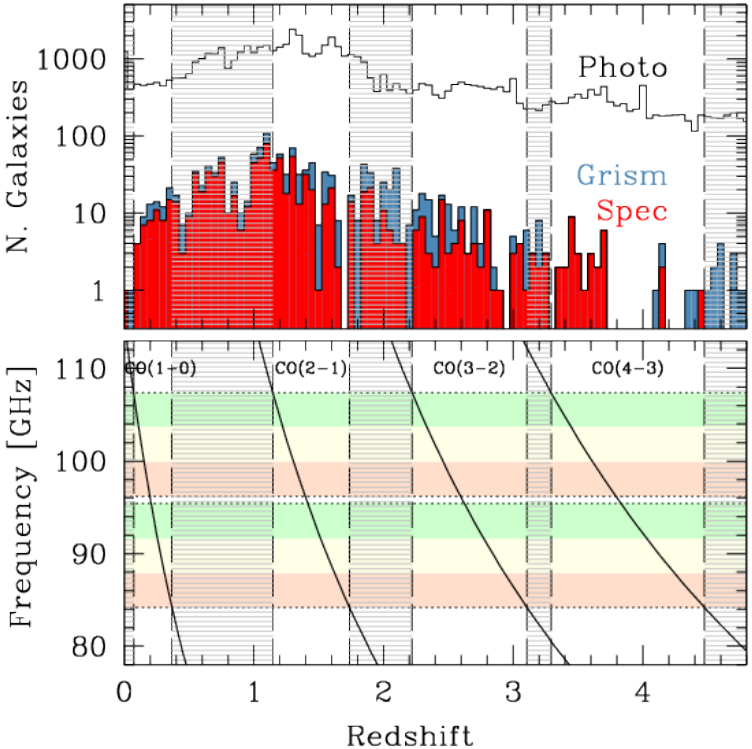
\includegraphics[width=120mm]{Wide_ASPECS_Freq.png}
\caption{Spectral and redshift coverage of Wide ASPECS in relation to the redshift distribution of galaxies within the survey field. Wide ASPECS is designed to detect CO line transitions at z$<$0.4, 1.1 $<$ z $<$ 1.8, and 2.2 $<$ z $<$ 4.4. Green, red, and yellow are the frequency ranges for A, B, and C frequency settings respectively. Figure adapted from Decarli et al. (in prep.)}
\label{fig:ASPECS_Freq}
\end{figure}

\begin{table}[!htb]
\caption{Redshift limits and cosmic volume probed for each CO transition observable by Wide ASPECS.}
\begin{tabular}{lllll}\label{table:CO_freq}
Transition & $z_{low}$ & $z_{high}$ & Freq. (GHz) & Volume (Mpc$^3$) \\
\hline
1-0        & 0.0030    & 0.3694     & 115.271     & 4461             \\
2-1        & 1.0059    & 1.7387     & 230.538     & 107411           \\
3-2        & 2.0088    & 3.1080     & 345.796     & 191232           \\
4-3        & 3.0115    & 4.4771     & 461.041     & 237143          
\end{tabular}
\end{table}

\subsection{Ancillary Data}\label{sec:ancillary}

In addition to each of the ALMA data cubes, there is a lot of ancillary data available as the GOODS-South region is one of the most studied regions of the sky. This data has been collected by combining multiple catalogs, first described in \cite{walter2016alma} and expanded with new data in \cite{decarli2019alma}, comprising over 30 photometric bands for over 63000 galaxies in and around the footprint of Wide ASPECS. 26251 galaxies lie within the footprint of Wide ASPECS, of which 2283 have spectroscopic redshifts, and 23968 have photometric redshifts. 

The majority of the ancillary data comes from the Hubble Space Telescope (HST) Cosmic Assembly Near-infrared Deep Extragalactic Legacy Survey (CANDELS)\cite{grogin2011candels, Koekemoer_2011}. Most of the photometric data comes from \cite{skelton20143d}, which additionally includes ground-based optical and NIR photometry from \cite{nonino2009deep, hildebrandt2006gabods, erben2005gabods, retzlaff2010great, Hsieh_2012, 2008ApJ...682..985W, cardamone2010multiwavelength}, as well as Spitzer IRAC 3.6$\mu$m, 4.5$\mu$m, 5.8$\mu$m, and 8.0$\mu$m photometry from \cite{dickinson2003evolution, elbaz2011goods, 2013ApJ...769...80A}. There is also photometric information from the Spitzer MIPS 24$\mu$m from \cite{Whitaker_2014}, and ALMA 1.1mm data from \cite{franco2018goods}. Additional far-infrared data from Herschel PACS at 100$\mu$m and 160$\mu$m as obtained from \cite{elbaz2011goods}. Spectroscopic redshifts came mostly from the MUSE Hubble Ultra Deep Survey \cite{bacon2017, inami2017} while more spectroscopic information was included from \cite{le2005vimos, coe2006galaxies, skelton20143d, morris2015wfc3}. Hubble grism spectroscopy was taken from the 3D-HST survey \cite{momcheva20163d}.

\subsection{Galaxy SED Fitting}

All observations of a galaxy recorded in gamma and X-rays, visible light, infrared, radio and UV give us part of the total spectral energy distribution (SED) of that galaxy. The more wavelengths a galaxy is measured in, the better constrained the SED, and the more complete our understanding of its energy distribution. Software, such as MAGPHYS \cite{da2008simple, da2015alma}, can use these observations to estimate a galaxy's physical parameters. These programs match the observed SED to precomputed models and output likelihood estimates for the properties of a given galaxy, such as the star-formation rate, mass, and dust temperature.

To estimate the properties of the galaxies in the catalog, the SED fitting program MAGPHYS was used \cite{da2008simple, da2015alma}. MAGPHYS computes a marginalized likelihood distribution for each of the different physical parameters of the observed galaxy through comparing the observed SED with the precomputed models. It also outputs the best-fit total SED for a given galaxy. In this report, the MAGPHYS high-z extension was used, which updates the original MAGPHYS with extended star-formation history and dust optical depth priors and adds intergalactic medium absorption in the ultraviolet \cite{da2015alma}.

An example output from MAGPHYS is shown in Fig. \ref{fig:MAGPHYS_Example}, displaying the model, the likelihood values for various physical properties of the galaxy, and the data points used to compute the SED in red. The distribution of the stellar mass, and star-formation rates of all the galaxies fitted with MAGPHYS are shown in Fig. \ref{fig:MAGPHYS_Mstar} and Fig. \ref{fig:MAGPHYS_SFR} respectively. Galaxies whose computed star-formation rate was at or below a $log_{10}(SFR) = -1.99$ were removed from the rest of the analysis, as this seemed to indicate a very poor MAGPHYS fit. That left a total of around 55000 galaxies in the sample, of which 22073 were in the Wide ASPECS footprint.

\begin{figure}[!hbp]
% Make Larger
\centering 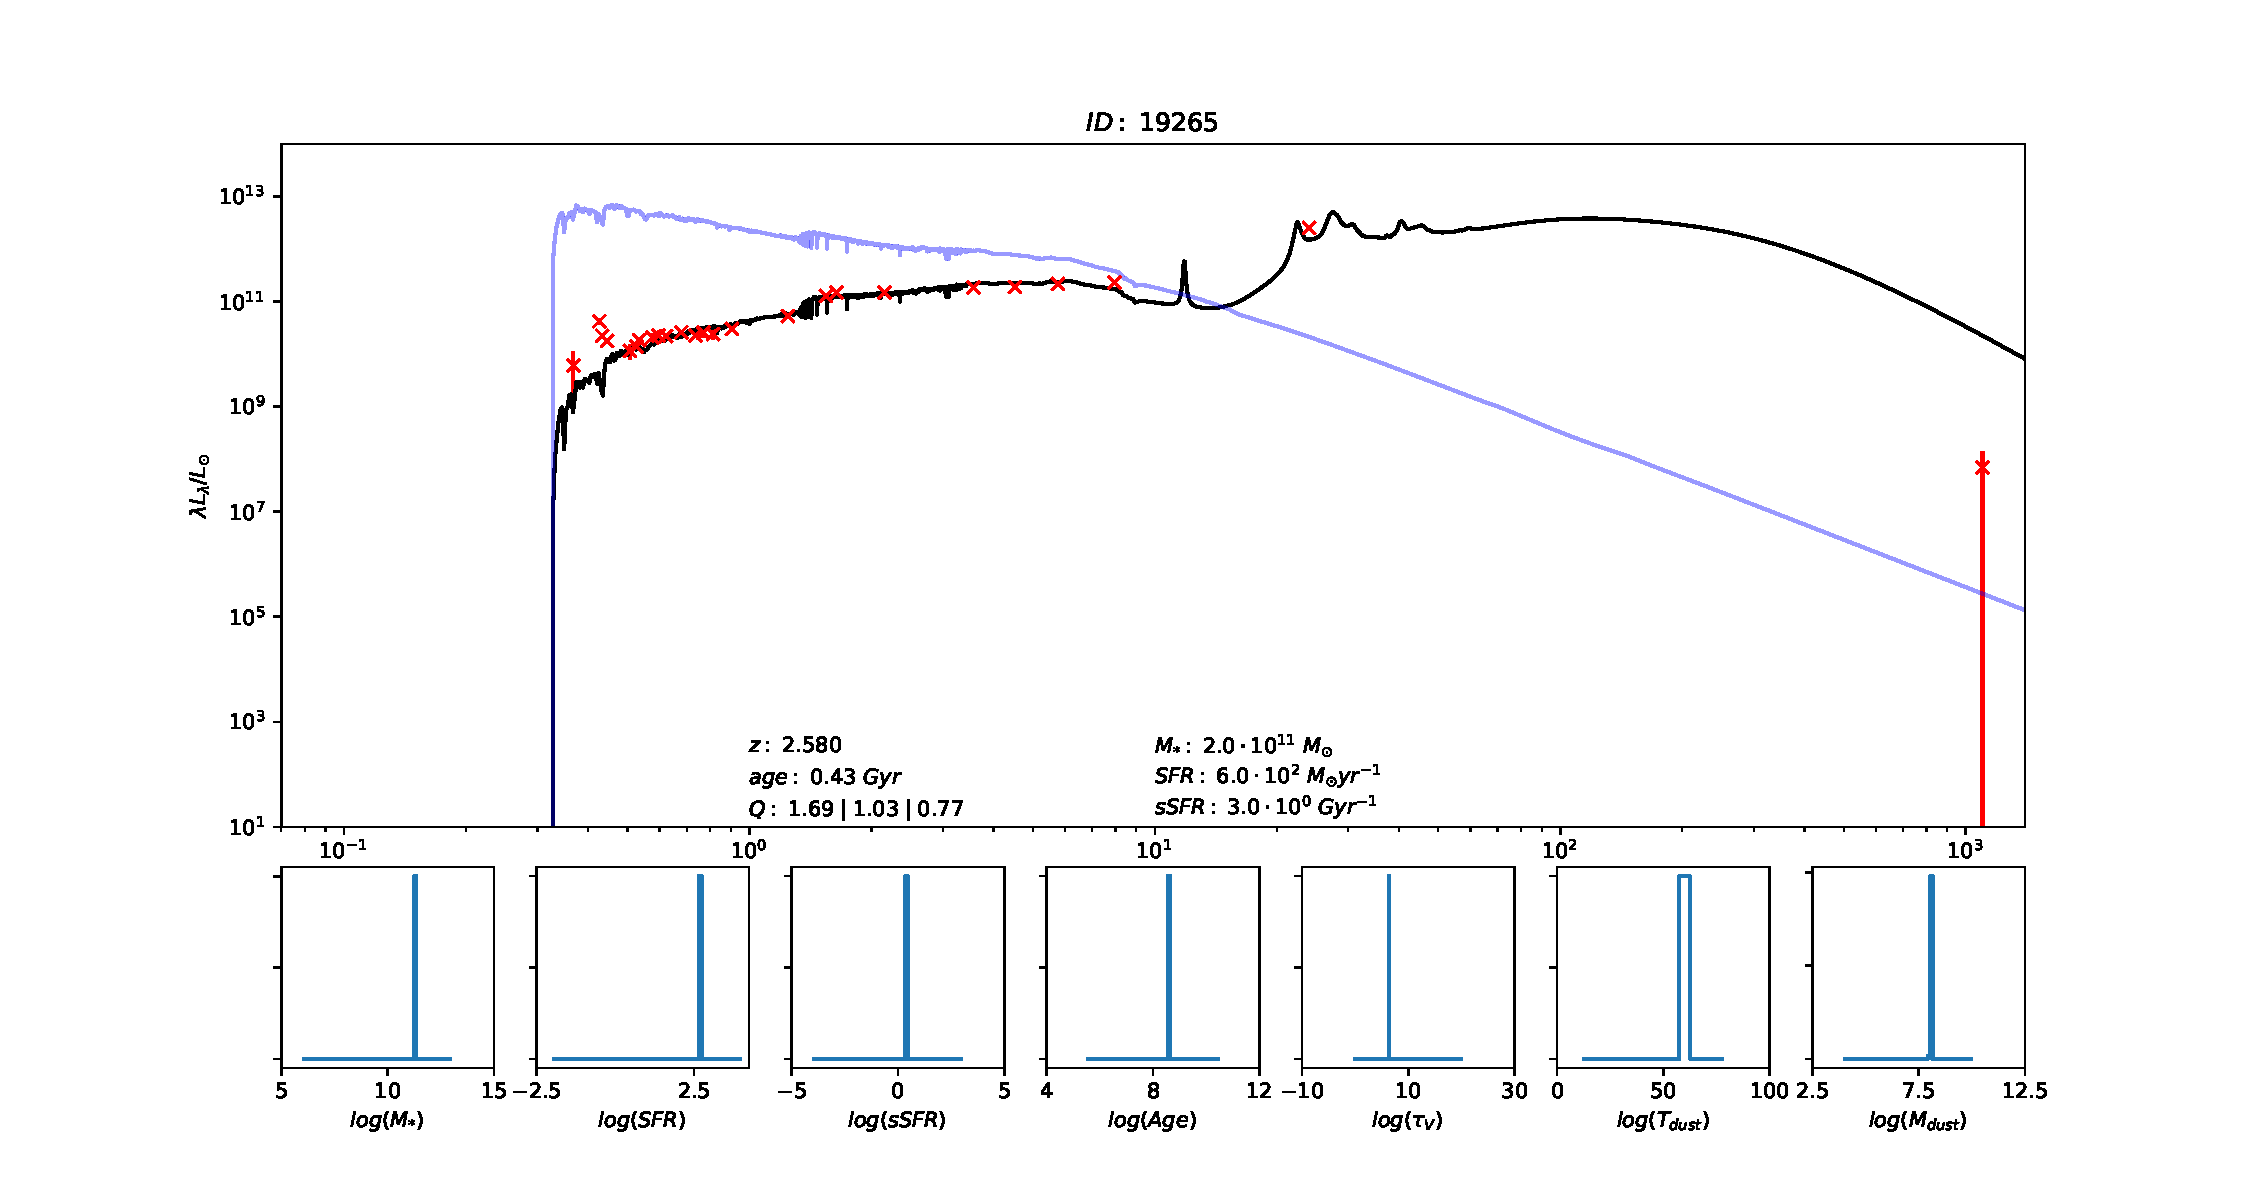
\includegraphics[width=160mm]{19265.pdf}
\caption{Example MAGPHYS output, from the most massive matched galaxy, ID.1 in Table \ref{table:Catalog}. The blue line is the spectrum of the galaxy without attenuation. The black line is the model used by MAGPHYS. The red dots are the data points. The bottom row of graphs show the probability distribution for various physical properties.}
\label{fig:MAGPHYS_Example}
\end{figure}

\begin{figure}[!htbp]
\centering 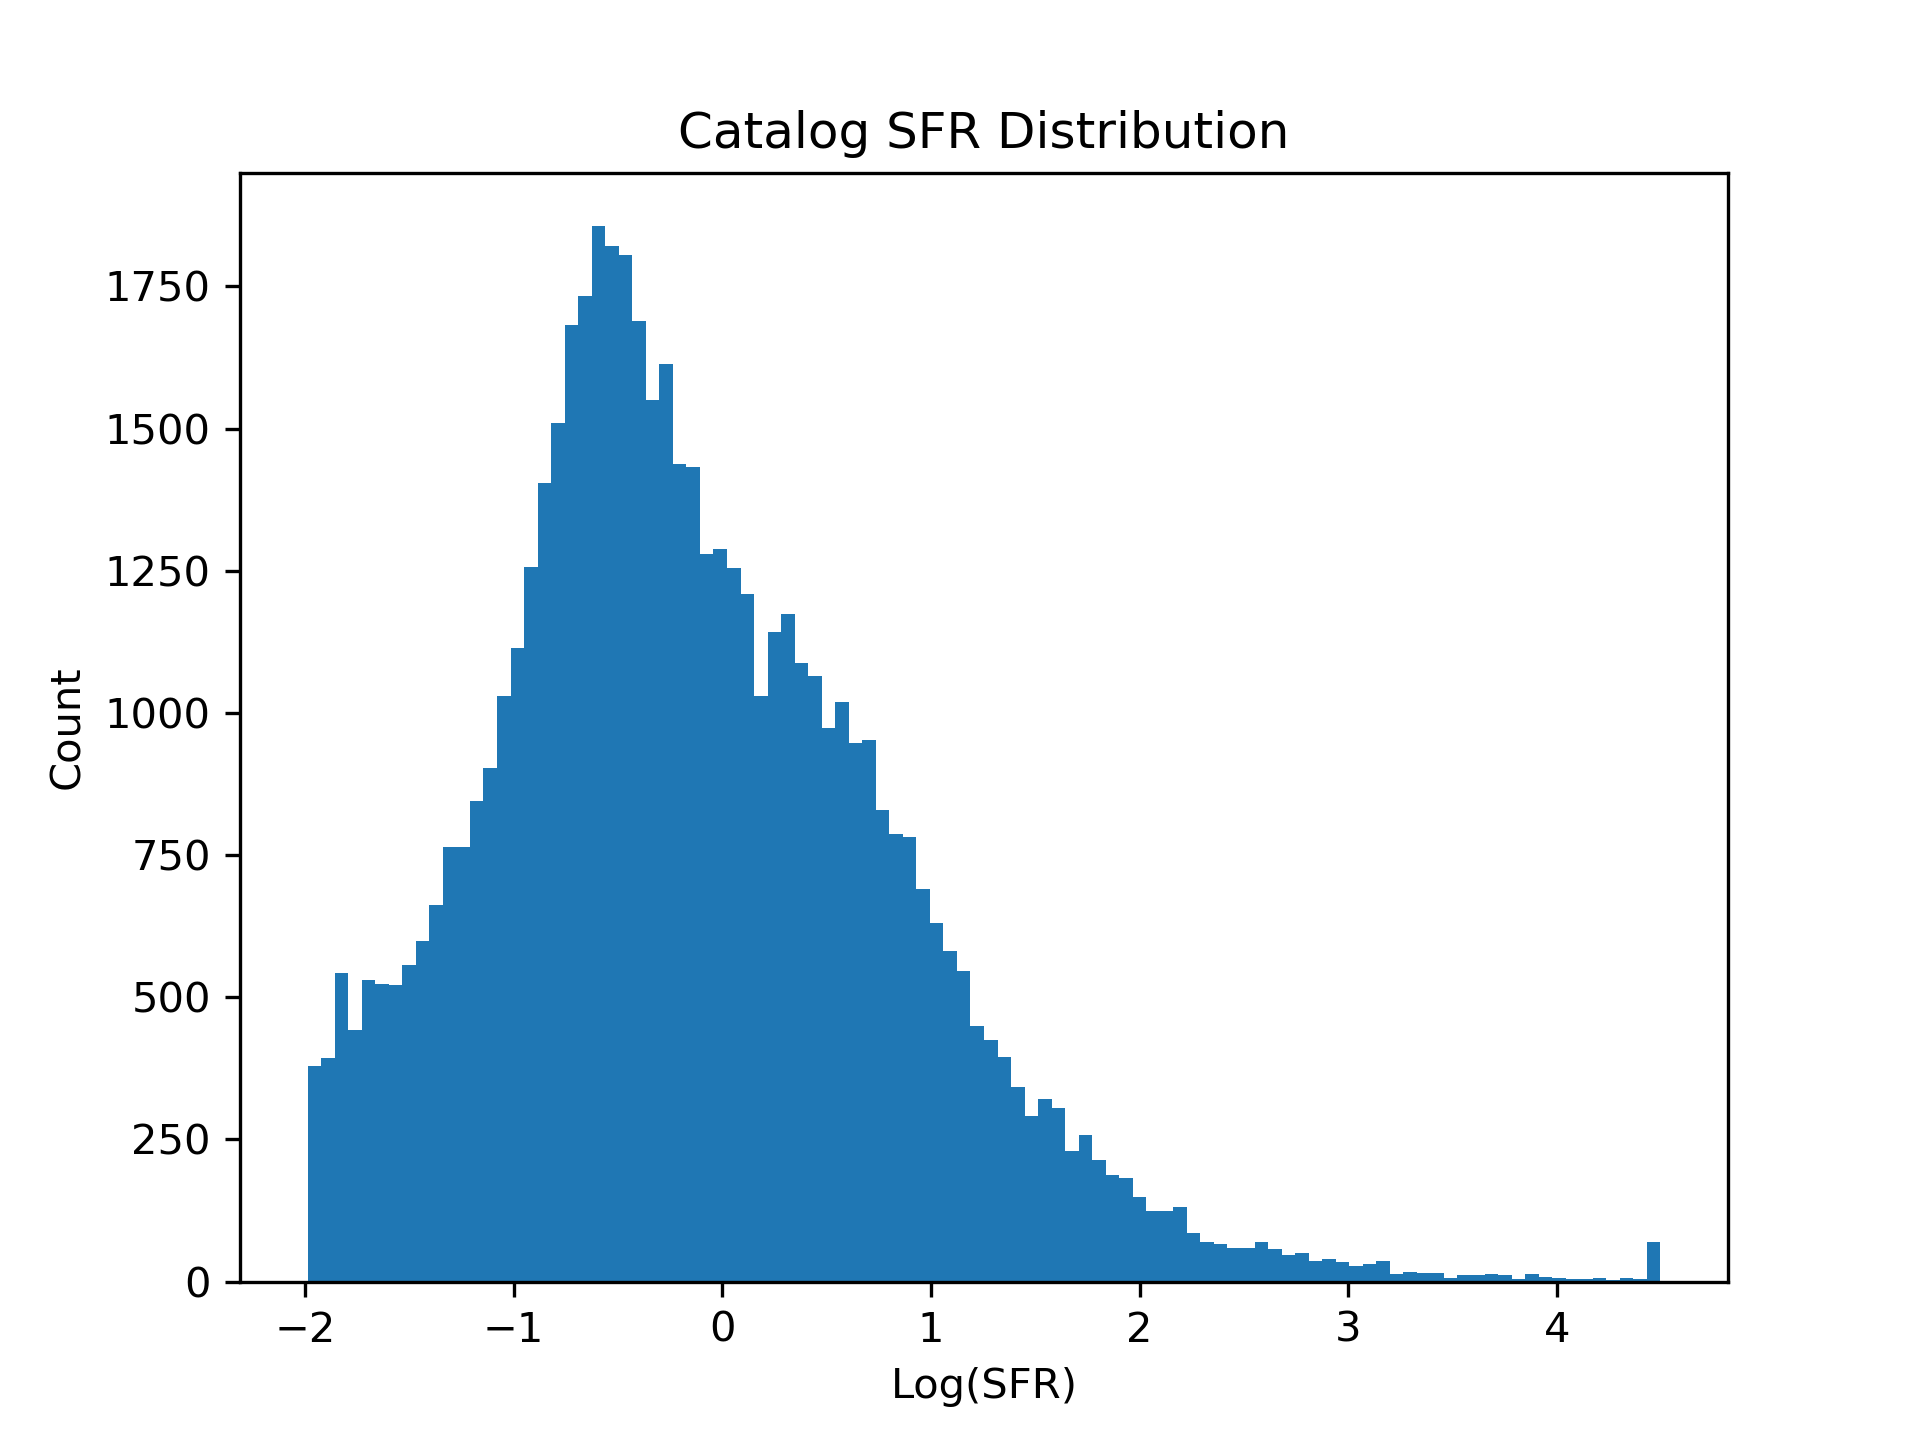
\includegraphics[width=87mm]{Survey/MAGPHYS_SFR.png}
\caption{Distribution of star-formation rate for all galaxies in the catalog. The cutoff at -1.99 is from the quality cut to remove galaxies that had very poor MAGPHYS fits.}
\label{fig:MAGPHYS_SFR}
\end{figure}

\begin{figure}[!htbp]
\centering 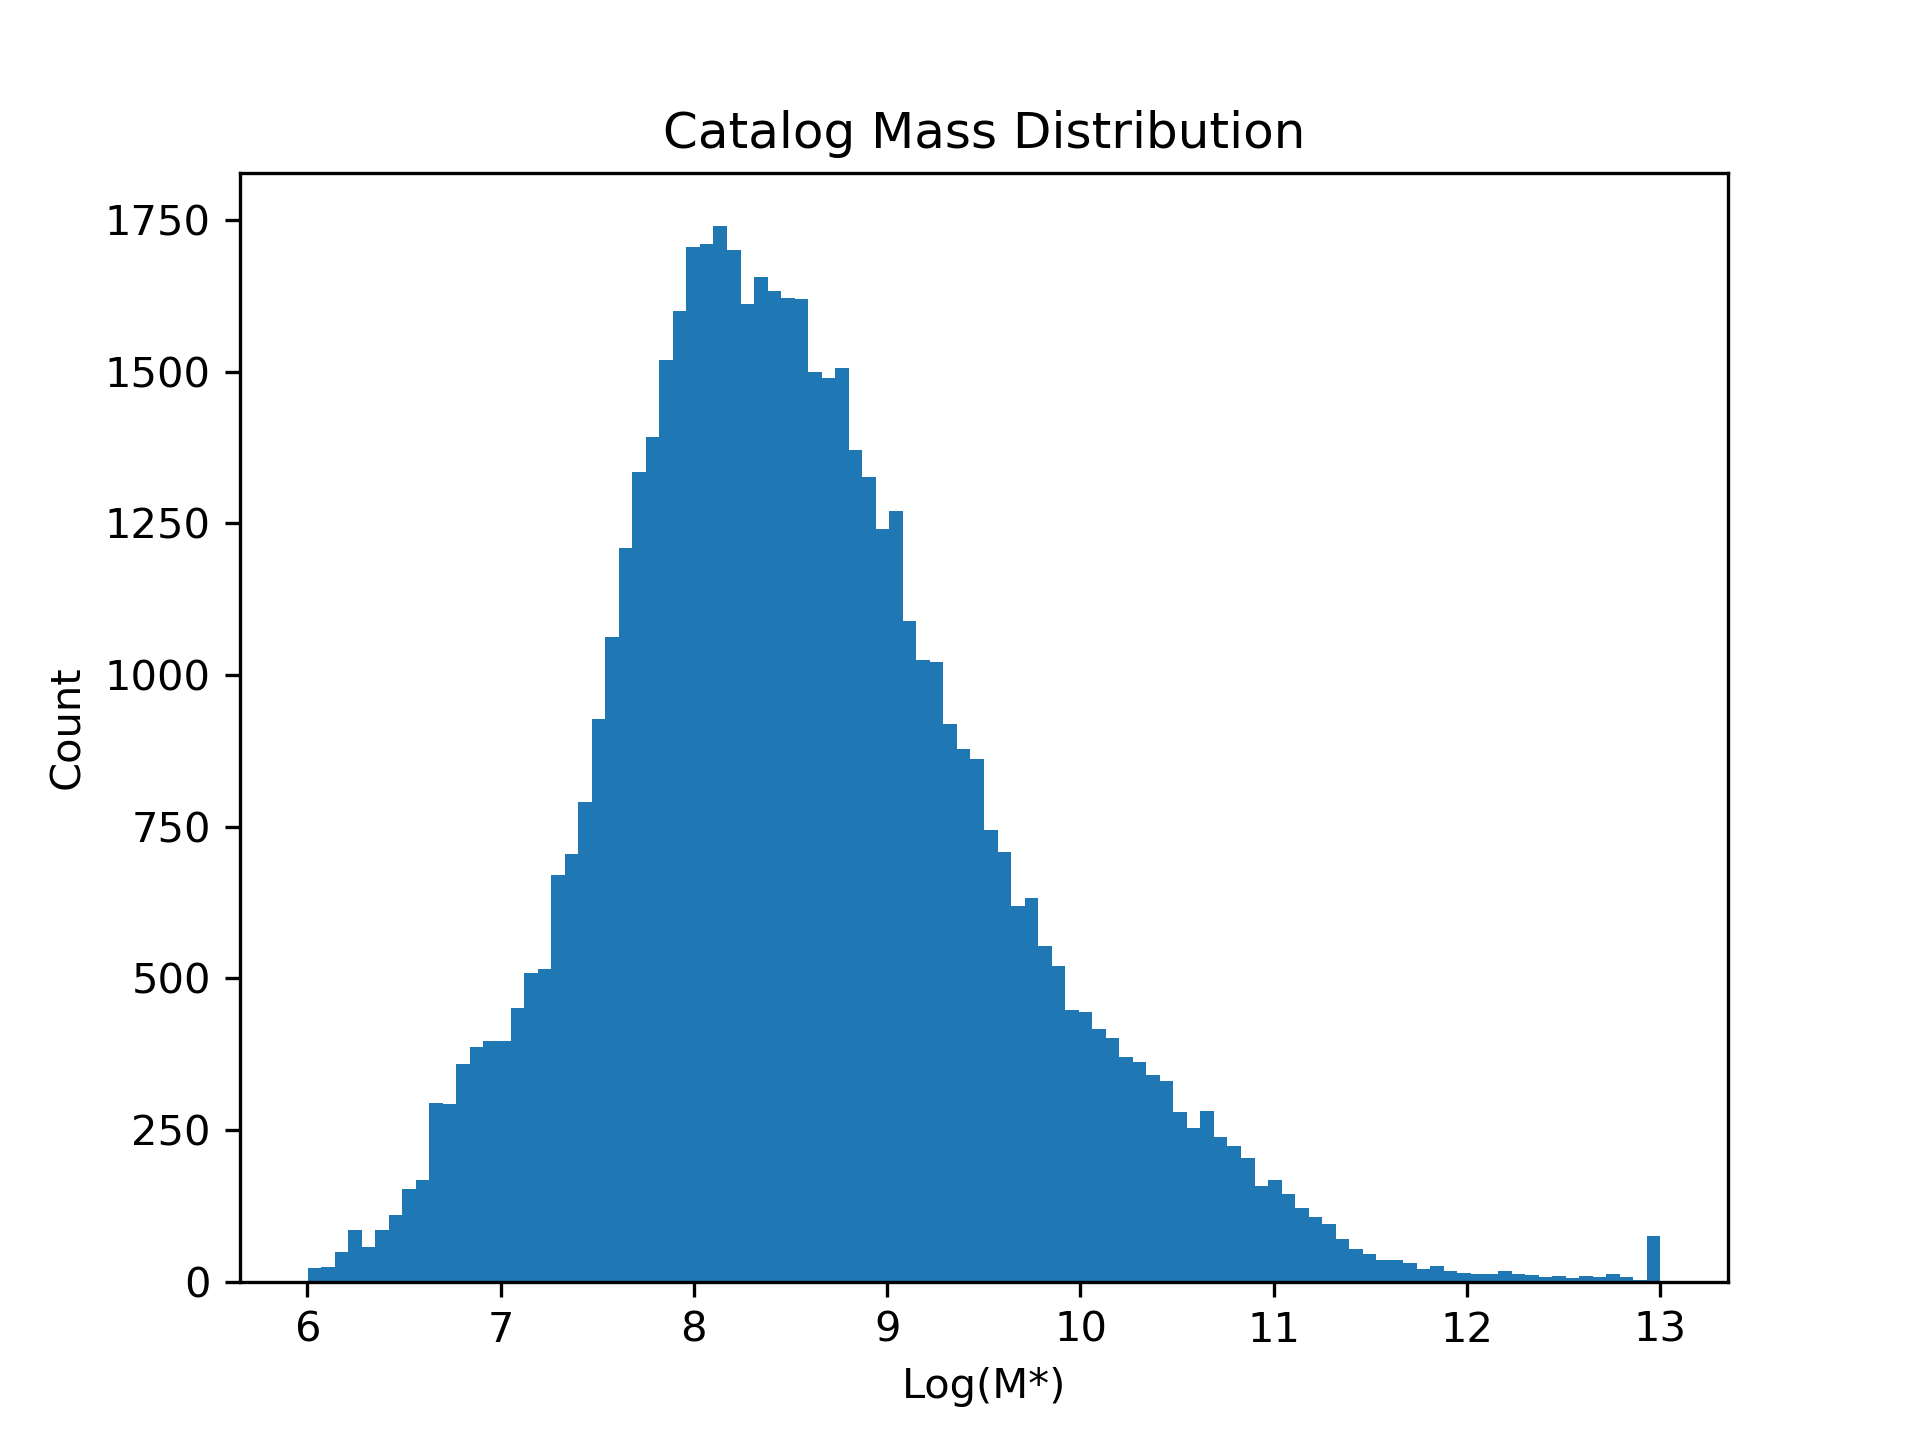
\includegraphics[width=87mm]{Survey/MAGPHYS_Mstar.png}
\caption{Distribution of stellar mass for all galaxies in the catalog. These galaxies have undergone the same quality cut as for the star-formation rate plot.}
\label{fig:MAGPHYS_Mstar}
\end{figure}

\section{The CO Emission Line Catalog}

The method for finding CO emission lines in the ALMA data cubes, computing the fidelity of the lines, cross-matching the CO emitter candidates with the galaxy catalog, and determining matches is the same process as used in the other ASPECS surveys \cite{walter2016alma, decarli2019alma, gonzalez2019alma}.

\subsection{Line Search and Fidelity}

To find possible CO emitters, a search for CO lines was done with the FindClump algorithm first described in \cite{walter2016alma}. This code searches along the spectral axis with different kernel widths in order to maximize the sensitivity to signals associated with line candidates of different intrinsic widths. The widths range from 3 spectral channels up to 19 channels, with each channel being 7.813 MHz wide, corresponding to widths of between 73.2 Km s$^{-1}$ to 463.6 Km s$^{-1}$ at 96 GHz. The data cubes are searched for lines at any spatial position and spectral coordinate, without any prior based on data from other wavelengths. This is done to minimize any bias in the selection. FindClump returns a list of potential line candidates that then have duplicates removed, which is done by grouping line candidates based on their spatial and spectral position in the cube from each group, only storing the candidate with the highest S/N \cite{walter2016alma}. This results in 11941 candidates at S/N$>$5.0, 1096 at S/N$>$5.5, 78 at S/N$>$6.0, and 6 at S/N$>$6.5. 

To get a sense of how many of these line candidates are false positives, the fidelity of the lines is then computed. To obtain the fidelity, a line search on the negative data cubes is performed using exactly the same algorithm as that used to detect lines in the positive data cubes. The negative cubes are obtained by multiplying all the values in each data cube by -1, and rerunning the line search. This catalog of negative lines is then used to compute the fidelity. The fidelity of a line at a given S/N is defined as 

$$ fideltiy(S/N) = 1 - \frac{N_{neg}(S/N)}{N_{pos}(S/N)} $$ where $N_{pos}(S/N)$ and $N_{neg}(S/N)$ are the number of positive and negative line candidates detected at that S/N and for a given line width, respectively \cite{gonzalez2019alma}.

The fidelity of the different line widths is shown in Fig. \ref{fig:Fid_map}. As can be seen, the fidelity of the lines is generally lower for narrower line widths as more independent resolution elements yield a larger probability of finding a few, high-S/N noise peaks in the cubes \cite{decarli2019alma}. The CO emission line catalog contains 16 lines at a fidelity $>$0.8, 20 at $>$0.7, 35 at $>$ 0.6, 52 at $>$ 0.5, and 69 at $>$ 0.4, and 81372 below a fidelity of 0.4. The fidelity cut used for the rest of this analysis is set at 0.6, where every given line has a 60\% chance of being a real line, and leaving us with 35 line candidates, which are listed in Table \ref{table:Catalog}.

\begin{figure}[!htbp]
\centering 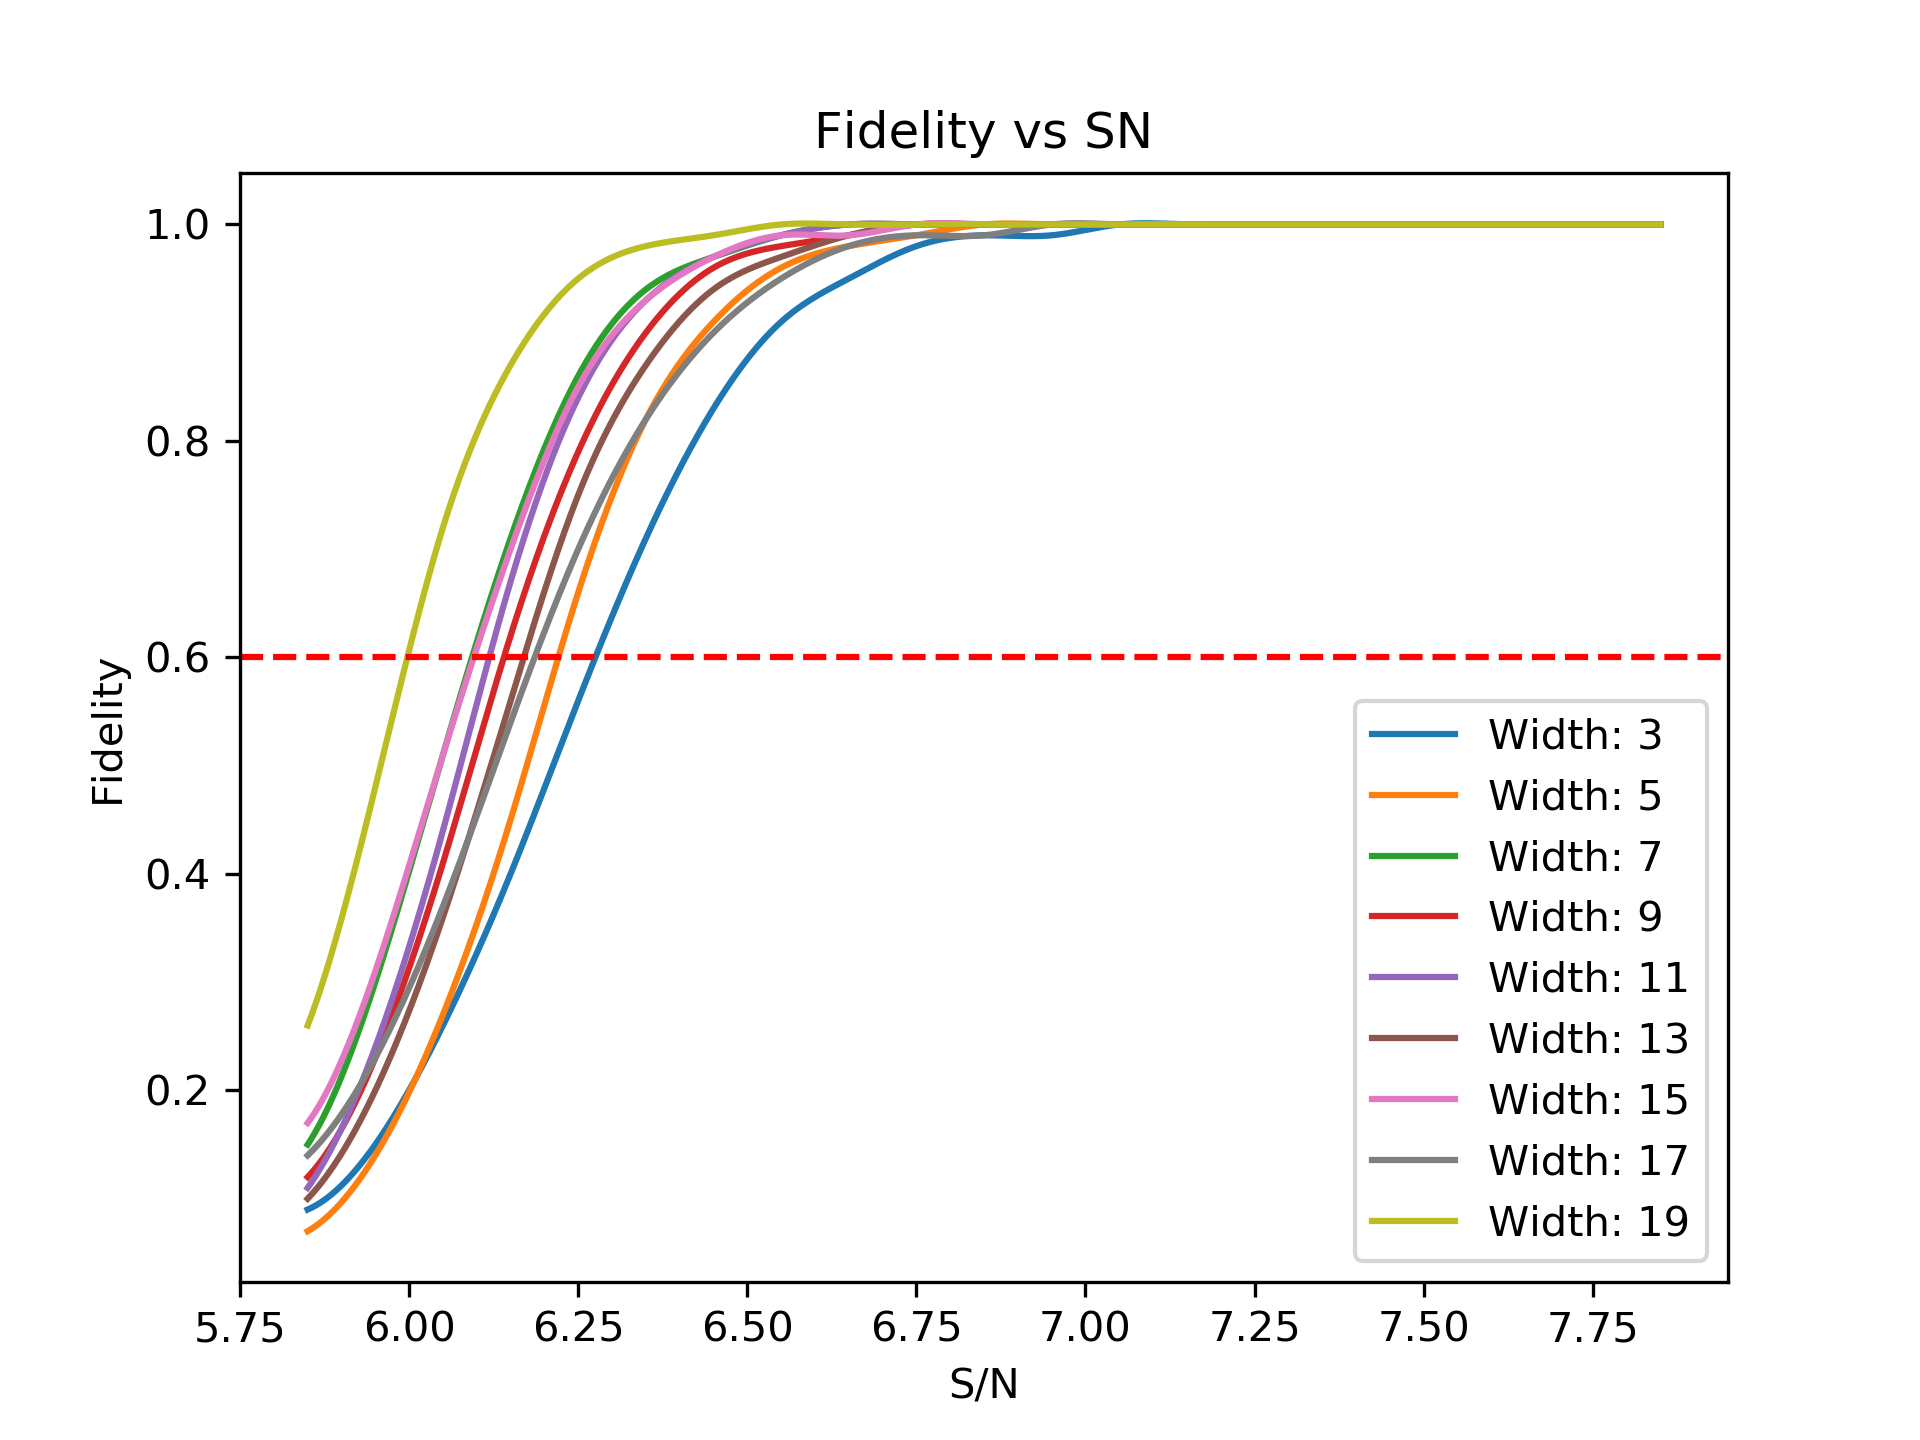
\includegraphics[width=120mm]{Fidelity_map.png}
\caption{Fidelity vs S/N for the different line widths used by FindClump. The red dotted line shows the fidelity = 0.6 cutoff used for the analysis in this report. There are a total of 35 line candidates above that cutoff.}
\label{fig:Fid_map}
\end{figure}

\subsection{Determination of the Redshift of the CO Emitters and Cross-matching with the Galaxy Catalog}

To determine the redshift of the CO emitters, we need to know the transition of the observed CO line. As shown in Table \ref{table:CO_freq}, there are multiple CO transitions which are spaced out almost equi-distant in frequency, with the CO(1-0), CO(2-1), CO(3-2), and CO(4-3) transitions having rest-frame frequencies of $\sim$115 GHz, $\sim$230 GHz, $\sim$345 GHz, and $\sim$460 GHz, respectively. This makes it difficult to determine the unique redshift for a given candidate, as multiple CO transitions could create the detected signal.

To determine the transition, and therefore the redshift, the next step after performing the line search and fidelity cut is to cross-match the CO lines to already known galaxies within the Wide ASPECS footprint. To do this, the spatial location of the line candidates is matched to galaxies that are within one arcsecond of the line candidate's location. Then, assuming that the CO line is from that matched galaxy, the CO transition is calculated. The match is only kept if the offset between the CO line's redshift and the galaxy's redshift, $\delta z$, is $|\delta z| < 0.01$ for galaxies with spectroscopic redshifts, or $|\delta z| < 0.3$ for ones with photometric redshifts. The differences in $|\delta z|$ thresholds are because spectroscopic redshifts are much more reliable and precise than photometric redshifts. 

If a line matches to more than a single galaxy then the following steps are performed to determine to which galaxy the line should be matched. The first step is to calculate the CO transition for the line assuming the line is matched to each of the galaxies. Then difference between the CO redshift and the galaxy's redshift is computed. The matched galaxy that gives the smallest $|\delta z|$ and whose redshift falls within the limits of Wide ASPECS is then saved as the matched galaxy for that line candidate. 

These counterparts provide information about the physical parameters of the line candidate. A summary of the line candidate counterparts for the fidelity $>$0.6 catalog is shown in Table \ref{table:matched_gal}. Cutouts of the three line candidates and their counterparts are shown in Figures \ref{fig:Count_One}, \ref{fig:Count_Five}, and \ref{fig:Count_Nine}. Of the counterparts, only ID.1's match has a spectroscopic redshift.

\begin{figure}[!htbp]
\centering 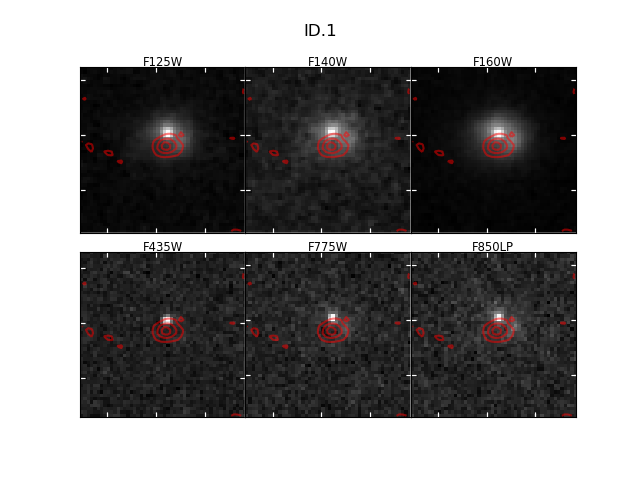
\includegraphics[width=100mm]{Matched/ASPECS_Cutout_0.png}
\caption{ID.1. Red contours signify +2$\sigma$,4$\sigma$,6$\sigma$,and 8$\sigma$. The size of the cutouts are 3x3 arcseconds. The spacing between the ticks is one arcsecond.}
\label{fig:Count_One}
\end{figure}

\begin{figure}[!htbp]
\centering 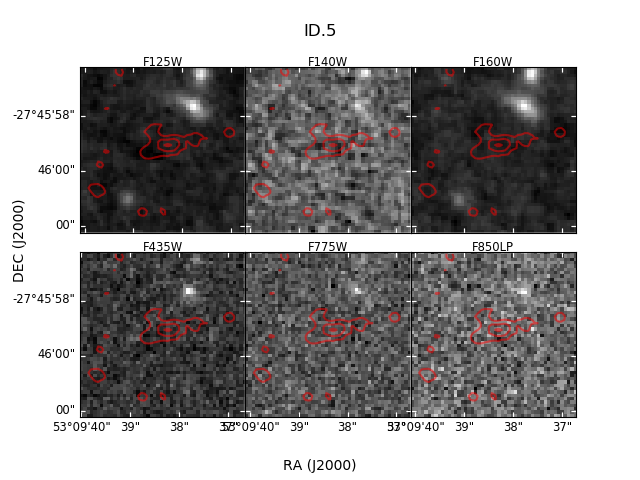
\includegraphics[width=100mm]{Matched/ASPECS_Cutout_4.png}
\caption{ID.5. Same contours and size as for Fig. \ref{fig:Count_One}. }
\label{fig:Count_Five}
\end{figure}

\begin{figure}[!htbp]
\centering 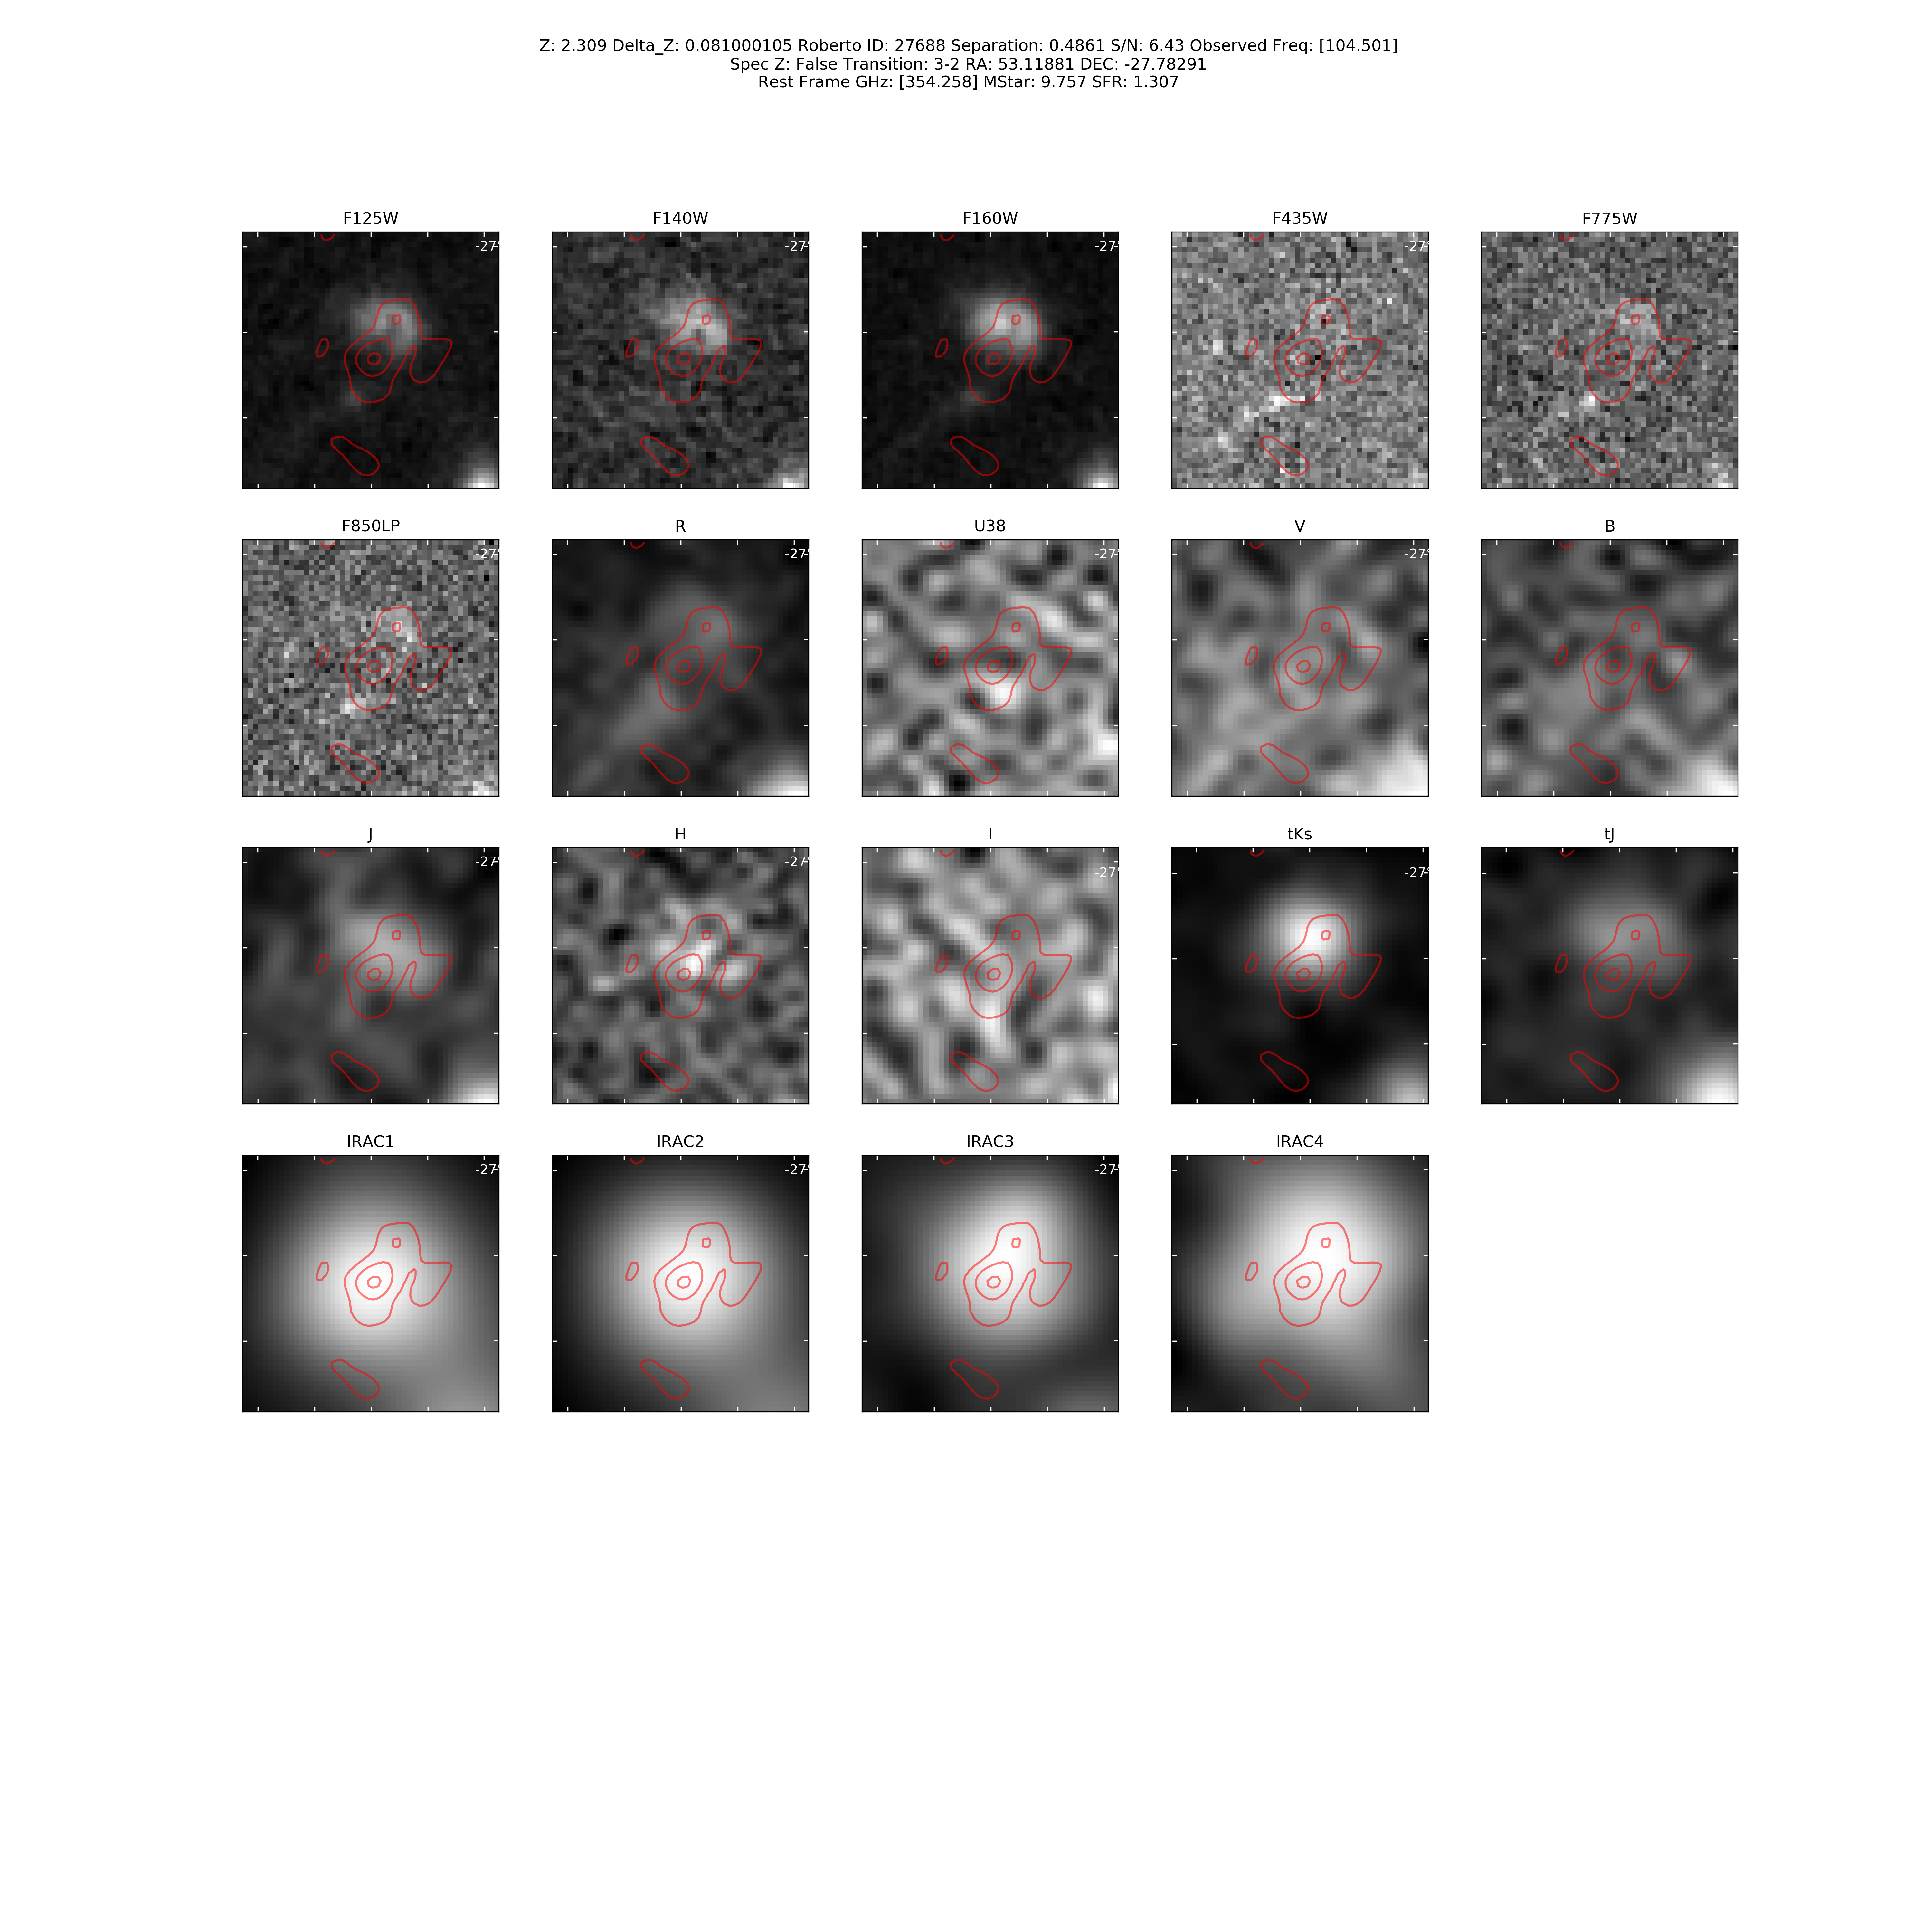
\includegraphics[width=100mm]{Matched/ASPECS_Cutout_8.png}
\caption{ID.9. Same contours and size as for Fig. \ref{fig:Count_One}.}
\label{fig:Count_Nine}
\end{figure}

If there is not a match to a galaxy in the catalog, or if the galaxy's redshift is incompatible with the CO line identification then the line identification is performed by a bootstrap method. As seen in Table \ref{table:CO_freq}, each CO transition is detectable within a certain redshift range, and that redshift range determines the volume sampled at each transition. The larger the cosmic volume probed by a given transition the more likely that an unidentified line is that transition, where the probability of a line candidate being one of CO(1-0), CO(2-1), CO(3-2), or CO(4-3) is proportional to the volume of the universe sampled in each of those transitions \cite{walter2016alma, decarli2019alma}. Once the CO line candidate's transition is determined, the redshift is computed through $ z_{CO} = \frac{Restframe_{freq}}{Obs_{freq}} - 1 $. The results of the line matching for the fidelity $>$ 0.6 sample are shown in Table \ref{table:Catalog}, and the redshift distribution of the line candidates is shown in Fig. \ref{fig:cat_red}.

\begin{table}[!htbp]
\centering
\caption{The 35 CO line candidates from the fidelity $>$ 0.6 cut.}
\begin{tabular}{ccccccccc}
ID\tablefootnote{Assigned ID for the candidate} & RA\tablefootnote{J2000 system (degrees)} & DEC\tablefootnote{J2000 system (degrees)} & $v_{CO}$\tablefootnote{Observed frequency of the source in GHz.} & CO Tran.\tablefootnote{Estimated CO transition for the line candidate. Goes from $J_{up}$ to $J_{lower}$, e.g. 3-2 is the CO(3-2) transition.} & $z_{CO}$\tablefootnote{Redshift as determined by the CO transition.} & $\delta z$\tablefootnote{Difference in redshift between the CO line transition and the galaxy the line is matched to, if there is one.} & S/N\tablefootnote{Signal-to-noise of the CO line.}& Match?\tablefootnote{If there is a match between the CO line and the galaxy catalog.} \\
\hline
ID.1 & 53.14886 & -27.82118 & 96.701 & 3-2 & 2.576 & 0.006 & 7.31 & Y \\
ID.2 & 53.19145 & -27.76985 & 91.657 & 2-1 & 1.515 & -- & 6.82 & N \\
ID.3 & 53.14138 & -27.84409 & 96.834 & 4-3 & 3.761 & -- & 6.72 & N \\
ID.4 & 53.19242 & -27.78342 & 106.72 & 3-2 & 2.24 & -- & 6.63 & N \\
ID.5 & 53.16066 & -27.76629 & 86.677 & 2-1 & 1.66 & -0.237 & 6.6 & Y \\
ID.6 & 53.16003 & -27.76258 & 103.36 & 3-2 & 2.346 & -- & 6.6 & N \\
ID.7 & 53.13447 & -27.74976 & 102.719 & 3-2 & 2.366 & -- & 6.49 & N \\
ID.8 & 53.11066 & -27.82727 & 85.654 & 3-2 & 3.037 & -- & 6.45 & N \\
ID.9 & 53.11881 & -27.78291 & 104.501 & 3-2 & 2.309 & 0.081 & 6.43 & Y \\
ID.10 & 53.13921 & -27.75352 & 86.67 & 3-2 & 2.99 & -- & 6.43 & N \\
ID.11 & 53.07696 & -27.8251 & 90.891 & 2-1 & 1.536 & -- & 6.42 & N \\
ID.12 & 53.12766 & -27.76666 & 99.553 & 4-3 & 3.631 & -- & 6.42 & N \\
ID.13 & 53.07796 & -27.80182 & 98.725 & 4-3 & 3.67 & -- & 6.36 & N \\
ID.14 & 53.13923 & -27.78228 & 94.407 & 2-1 & 1.442 & -- & 6.35 & N \\
ID.15 & 53.04266 & -27.79322 & 103.173 & 3-2 & 2.352 & -- & 6.3 & N \\
ID.16 & 53.116 & -27.84624 & 97.569 & 4-3 & 3.725 & -- & 6.29 & N \\
ID.17 & 53.09146 & -27.8497 & 106.235 & 3-2 & 2.255 & -- & 6.27 & N \\
ID.18 & 53.18748 & -27.81369 & 89.704 & 1-0 & 0.285 & -- & 6.27 & N \\
ID.19 & 53.11238 & -27.75628 & 88.735 & 3-2 & 2.897 & -- & 6.26 & N \\
ID.20 & 53.12915 & -27.79241 & 91.54 & 2-1 & 1.518 & -- & 6.22 & N \\
ID.21 & 53.1179 & -27.8184 & 92.876 & 2-1 & 1.482 & -- & 6.21 & N \\
ID.22 & 53.06549 & -27.84266 & 104.094 & 3-2 & 2.322 & -- & 6.21 & N \\
ID.23 & 53.1612 & -27.76049 & 94.618 & 2-1 & 1.437 & -- & 6.19 & N \\
ID.24 & 53.11182 & -27.82032 & 99.522 & 4-3 & 3.633 & -- & 6.19 & N \\
ID.25 & 53.07121 & -27.82724 & 88.954 & 3-2 & 2.887 & -- & 6.17 & N \\
ID.26 & 53.19977 & -27.8282 & 100.055 & 3-2 & 2.456 & -- & 6.16 & N \\
ID.27 & 53.06316 & -27.82356 & 84.623 & 3-2 & 3.086 & -- & 6.15 & N \\
ID.28 & 53.09788 & -27.76003 & 90.618 & 3-2 & 2.816 & -- & 6.13 & N \\
ID.29 & 53.16282 & -27.84445 & 90.571 & 3-2 & 2.818 & -- & 6.12 & N \\
ID.30 & 53.09665 & -27.81229 & 95.259 & 2-1 & 1.42 & -- & 6.12 & N \\
ID.31 & 53.13844 & -27.80491 & 102.376 & 3-2 & 2.378 & -- & 6.12 & N \\
ID.32 & 53.16516 & -27.82257 & 104.931 & 3-2 & 2.295 & -- & 6.11 & N \\
ID.33 & 53.19483 & -27.81481 & 98.873 & 4-3 & 3.663 & -- & 6.1 & N \\
ID.34 & 53.08948 & -27.78102 & 86.068 & 3-2 & 3.018 & -- & 6.1 & N \\
ID.35 & 53.14828 & -27.84444 & 87.302 & 3-2 & 2.961 & -- & 6.1 & N \\
\end{tabular}
\end{table}\label{table:Catalog}

\section{Physical Properties of the CO emitters}

The stellar mass versus star-formation rate is shown for the general galactic population and the 3 ASPECS counterparts in Fig. \ref{fig:Cross_match}. For comparison, the Schreiber et al. 2015 \cite{schreiber2015herschel} (as S15) and Whitaker et al. 2014 \cite{Whitaker_2014} (as W14) main sequence fits are plotted as well. As can be seen, two of the matched galaxies are above the main sequence and are massive, star-forming galaxies that are the expected type of galaxies for this survey to match to. The other galaxy is much less massive than expected. 

\begin{figure}[!htbp]
\centering 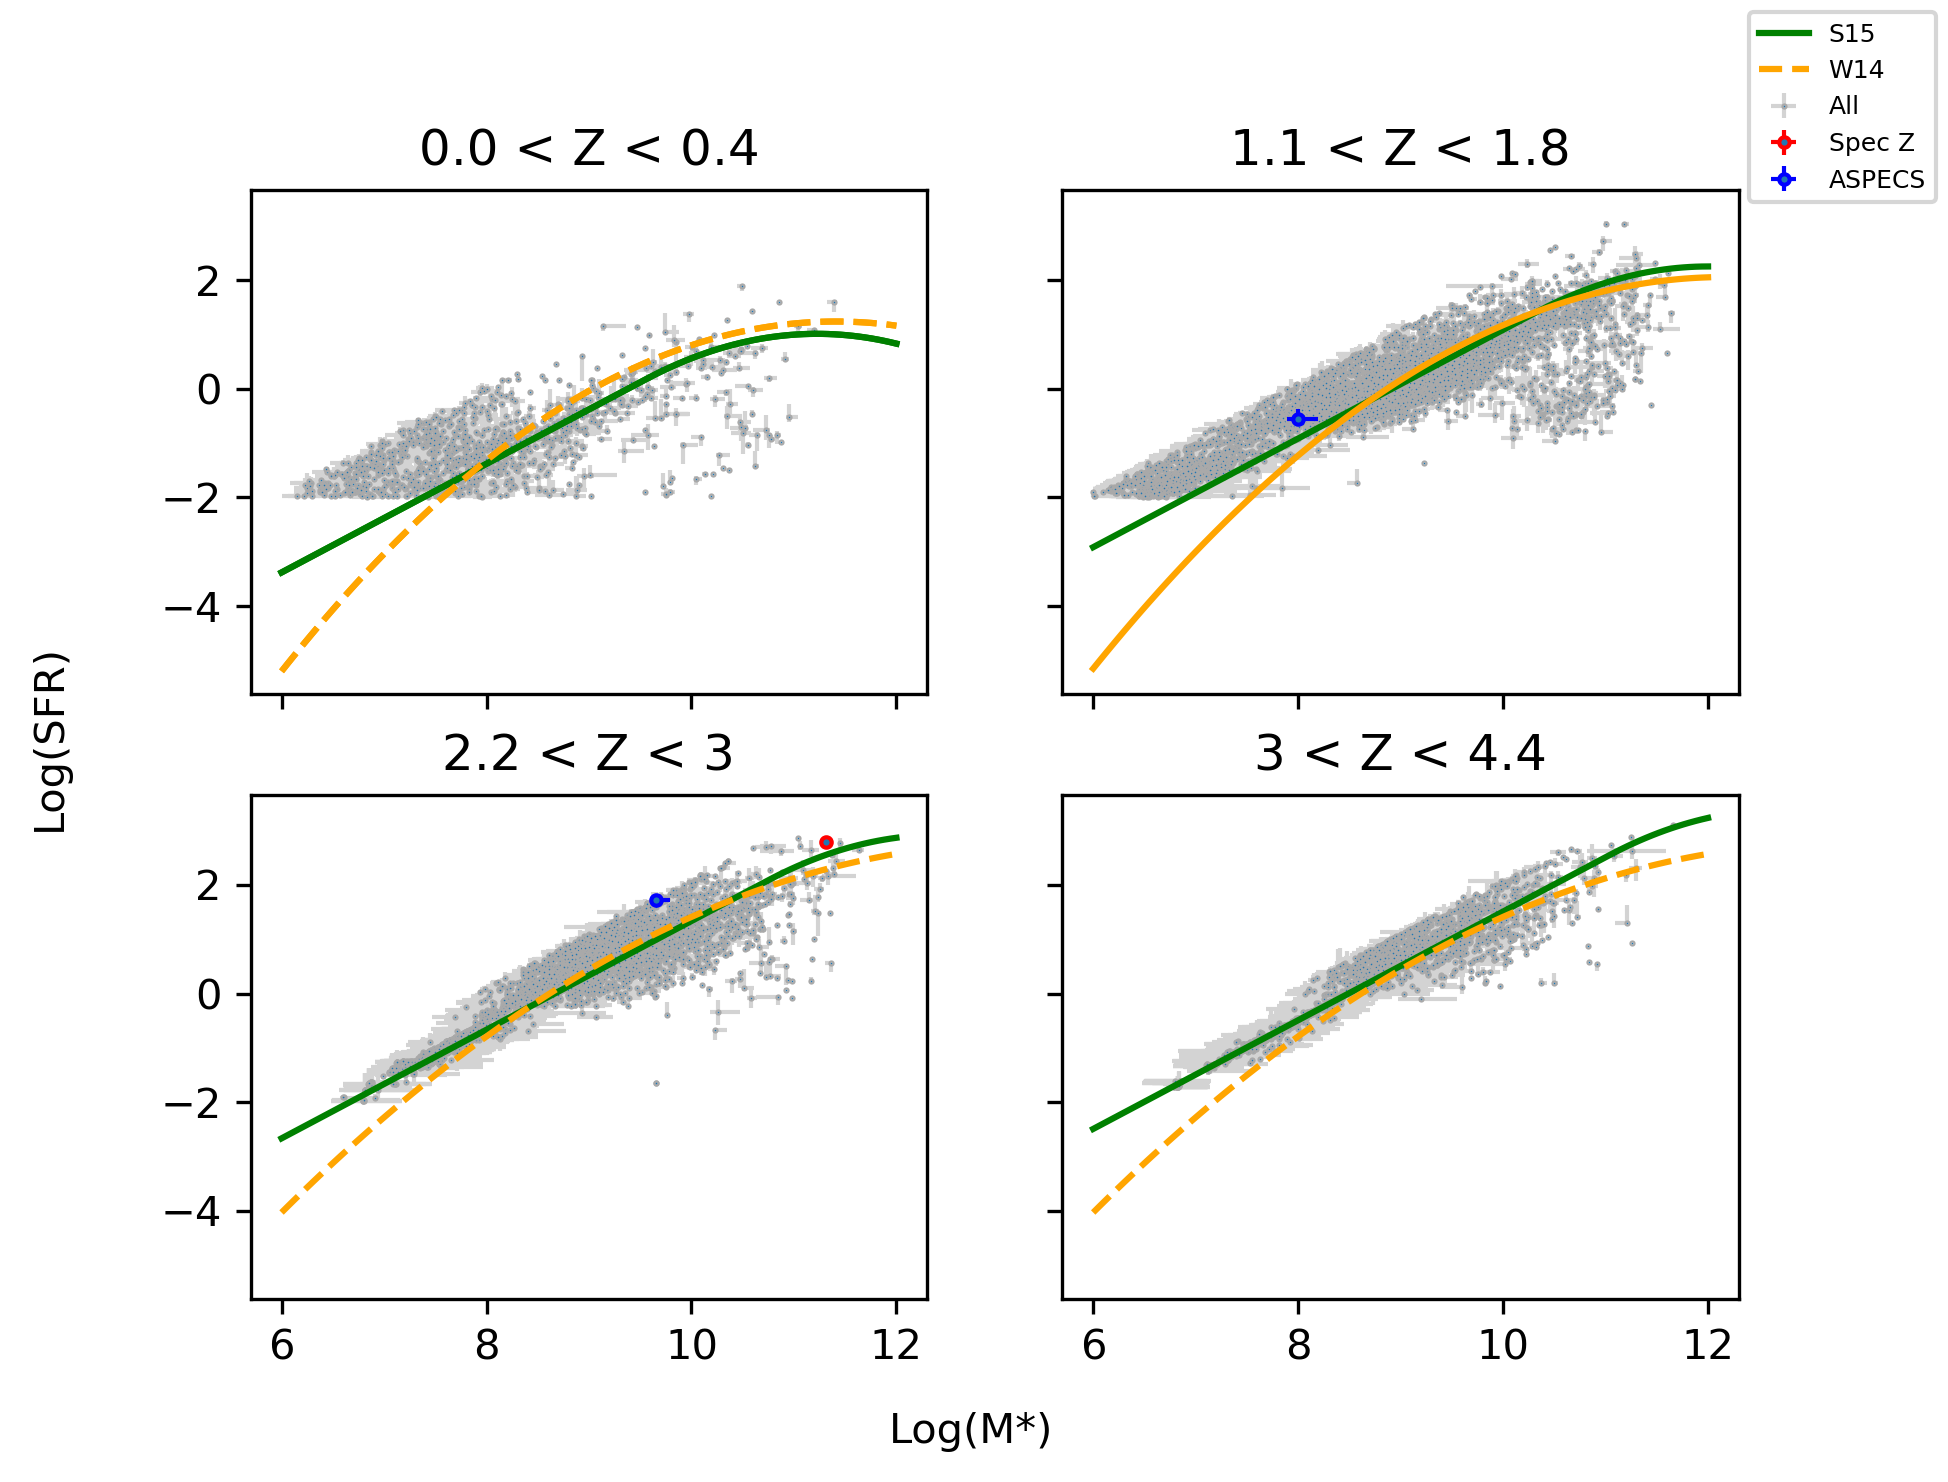
\includegraphics[width=120mm]{Survey/No_Cut_Mstar_vs_SFR_all_closest_sep_1_0_sn_fid_60.png}
\caption{Stellar mass versus star-formation rate for galaxies that the fidelity $>$ 0.6 CO line sample matched to. Red points are matched galaxies with spectroscopic redshifts, while blue points are matched galaxies with photometric redshifts. Grey points are all the galaxies in the compiled catalog from \ref{sec:ancillary}. The green lines are the galaxy main sequence fits from \cite{schreiber2015herschel}. The yellow line is from \cite{Whitaker_2014}'s galactic main sequence fit, where the solid line means it is computed within the range mentioned in the paper, while dotted means that the values are extrapolated from the paper to higher, or lower, redshifts. Two of the three matches are on the upper edge of the main sequence, while the third match has a much lower stellar mass and star-formation rate than expected for this survey. Error bars are the 16/84th percentile outputs from MAGPHYS.}
\label{fig:Cross_match}
\end{figure}

\begin{table}
\caption{This shows some of the physical parameters for the 3 matched line candidates. Sep is the separation in arcseconds between the CO line and the galaxy. $z_{catalog}$ is the master catalog's redshift for the galaxy.}
\begin{tabular}{ccccccccccccccc}
ID & Trans. & $z_{CO}$ & $z_{catalog}$ & $\delta z$ & Spec & S/N & Sep & Log(SFR) & Log(M*) \\
\hline
ID.1 & 3-2 & 2.576 & 2.582 & 0.006 & Y & 7.31 & 0.2824 & $2.782_{-0.005}^{+0.005}$ & $11.31_{-0.0}^{+0.0}$  \\
ID.5 & 2-1 & 1.66 & 1.423 & -0.237 & N & 6.6 & 0.9723 & $-0.453_{-0.115}^{+0.255}$ & $8.017_{-0.105}^{+0.175}$ \\
ID.9 & 3-2 & 2.309 & 2.39 & 0.081 & N & 6.43 & 0.4861 & $1.307_{-0.0}^{+0.0}$ & $9.757_{-0.0}^{+0.0}$ \\
\end{tabular}\label{table:matched_gal}
\end{table}

\begin{figure}[!htbp]
\centering 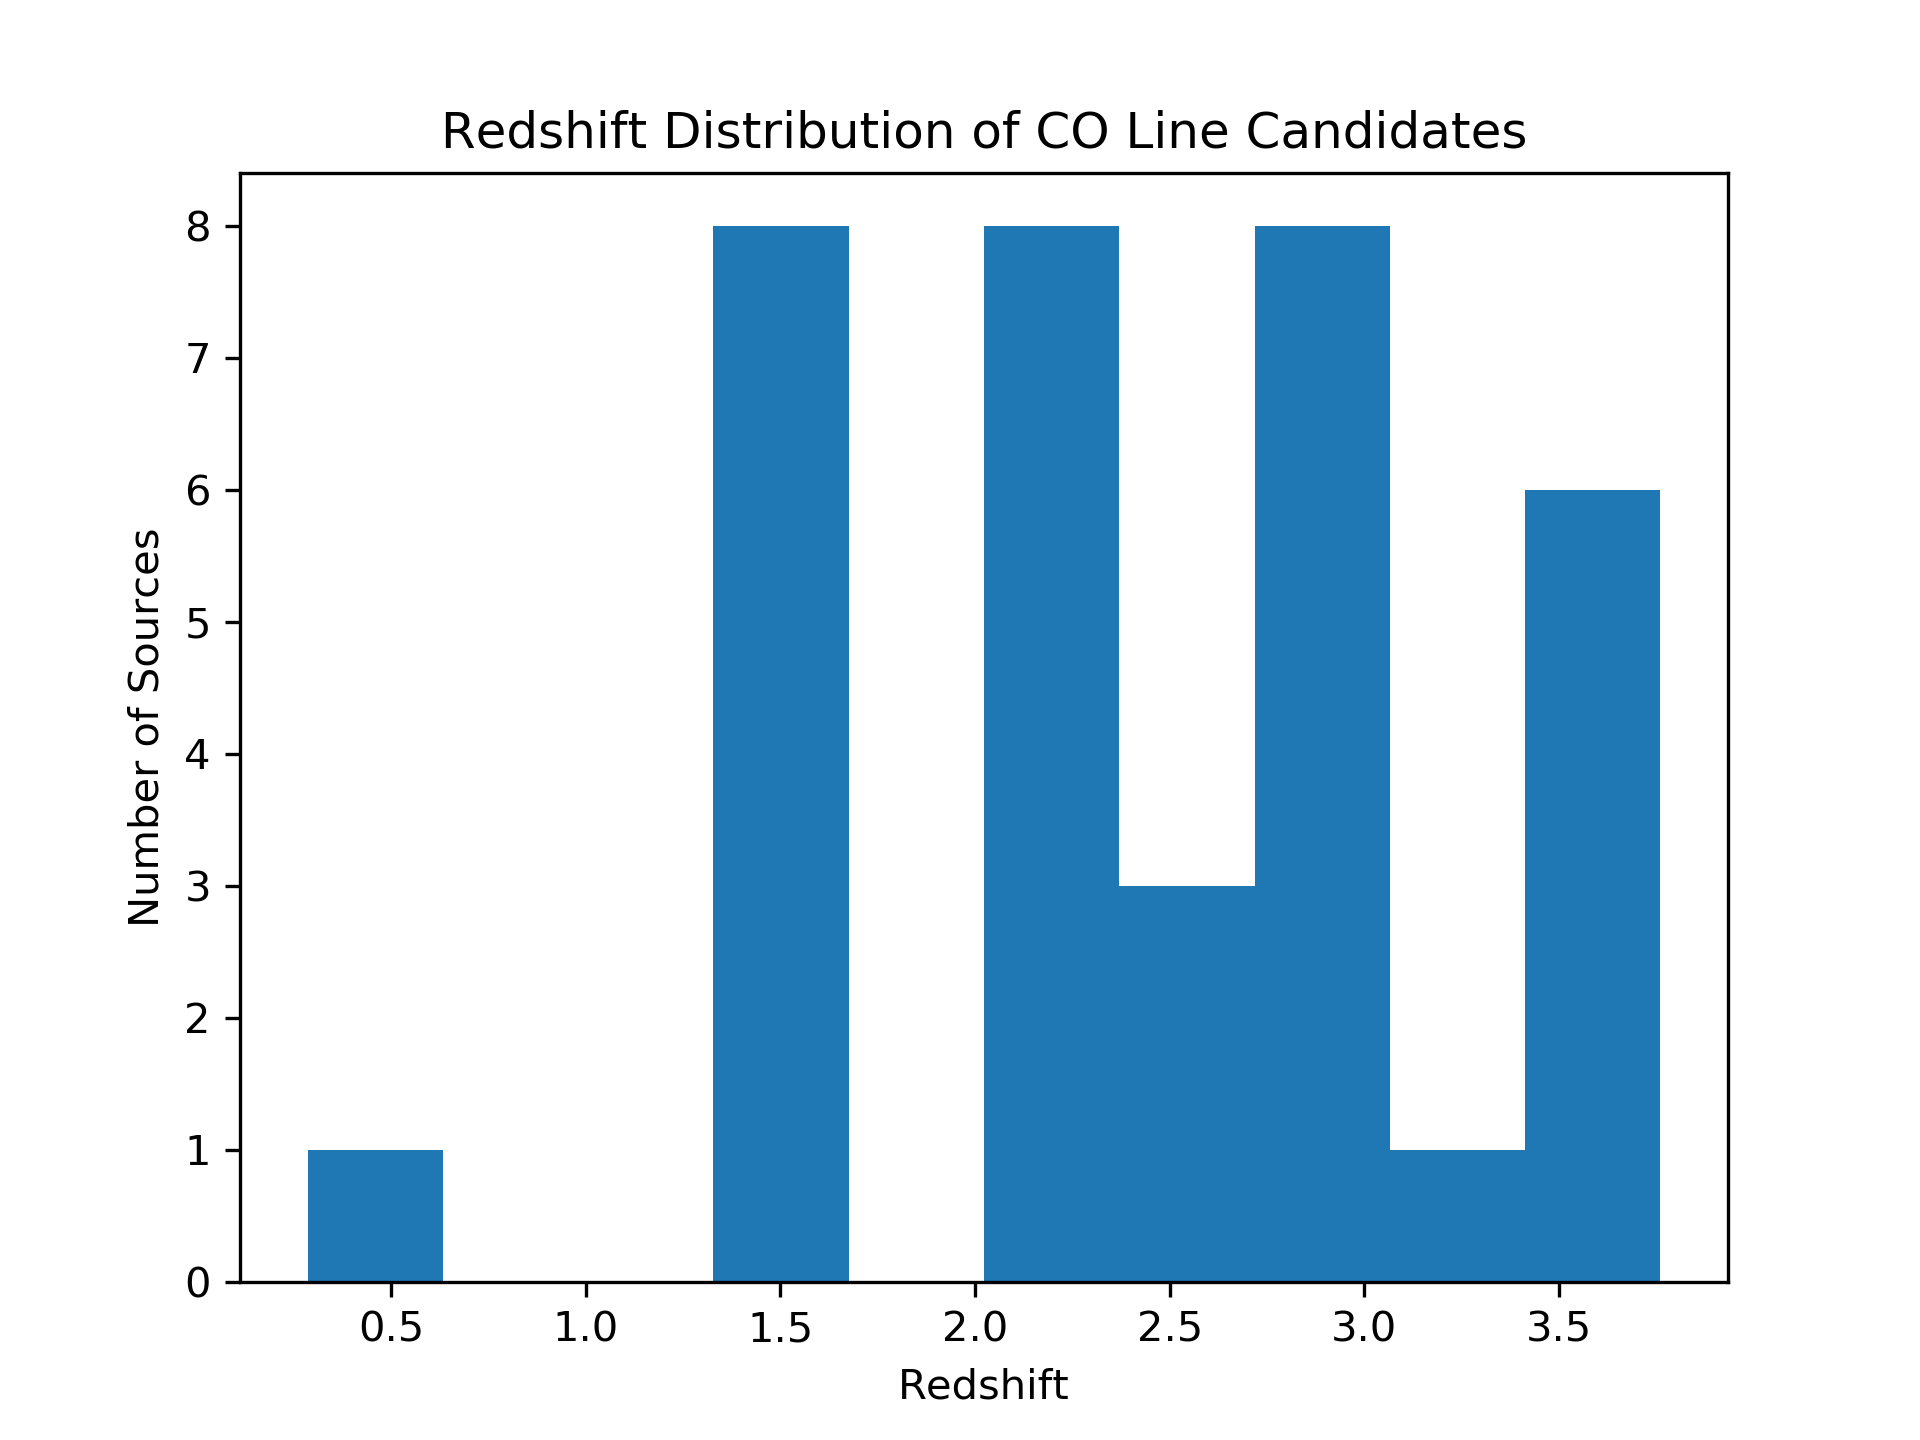
\includegraphics[width=120mm]{Survey/redshift_catalog.png}
\caption{Redshift distribution for all CO line candidate redshifts with a fidelity above 0.6, shown in Table \ref{table:Catalog}. These are the redshifts of the CO lines as determined by matching them to a CO transition, not including the redshifts of the 3 matched galaxies.}
\label{fig:cat_red}
\end{figure}

\section{Discussion}

Of the 35 line candidates chosen for the final catalog, only $\sim$9\% percent of the lines match to galaxies. Of those that do, only two matched to the most massive, most star-forming galaxies in the field. 

Possible explanations include issues with MAGPHYS' fitting of the galaxies in the catalog, as many of the galaxies seem poorly constrained. The errors in imprecise photometric redshifts could affect the estimation of the physical parameters, potentially explaining why one of the counterparts was not at the more massive end of the mass versus star-formation rate plot. The only counterpart with a spectroscopic redshift, ID.1's match, is also the counterpart with the highest stellar mass and star-formation rate, and the type of counterpart that was expected to be found in this survey.

Using a lower fidelity cut, such as a cut of $>$ 0.4, does not change the counterparts being unexpectedly composed primarily of lower stellar mass and star-forming galaxies, as seen in Fig. \ref{fig:fid_40_cross}. In fact, essentially all the extra matches from using a lower fidelity cut come from the galaxies that are the least massive and least star-forming in the field, suggesting that those matches might be spurious.

\begin{figure}[!htbp]
\centering 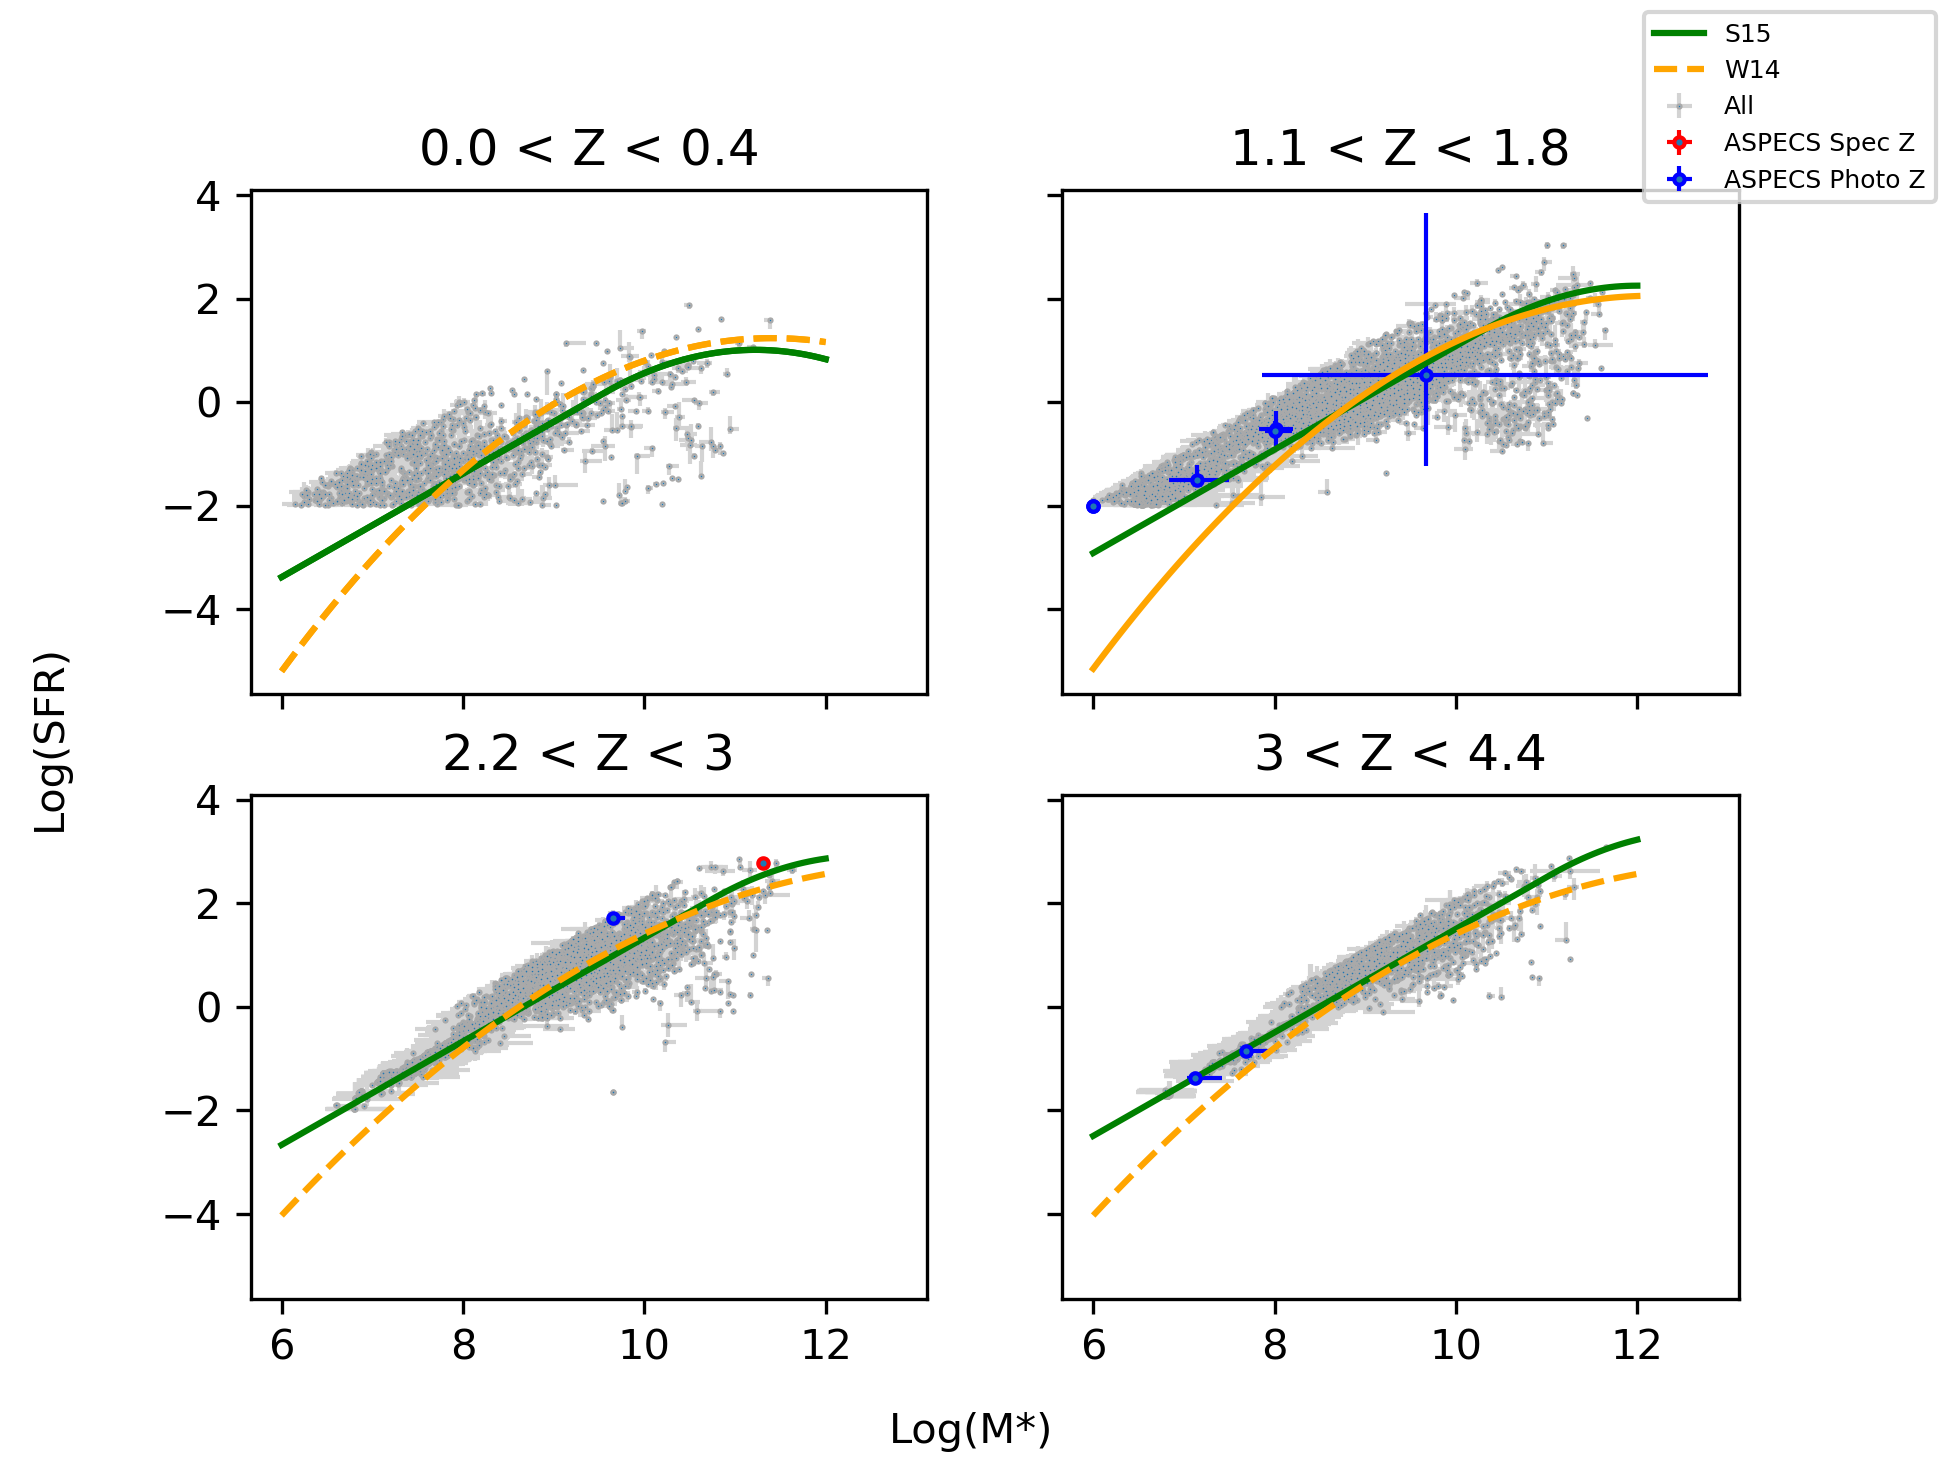
\includegraphics[width=120mm]{No_Cut_Mstar_vs_SFR_all_closest_sep_1_0_sn_fid_40.png}
\caption{Stellar mass versus star-formation rate for galaxies that the fidelity $>$ 0.4 CO line sample matched to. Red points are matched galaxies with spectroscopic redshifts, while blue points are matched galaxies with photometric redshifts. Grey points are all the galaxies in the compiled catalog from \ref{sec:ancillary}. The green lines are the galaxy main sequence fits from \cite{schreiber2015herschel}. The yellow line is from \cite{Whitaker_2014}'s galactic main sequence fit, where the solid line means it is computed within the range mentioned in the paper, while dotted means that the values are extrapolated from the paper to higher, or lower, redshifts. Two of the three matches are on the upper edge of the main sequence, the same two counterparts as for the fidelity $>$ 0.6 catalog, while the other matches have much lower stellar masses and star-formation rates than expected for this survey. Error bars are the 16/84th percentile outputs from MAGPHYS.}
\label{fig:fid_40_cross}
\end{figure}

% Physics based explanations

Other possible explanations include that the CO emitting galaxies are very dusty and optically dark, and so have not shown up in shorter wavelengths. Previous ASPECS surveys have found CO candidates without any obvious match to a previously known galaxy, along with the PdBI survey and COLDz \cite{decarli2014molecular, pavesi2018co}. This could mean that these CO lines without matches are too obscured in other wavelengths to have been detected before. As can be seen in \ref{sec:A1}, a significant number of the CO line candidates that do not match to a counterpart seem to exist in areas of the sky with very little or no other objects visible around them in optical wavelengths. 

%Try to expand a bit more this, you can also make some comments about the plot for the section fidelity cut that I suggested.

%It will maybe show more galaxies, but at lower stellar mass. You could mention that imprecise photometric errors could also affect the estimation of physical parameters (to mention a possible reason to explain why these are not at the more massive end as was expected. If you show me the plot with that cut, maybe I could give you more thoughts about what else to say.

\chapter{Clustering}

Wide ASPECS' well-defined, large cosmic volume allows for some of the first direct constraints on the clustering bias of CO emitters. This clustering bias can be then used to constrain the typical halo mass in which they reside. 

\section{Previous Work}

Previous work on clustering has been looked at different subpopulations of galaxies. Hickox et al. 2011 looked at the clustering of quasars and concealed quasars. Hickox et al. 2012 looks at the clustering in SMGs and compares them to clustering found in other surveys. 


[INCLUDE THE HICKOX et al. 2012 PLOT]
C

[1. show the 4 panel plot (for only 1 binding choice), with the different S/N cuts (or better for fidelity cuts, if that is not so time consuming to do), to show how the clustering signal is going up. 
2. Then explain how you selected your final sample (then selecting all candidates with fidelity >0.6) and show the clustering plot for that particular case. For this case show your preferred binning (and remember to choose the starting point of the first bin to have the minimum distances you measured between your candidates). 
3. Provide the final A and r0 parameters, and mention that you tested the sensitivity of the results with the binning choice (then maybe you can show your different binning choices for this same sample, and the r0 for each one)
4. we need to make some comments about this result (compare with others r0 in the literature, we can talk more about this). Make clear the point that the measurement is noisy and other strategies need to be done in the future.]

[I don’t think you need to provide details in your report about how the cross-correlation works but just mention that this technique would improve the statistics and just provide some reference of papers in which this technique is used for example Croom+04, Coil+07, Padmanabhan+09, Hickox+11, Hickox+12, etc.]

[Spatial correlation measure-
ments provide information about the characteristic bias and hence
mass of the haloes in which galaxies reside (e.g., Kaiser 1984;
Bardeen et al. 1986), and so provide a robust mass estimate that is
free of many of the systematics in measuring stellar or black hole
masses. The observed clustering of SMGs and QSOs can thus allow
us to test whether these populations are found in similar haloes and
so may evolve into each other over short timescales. \cite{hickox2011clustering} 2012]

\begin{figure}[tbp]
\centering 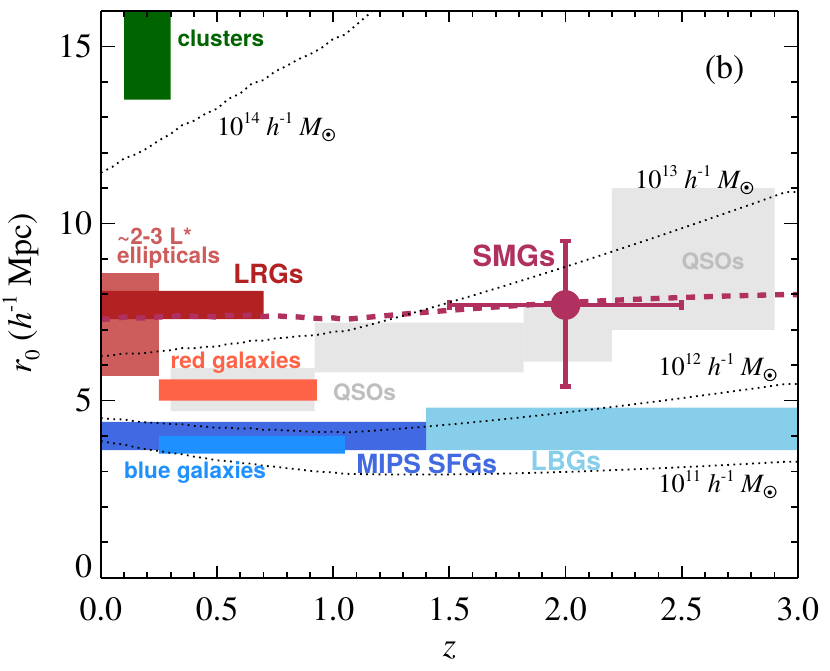
\includegraphics[width=120mm]{clustering/Hickox2012_Compare.png}
\caption{$r_0$ values for a variety of celestial objects as a function of redshift. Figure adapted from \cite{10.1111/j.1365-2966.2011.20303.x}.}
\label{fig:Hickox_compare}
\end{figure}

\section{Method}

\subsection{Autocorrelation Function}

The clustering is computed through a two point correlation function. The first step s to calculate the angular correlation function $ \omega(\theta)$. Once $ \omega(\theta)$ is computed, the second step is to obtain the two-point correlation function parameters of $r_0$ and $\gamma$.

The two-point correlation function is the the probability above Poisson of finding a galaxy in a volume element $dV$ at a physical separation $r$ from another randomly chosen galaxy, such that $$ dP = n[1 + \Eta(r)]dV$$, [REWORD] where $n$ is the mean space density of the galaxies in the sample. The estimator comes from Landy \& Szalay (1993) where $$ \omega(\theta) = \frac{1}{RR}(DD-2DR + RR)$$, there $DD$, $DR$, and $RR$ are the number of data-data, data-random, and random-random galaxy pairs at a separation $\theta$, where each of the three collections is normalized to sum to 1. 

Once the angular correlation function is found, a power-law model is fitted following $$\omega(\theta) = A\theta^{-\beta} $$

In this report, $\beta$ = 0.8, a value found for many other galaxy autocorrelations [CITE]. To convert the $A$ and $\beta$ to real-space $r_0$ and $\gamma$, the conversion can be found through the two equations

$$ \gamma = \beta + 1 $$ $$ A = H_{\gamma}\frac{\int_{0}^{\inf} (dN_1/dz)(dN_2/dz)E_z\chi^{1 - \gamma} dz}{[\int_{0}^{\inf} (dN_1/dz)dz][\int_{0}^{\inf} (dN_2/dz)dz]}r_0^{\gamma}$$

where $H_{\gamma} = \Gamma(0.5)\Gamma(0.5[\gamma -1])\Gamma(0.5\gamma)$, where $\Gamma$ is the gamma function, $\chi$ is the radial comoving distance, $dN_{1,2}/dz$ are the redshift distributions of the samples, where in the case of autocorrelation, are equal to each other, and $E_z = H_z/c = dz/d\chi$ \cite{hickox2011clustering}. The Hubble parameter $H_z$ can be found from
$$H_z^2 = H_0^2[\Omega_m(1+z)^3 + \Omega_{\lambda}]$$ \cite{hickox2011clustering}.

For this analysis, all CO line candidates above the 0.6 fidelity threshold were used, resulting in 35 sources, shown in Fig. \ref{fig:Clustering_points}. Two catalogs of random points were created and their angular correlation computed to show that it is consistent with zero, shown in Fig.\ref{fig:random_points}. As a comparison, the two point correlation function was also computed for other fidelity cuts. The redshift distribution was taken from the CO redshifts of the lines, and the calculations were calculated over the range z = 1.5 to 3.5, as this is where the majority of the CO lines' redshifts are. Results over the range of z = 0 to z = 4.4 are also shown. 

\begin{figure}[tbp]
\centering 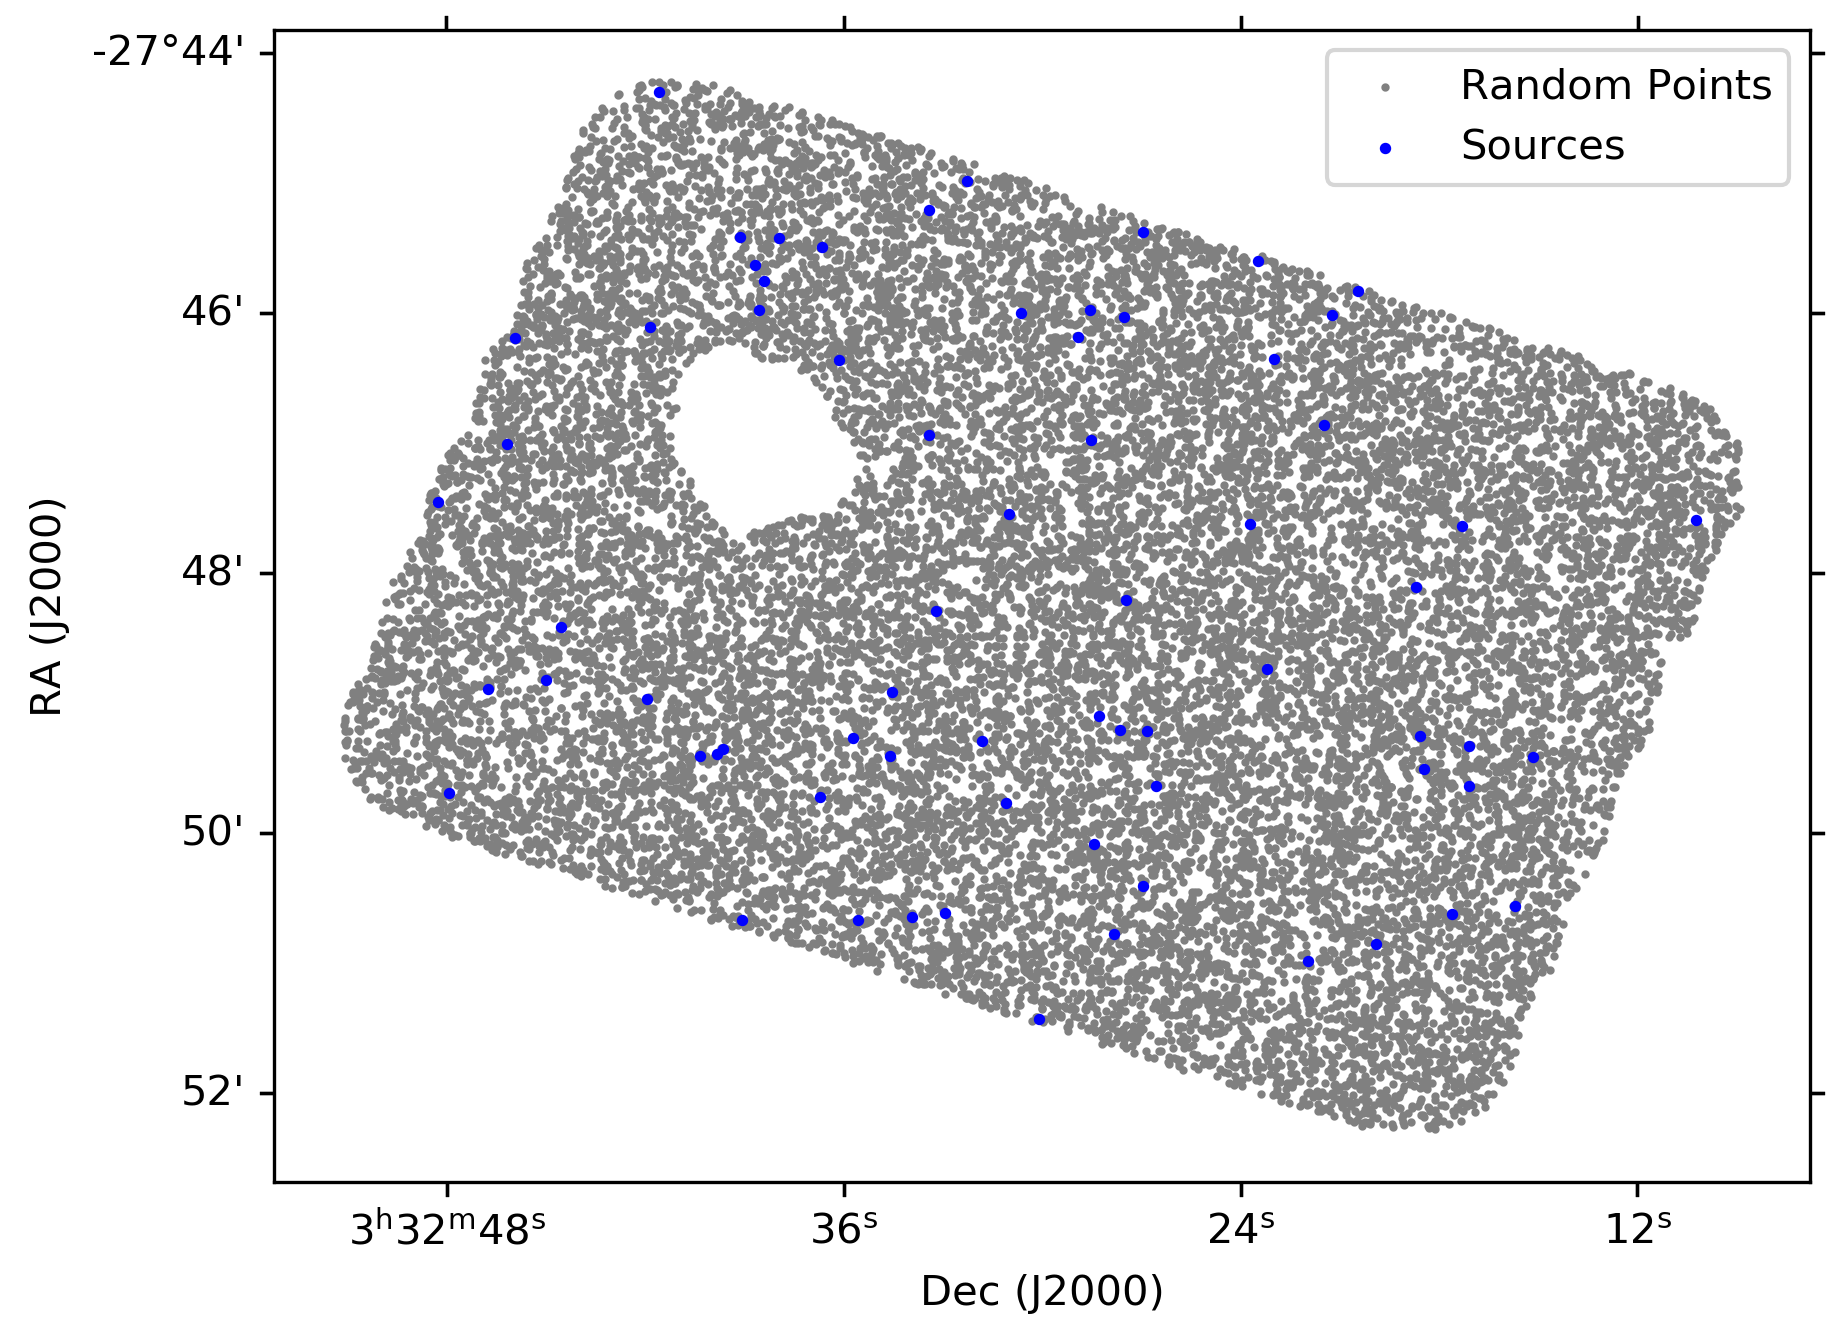
\includegraphics[width=120mm]{PDFS/NX_V_Y_Sources_20000.png}
\caption{Random points and sources from the $>$ 0.6 fidelity cut. The random points are distributed uniformly throughout the Wide ASPECS footprint.}
\label{fig:Clustering_points}
\end{figure}

\begin{figure}[tbp]
\centering 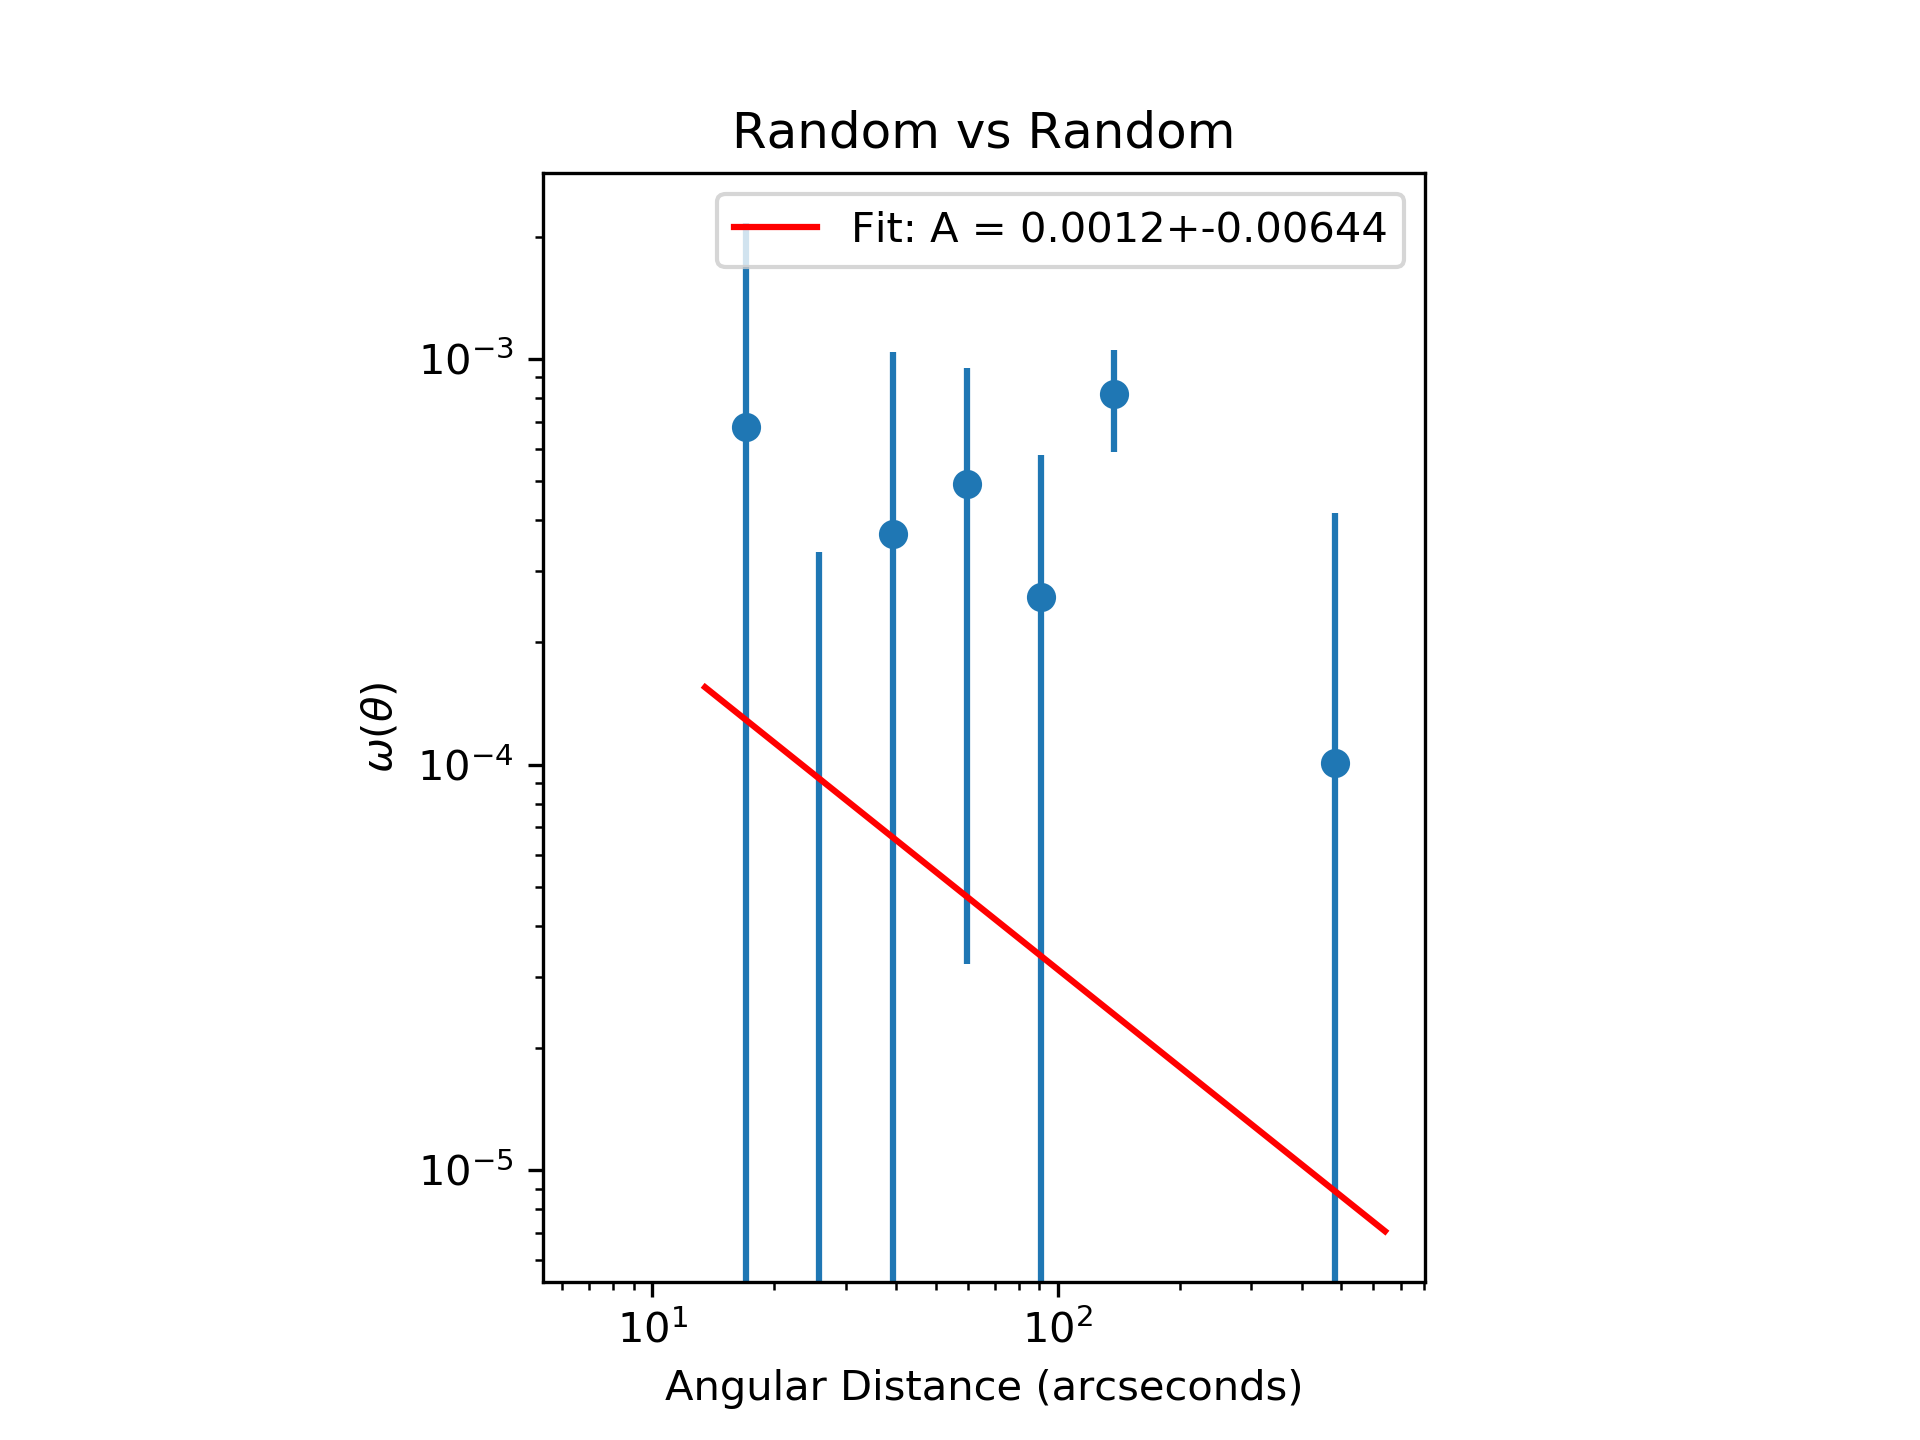
\includegraphics[width=120mm]{clustering/Log_Random_vs_Random_15000NoParenFlip_bin10.png}
\caption{Angular correlation two sets of random points used in this analysis, showing that the angular correlation is consistent with zero, as would be expected for uniformly distributed points.}
\label{fig:random_points}
\end{figure}

\subsection{Projected Correlation Function}

[INCLUDE PROJECTED ONE? SINCE NEED IT FOR THE DM CALCULATION?]

\subsection{Halo Mass Calculation}

To determine the halo mass from the calculations[INCLUDE HALO MASS CALCULATIONS]

\cite{hickox2011clustering} used the HALOFIT code of Smith et al. 2003, to determine the non-linear power spectrum $\Delta_{NL}^2(k,z)$ of dark matter, assuming the cosmology and the slope of the initial fluctuation power spectrum $\Gamma = \Omega_mh = 0.21$. The Fourier transform of the nonlinear-dimensionless power spectrum gives the real-sapce correlation function $\Eta(r)$, which is then integrated to $\pi = 100 h^{-1} Mpc$ following Equation [INSERT] to obtain the dar kmatter projected correlation function $\omega^{DM}_p(R,z)$.

To obtain $\omega(\theta)$ for the dark matter, Limber's equation is used to project the power spectrum into the angular correlation. Specifically a Monte Carlo integration of Equation (A6) in Myers et al. 2007 is used to obtain $\omega(\theta)$ for dark matter. For each angular correlation analysis, we compute the average ration between the best-fit power law model and the dark matter $\omega(\theta)$ on scales from 8 arcminutes to 50 arcminutes, where $\omega(\theta$ is dominated by the two-halo term. This ratio gives us $b^2_{CO}$ for the CO autocorrelations. 

Finally, using $b^2_{CO}$ to estimate the charactersitic mass of the dark matter halos hosting each subset of galaxies. Sheth et al. 2001 derived a relation betwwen dark-matter halo mass and large-scale bias that agrees well with the results of comsological simulations. We use Eqn. (8) of Sheth et al. 2001 to convert $b_{C)}$ and $M_{halo}$, we obtain esimtaes for $M_{halo}$. 

\section{Results}

As can be seen in Fig. \ref{fig:Angular_correlation}, as the fidelity increases, $A$ increases as well. The change is most significant when only fitting the positive points.  When converted to $r_0$, the fidelity cuts result in $r_0$ values of 23 +- 5 for fidelity $>$ 0.7, 20 +- 2 for fidelity $>$ 0.6, 8 +- 1.5 for fidelity $>$ 0.5, and no $r_0$ for fidelity > 0.4, as the $A$ value is consistent with 0. 

\begin{figure}[tbp]
\centering 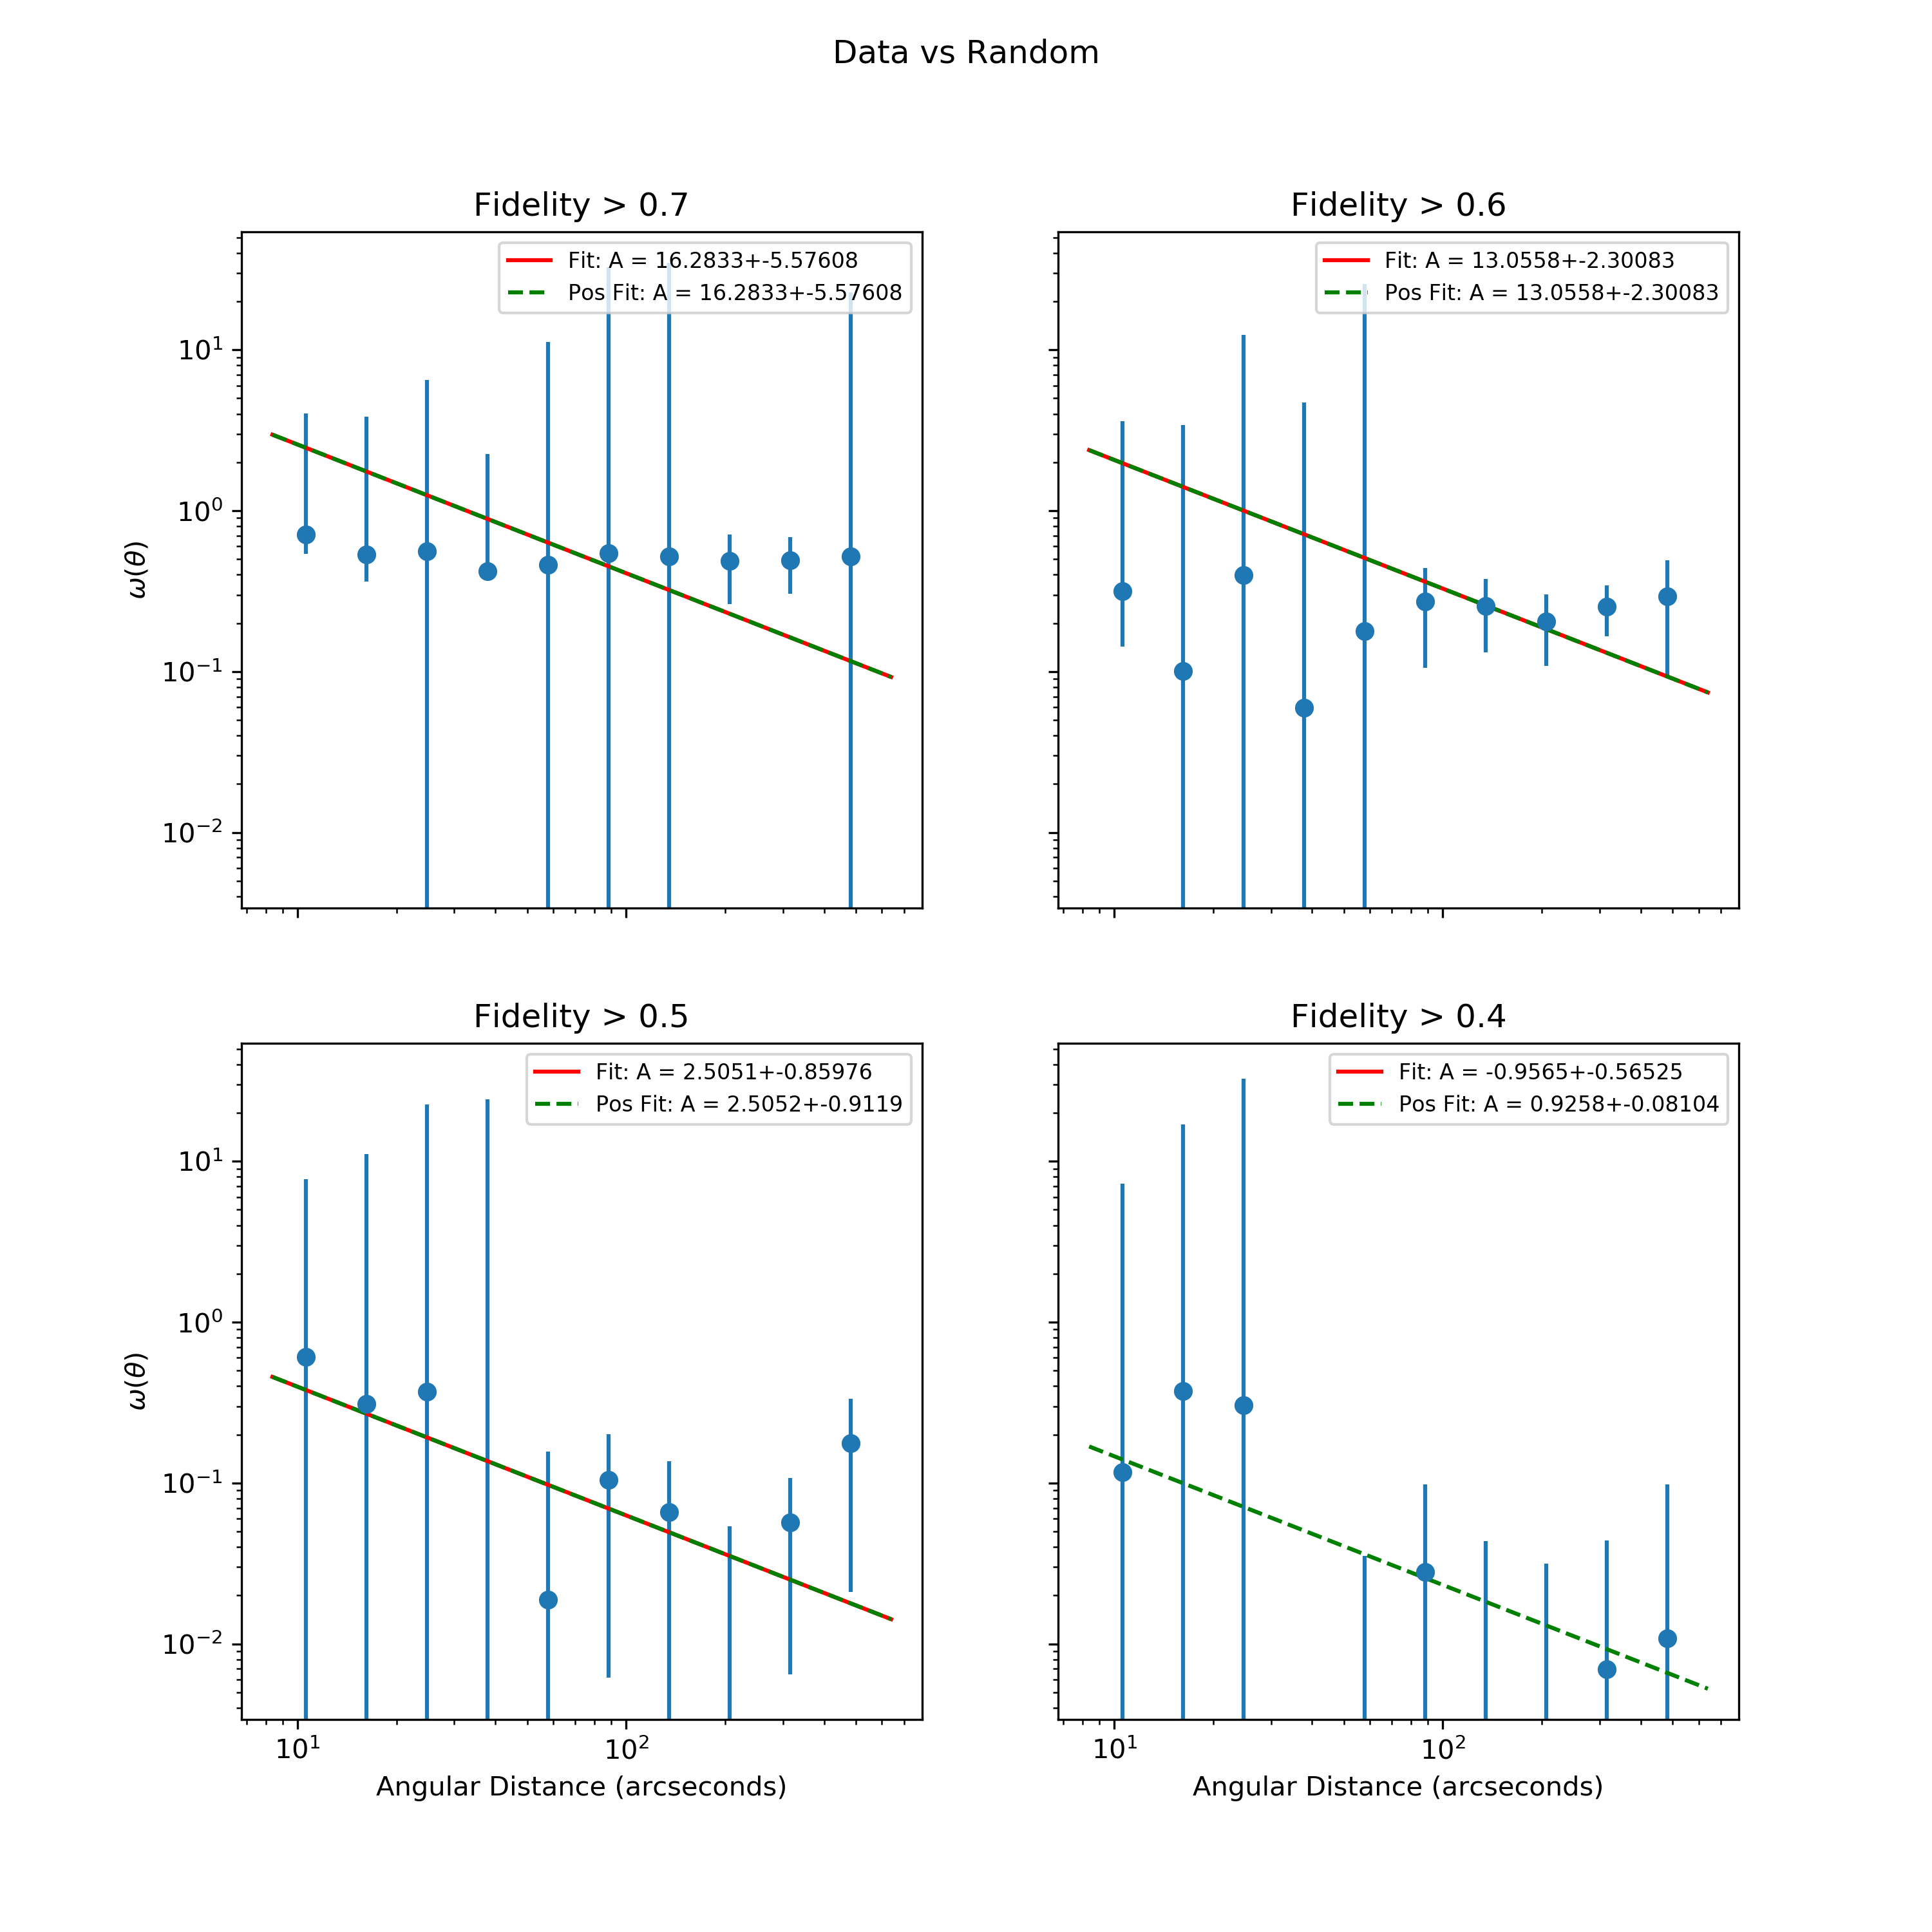
\includegraphics[width=120mm]{Fidelity/Log_4Panel_Data_Vs_Random_bin10_NFalse_Num10000.png}
\caption{Angular correlation function for various fidelity cuts. The red lines are from fitting $\omega(\theta) = A\theta^{-0.8} $ to all of the bins. The green dashed line is from fitting that same equation only to bins that had a positive value. As the fidelity goes up, the $A$ value increases as well, indicating stronger clustering, as is expected.}
\label{fig:Angular_correlation}
\end{figure}

Besides the different fidelity cuts, different binnings also are included to study their effects on the final $r_0$ results. The results seem to be very dependent on the binning. While the values for the only positively fitted bins does not change dramatically as the binning changes, the number of bins does make a different whether there are enough 

\begin{figure}[tbp]
\centering 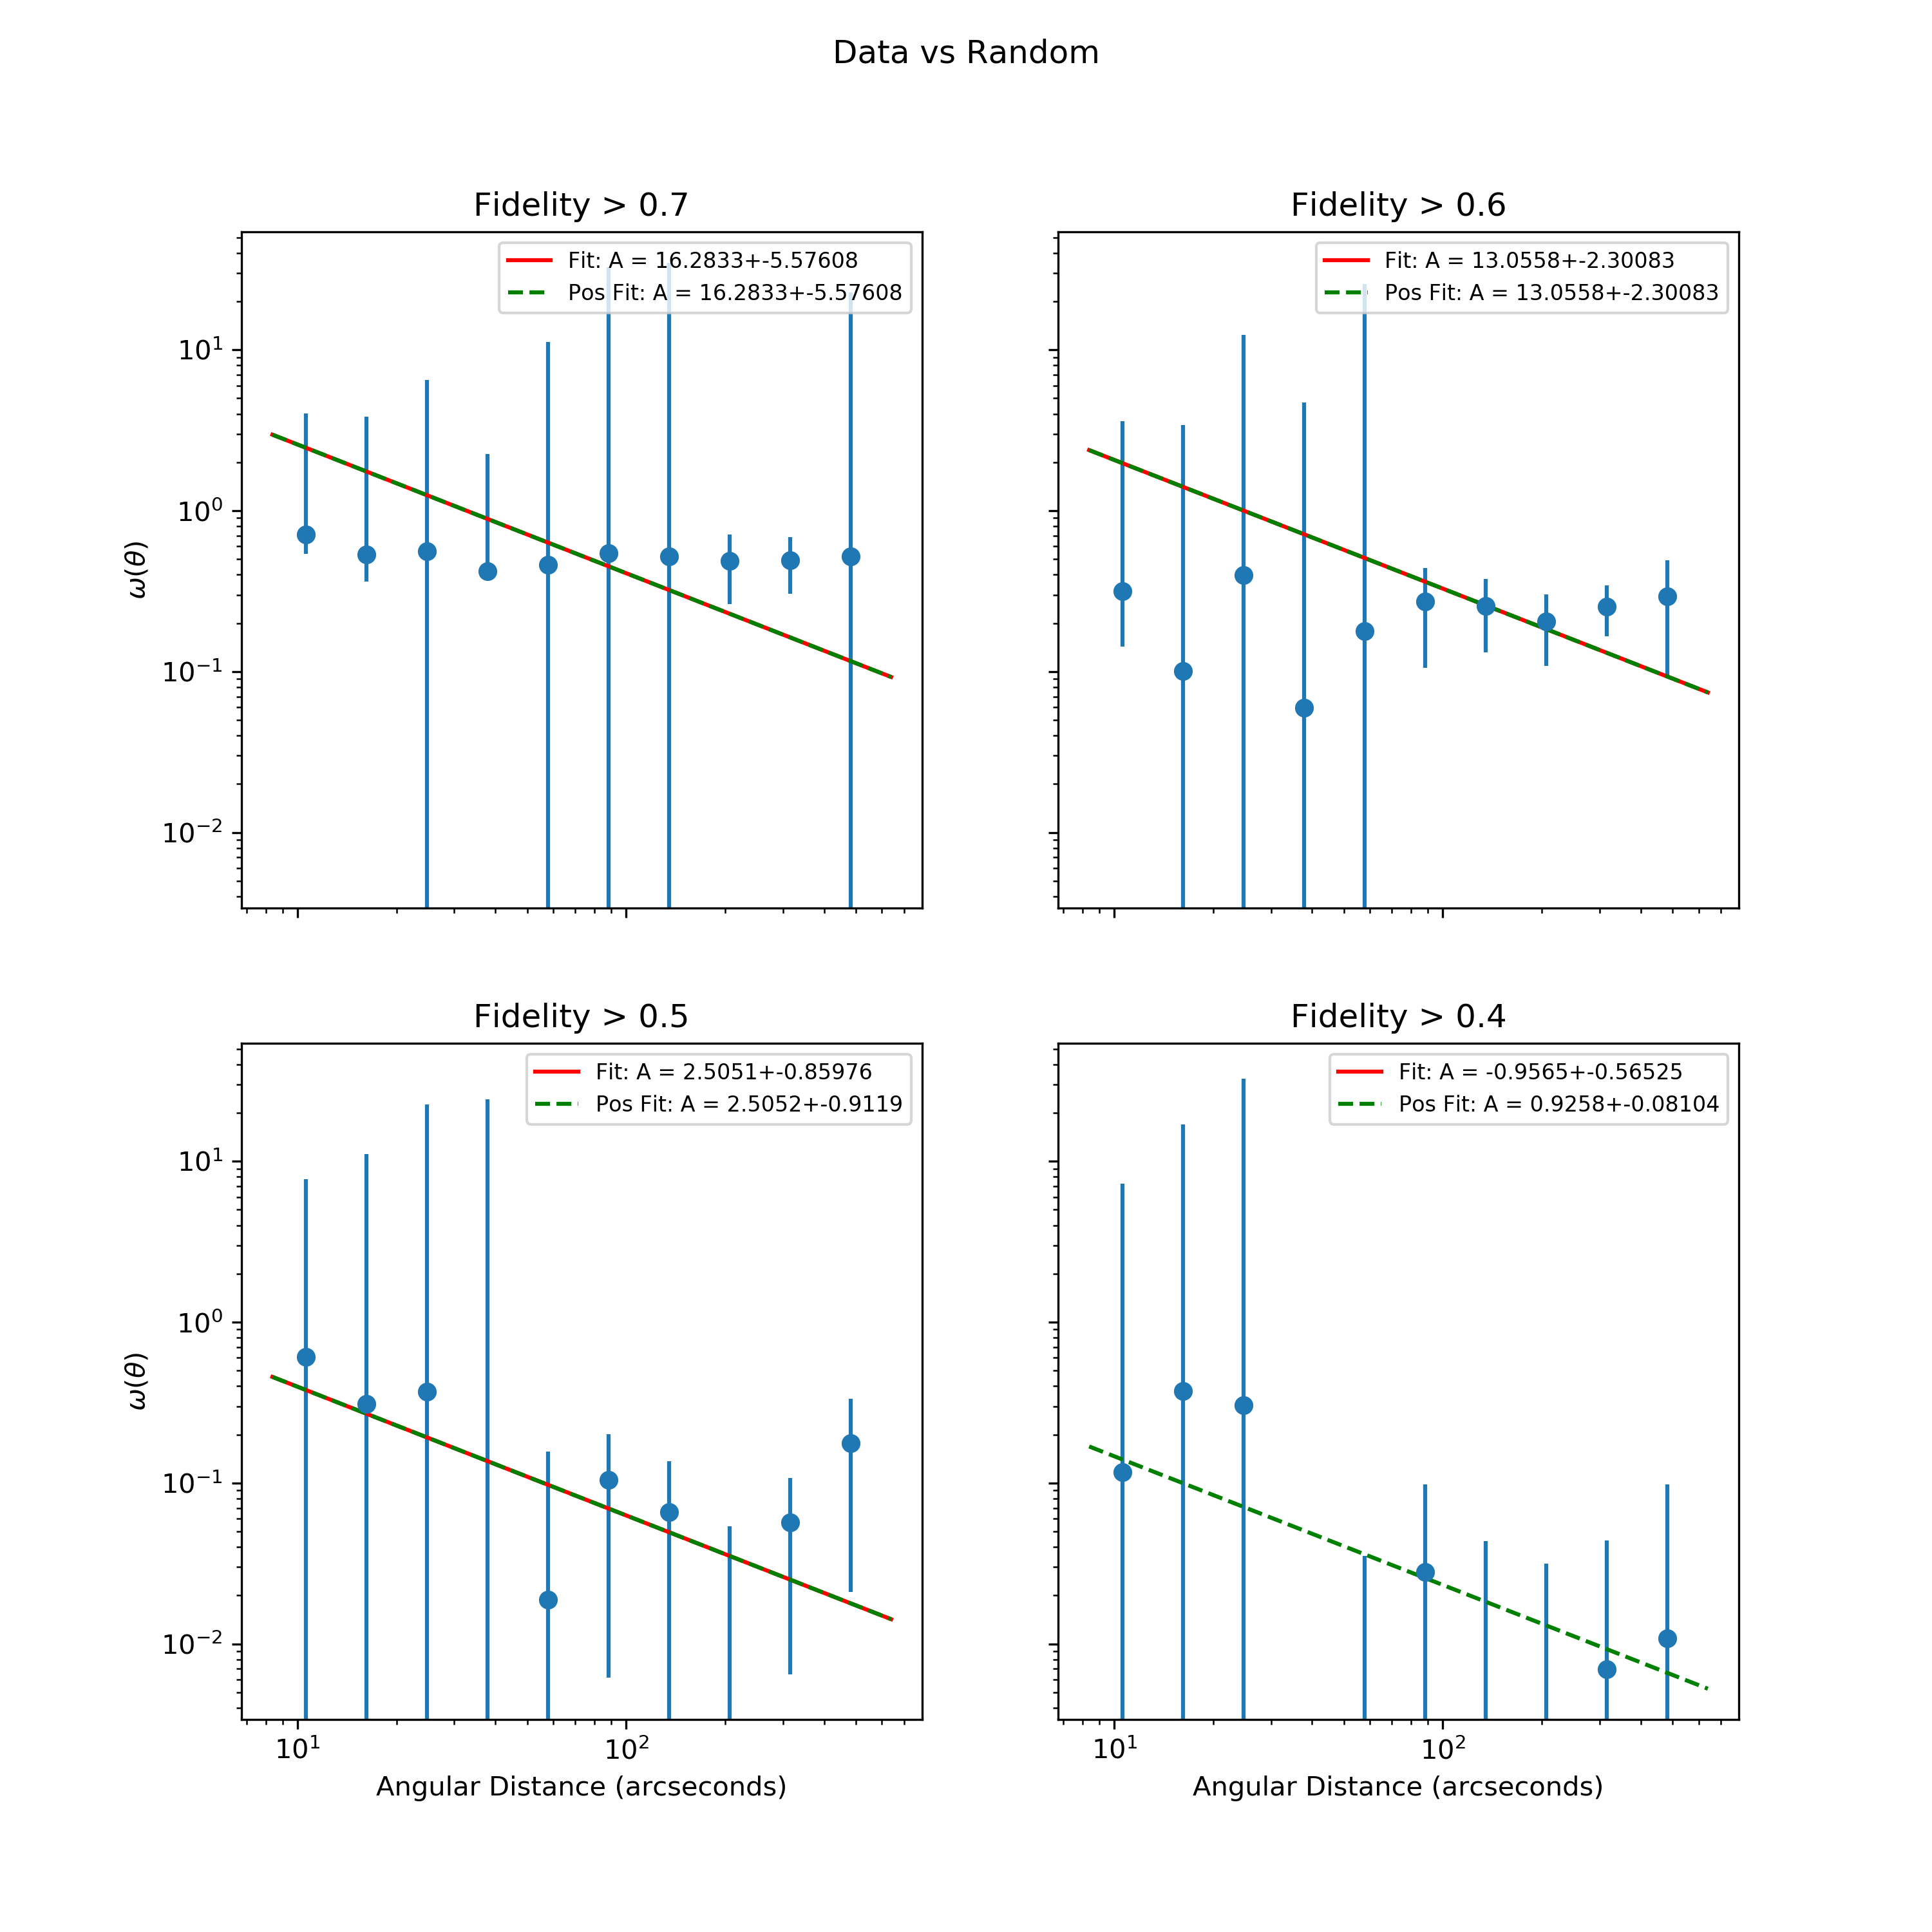
\includegraphics[width=120mm]{Fidelity/Log_4Panel_Data_Vs_Random_bin10_NFalse_Num10000.png}
\caption{Angular correlation function for various binnings.}
\label{fig:Angular_binnings}
\end{figure}

As should be expected, as the fidelity cut goes up, meaning a larger portion of the CO lines remaining are true sources, the clustering value becomes larger as well. Once the fidelity drops below 0.5, such that the majority of the lines should be false positives, the clustering values drop to be consistent with 0. The clustering values for a variety of fidelity cuts are shown in Table \ref{table:Clsutering}

[INCLUDE CLUSTERING TABLE HERE WITH RESULTS, A, r0, errors on both, number of sources used in each] \label{table:Clustering}

[INCLUDE PLOT OF DIFFERENT R0 VALUES DEPENDENT ON CLUSTERING -> HOW THAT AFFECTS THE VALUES]

[INCLUDE REDSHIFT DISTRIBUTION PLOT]

[TALK ABOUT DIFFERENCES BETWEEN LINEAR AND GAUSSIAN SENSETIVITY]

\section{Discussion}

The clustering results do show that there is a larger $r_0$ as the fidelity cut becomes higher, suggesting that there are real sources in the sample. On the other hand, the clustering measurement is still very noisy and future work will be required to get a better final clustering measurement. 

In comparison to other clustering measurements, \cite{hickox2011clustering} found an $r_0$ for quasers to be between 5.5 and 

\cite{hickox2011clustering} showed that for SMG galaxies, around a redshift of 2, the autocorrelation length $r_0 \approx 6 h^{-1} Mpc$. 

[INCLUDE DISCUSSION OF CLUSTERING OF OTHER GALAXY TYPES, HOW ODDLY HIGH THIS IS]

[WHY THE HIGH FIDELITY ONES MIGHT BE SO CLUSTERED AND BRIGHT?]



\chapter{Conclusion}

In this research, data from Wide ASPECS was used to find CO line candidates, determine their properties, and find their clustering bias. 

A catalog of 35 line candidates was created. This catalog was cross-matched to a catalog of previous detected galaxies in the same area. A total of three counterparts were found, and their properties were compared to the population of galaxies in the catalog. Two of those counterparts are on, or slightly above, the main sequence, while one has a much smaller stellar mass and star formation rate than would be expected for this survey. The other 32 potential sources could be optically dark, gas-rich galaxies that have evaded detection until now. 

Additionally, using the 35 CO lines in the catalog, the scale radius $r_0$ was computed and compared to other populations of galaxies. The scale radius seems to be similar to the $r_0$ of SMGs

% People will ask you if you tried to repeat your experiment by adopting priors in your line candidate selection. E.g., if you require that lines have an IRAC counterpart or a MUSE counterpart, you significantly drop the number of independent elements (and thus, the noise), which results in a superior fidelity. However, the drawback is that you introduce a selection function that you will have to account for in your clustering analysis. I suggest to add a few lines on this.

\section{Future Work}

While these results are interesting, they are quite tentative. The clustering results could be improved through performing the cross-correlation between the CO line candidates and the galaxy catalog \cite{hickox2011clustering, 10.1111/j.1365-2966.2011.20303.x, 10.1111/j.1365-2966.2008.14071.x}. 

Additional work could be done to verify the CO lines matched to galaxies, and investigate the reasons as to why the matched galaxies are much less massive and star forming than expected.

Priors could also be adopted for the line candidate search. For example, requiring lines have an IRAC or MUSE counterpart would reduce the number of independent elements, and therefore the noise, resulting in a higher fidelity. A drawback is that then the search is not a blind search, and the selection function would have to be accounted for in the clustering analysis.

\appendix
\chapter{Appendix}

\section{Line Candidate Cutouts}\label{sec:A1}

The following plots show the 35 CO line candidates in various wavelengths. The red contours show the +2$\sigma$,4$\sigma$, and 6$\sigma$ values in the datacubes. All cutouts are 3x3 arcseconds in size.

\begin{figure}[tbp]
\centering 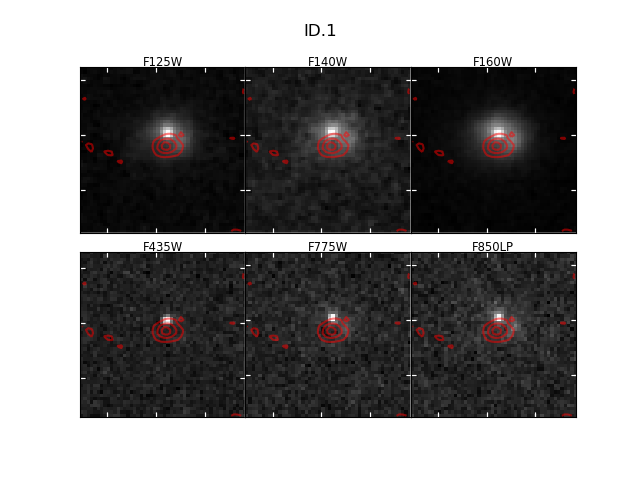
\includegraphics[width=160mm]{Matched/ASPECS_Cutout_0.png}
\caption{ID.1. Red contours signify +2$\sigma$,4$\sigma$, and 6$\sigma$. The size of the cutouts are 3x3 arcseconds. The spacing between the ticks is one arcsecond.}
\label{fig:Match_One}
\end{figure}

\begin{figure}[tbp]
\centering 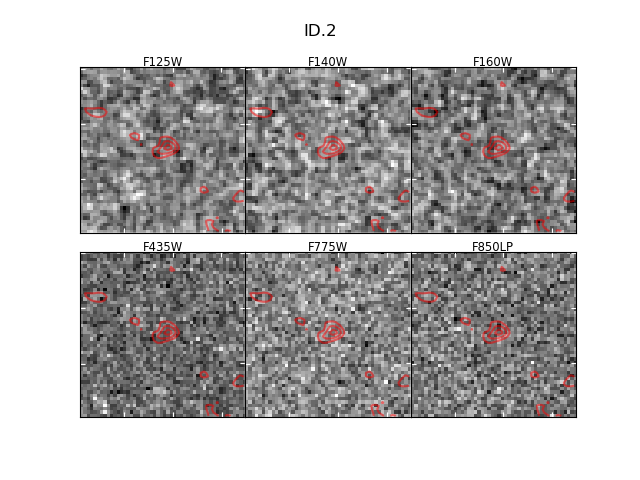
\includegraphics[width=160mm]{Matched/ASPECS_Cutout_1.png}
\caption{ID.2. Same contours and cutout size as for \ref{fig:Match_One}.}
\label{fig:Match_Two}
\end{figure}


\begin{figure}[tbp]
\centering 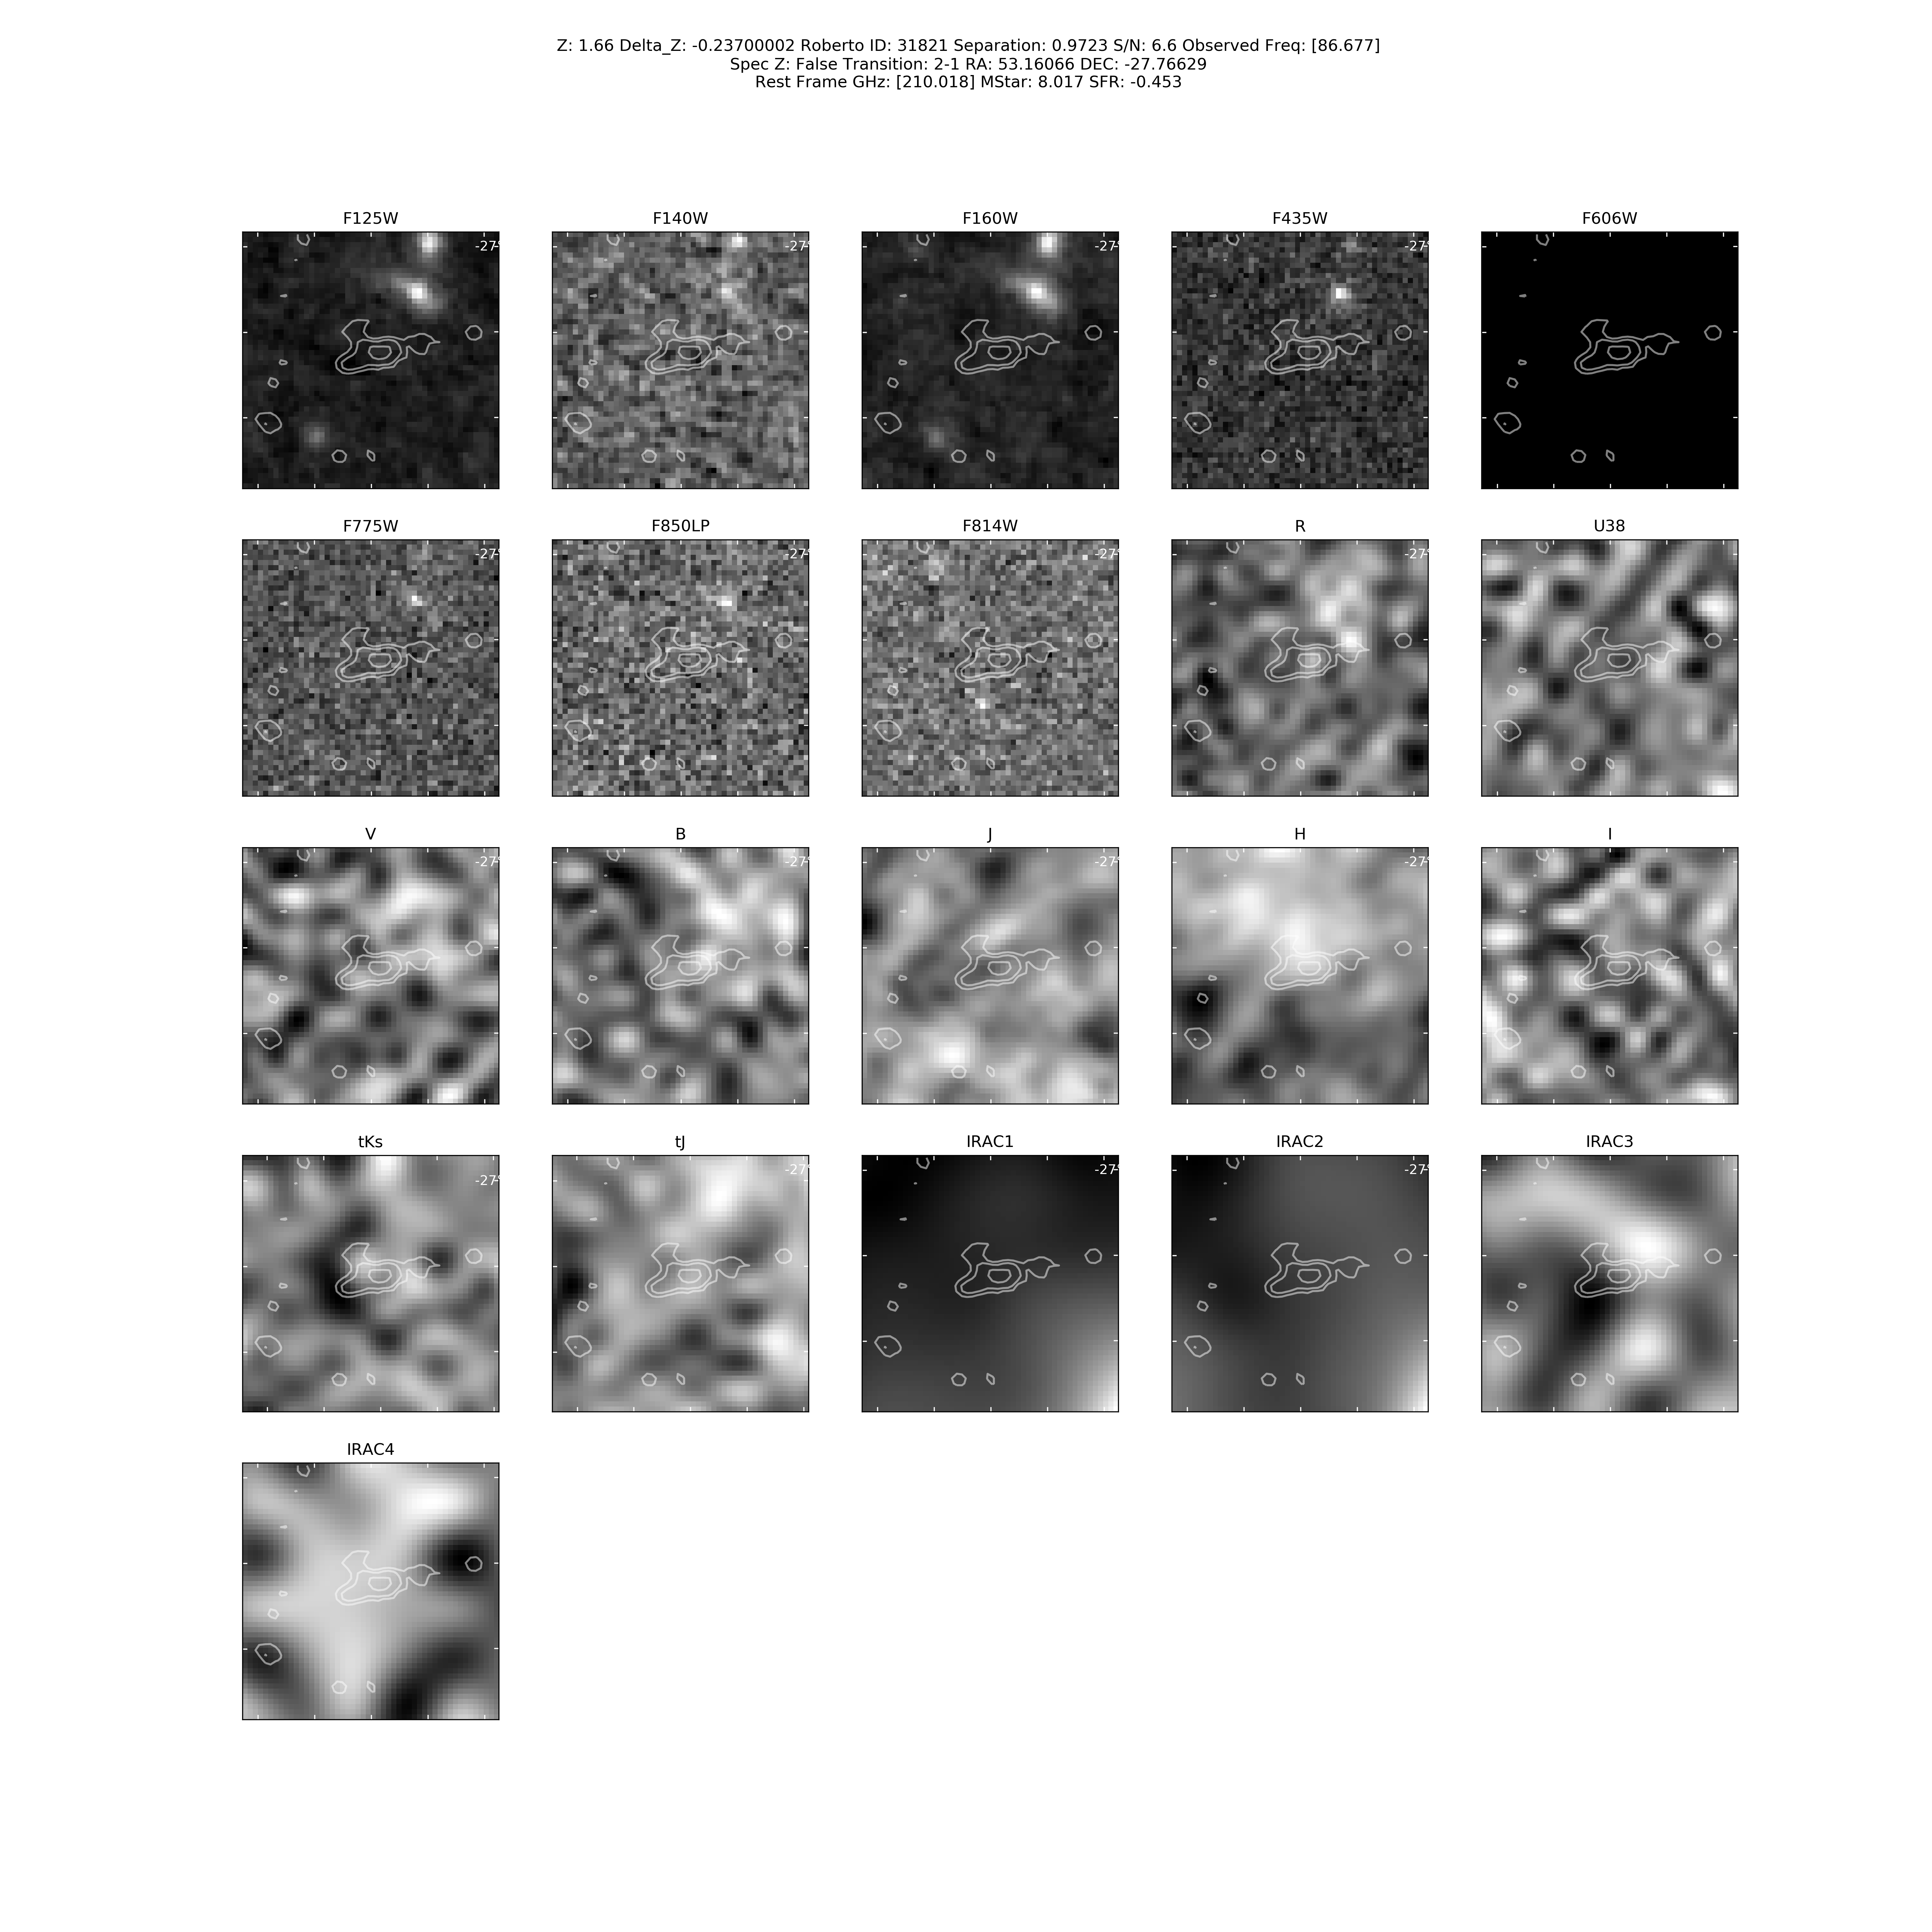
\includegraphics[width=160mm]{Matched/ASPECS_Cutout_2.png}
\caption{ID.3. Same contours and cutout size as for \ref{fig:Match_One}.}
\label{fig:Match_Three}
\end{figure}

\begin{figure}[tbp]
\centering 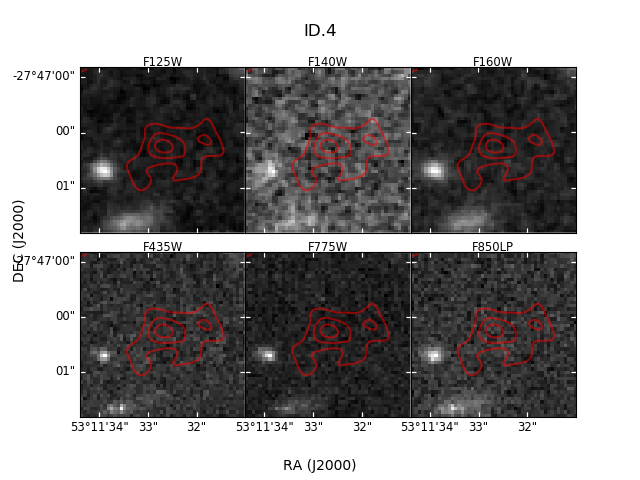
\includegraphics[width=160mm]{Matched/ASPECS_Cutout_3.png}
\caption{ID.4. Same contours and cutout size as for \ref{fig:Match_One}.}
\label{fig:Match_Three}
\end{figure}

\begin{figure}[tbp]
\centering 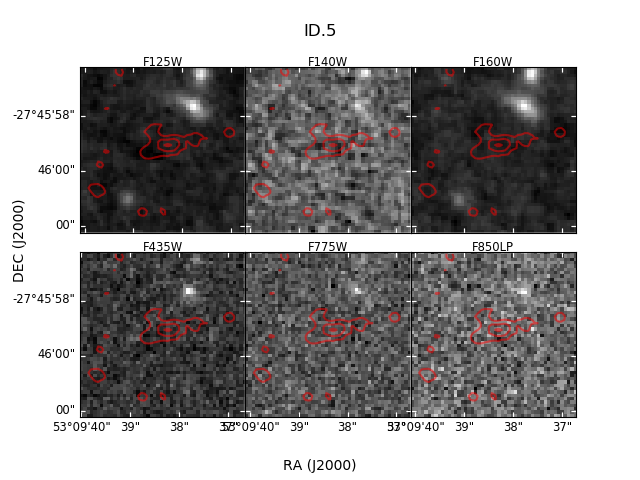
\includegraphics[width=160mm]{Matched/ASPECS_Cutout_4.png}
\caption{ID.5. Same contours and cutout size as for \ref{fig:Match_One}.}
\label{fig:Match_Four}
\end{figure}

\begin{figure}[tbp]
\centering 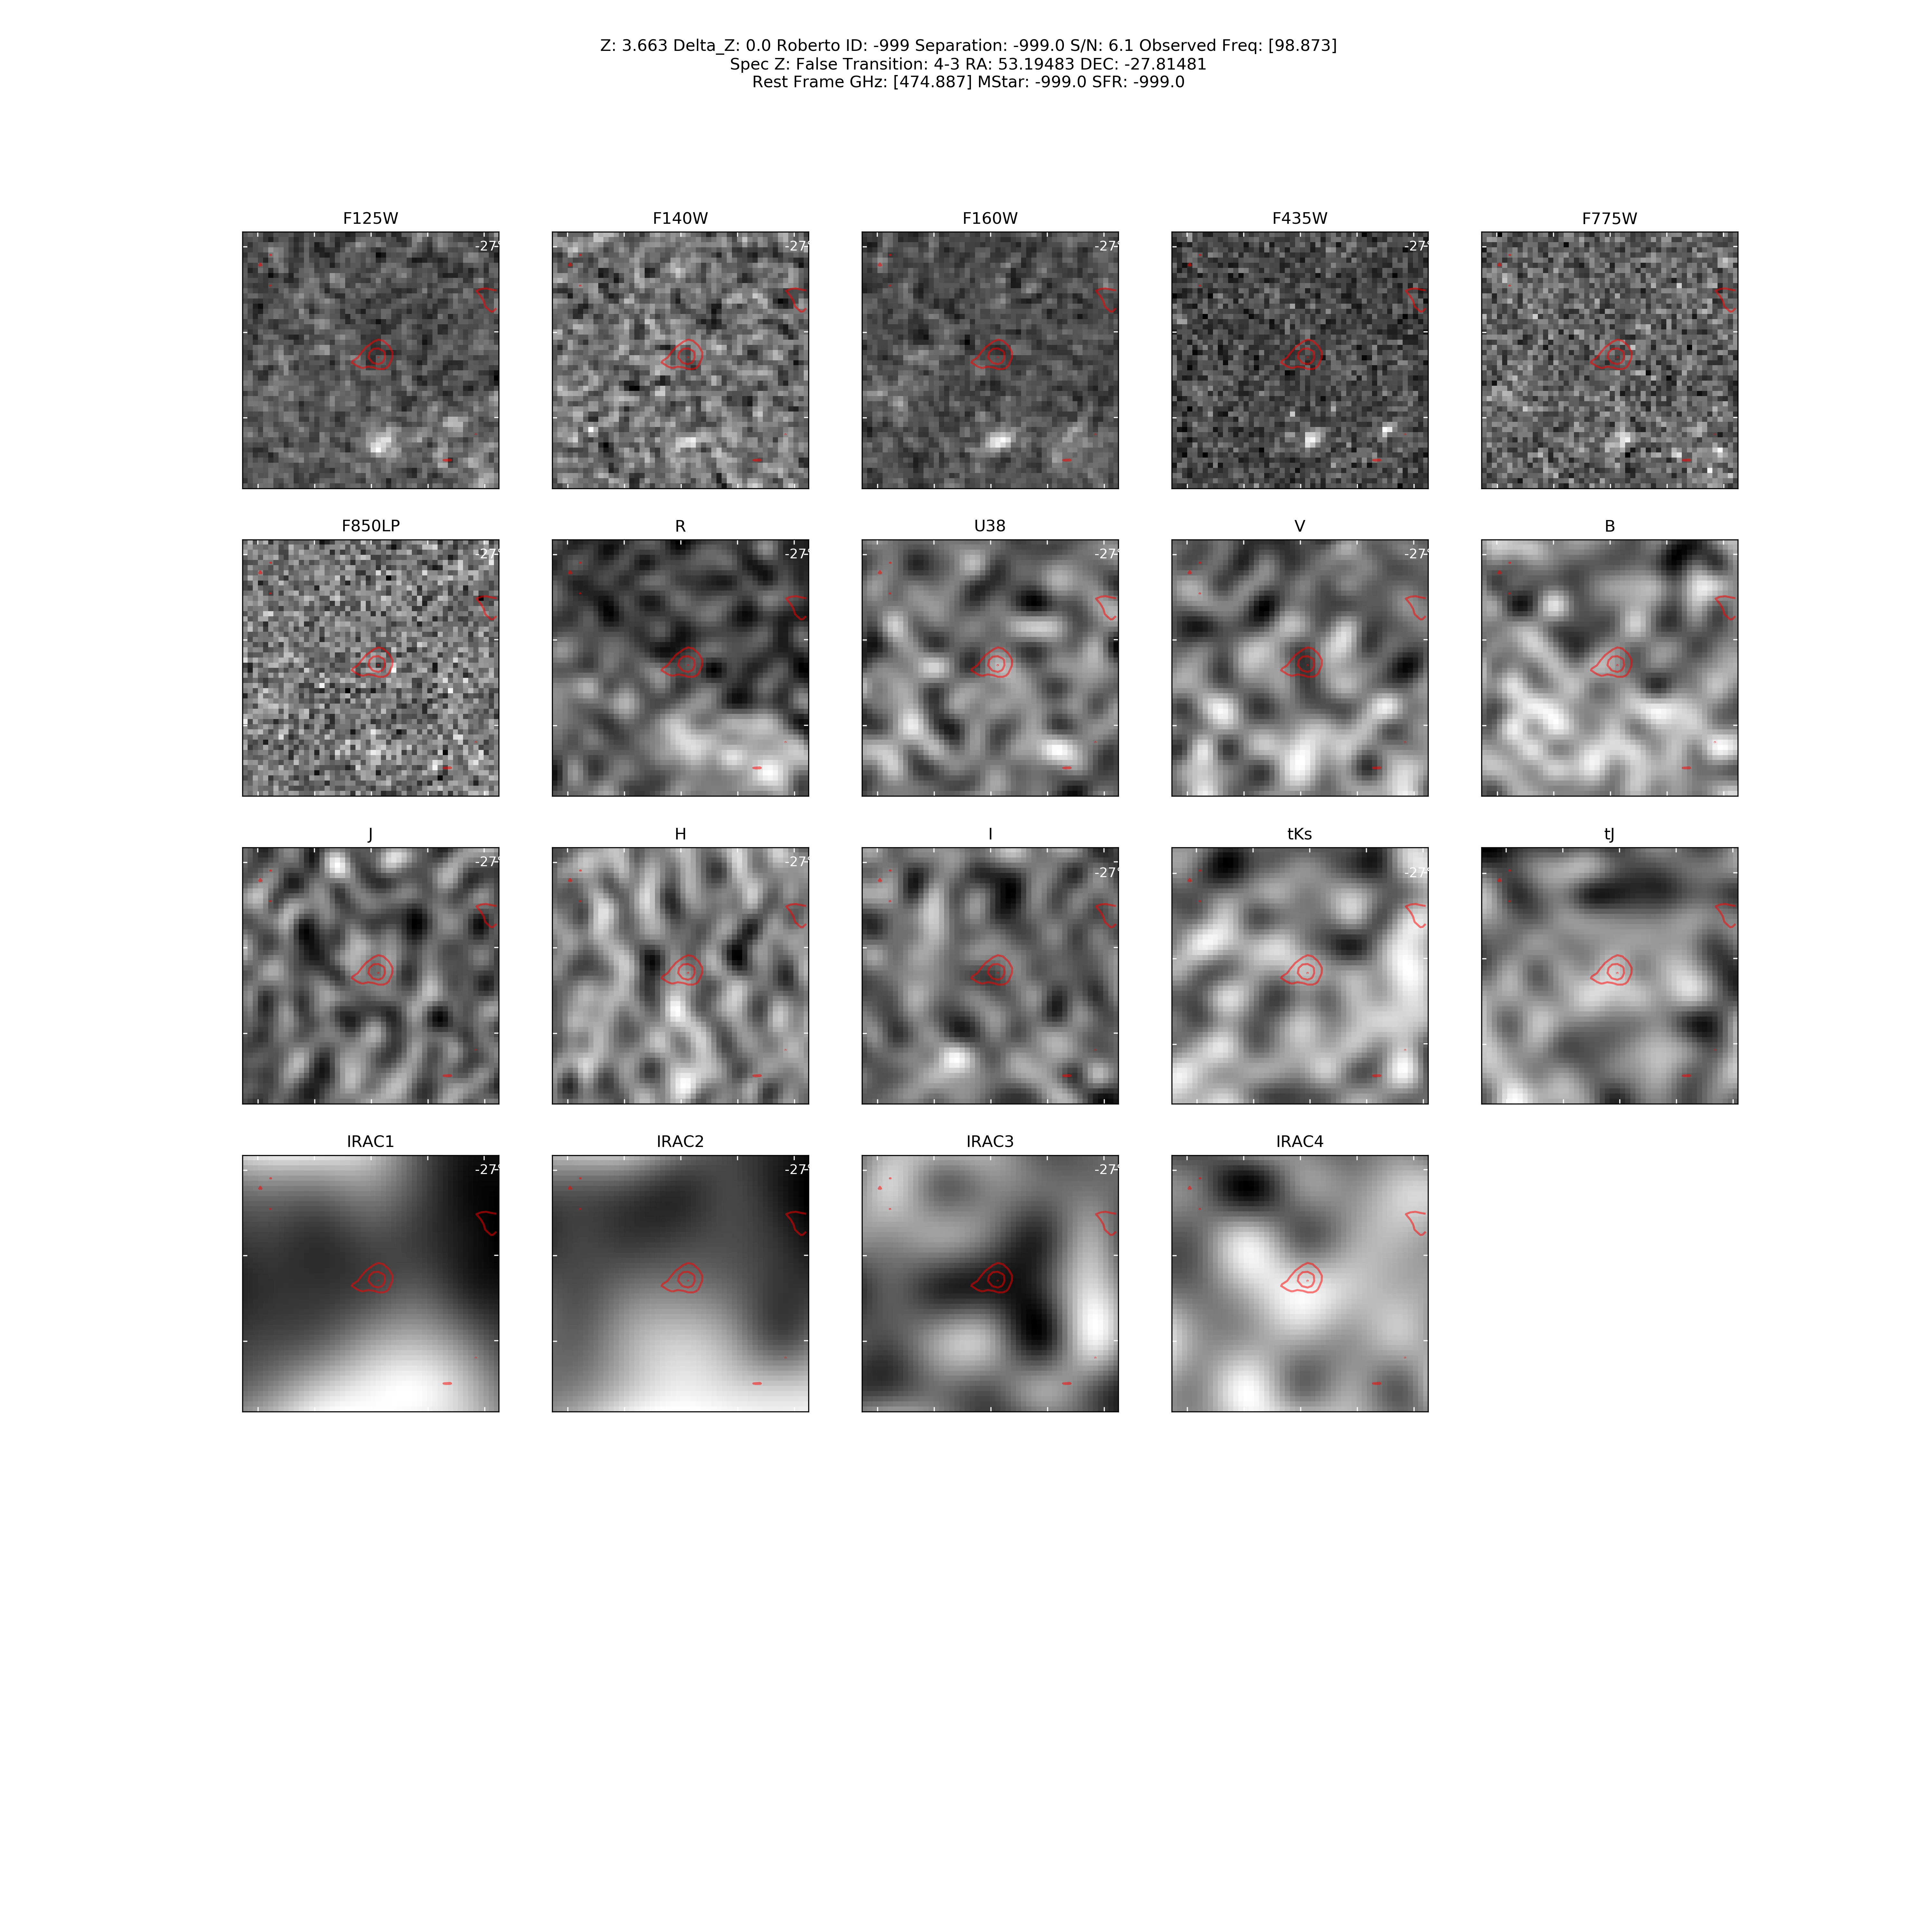
\includegraphics[width=160mm]{Matched/ASPECS_Cutout_5.png}
\caption{ID.6. Same contours and cutout size as for \ref{fig:Match_One}.}
\label{fig:Match_Five}
\end{figure}

\begin{figure}[tbp]
\centering 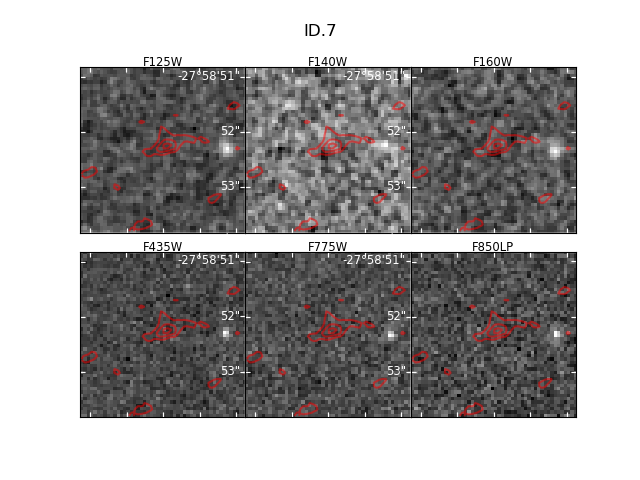
\includegraphics[width=160mm]{Matched/ASPECS_Cutout_6.png}
\caption{ID.7. Same contours and cutout size as for \ref{fig:Match_One}.}
\label{fig:Match_Three}
\end{figure}

\begin{figure}[tbp]
\centering 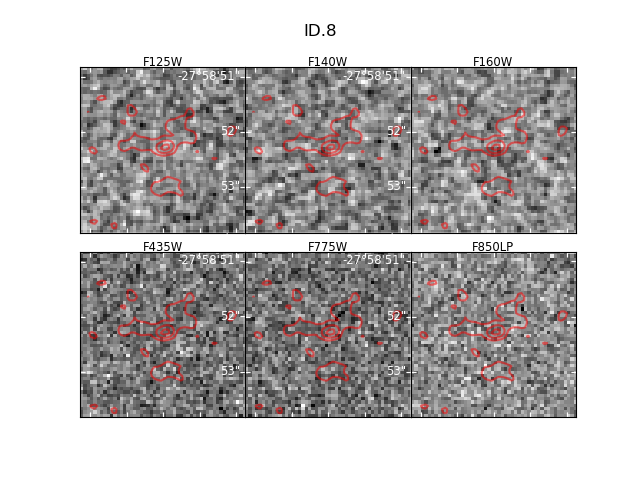
\includegraphics[width=160mm]{Matched/ASPECS_Cutout_7.png}
\caption{ID.8. Same contours and cutout size as for \ref{fig:Match_One}.}
\label{fig:Match_Three}
\end{figure}

\begin{figure}[tbp]
\centering 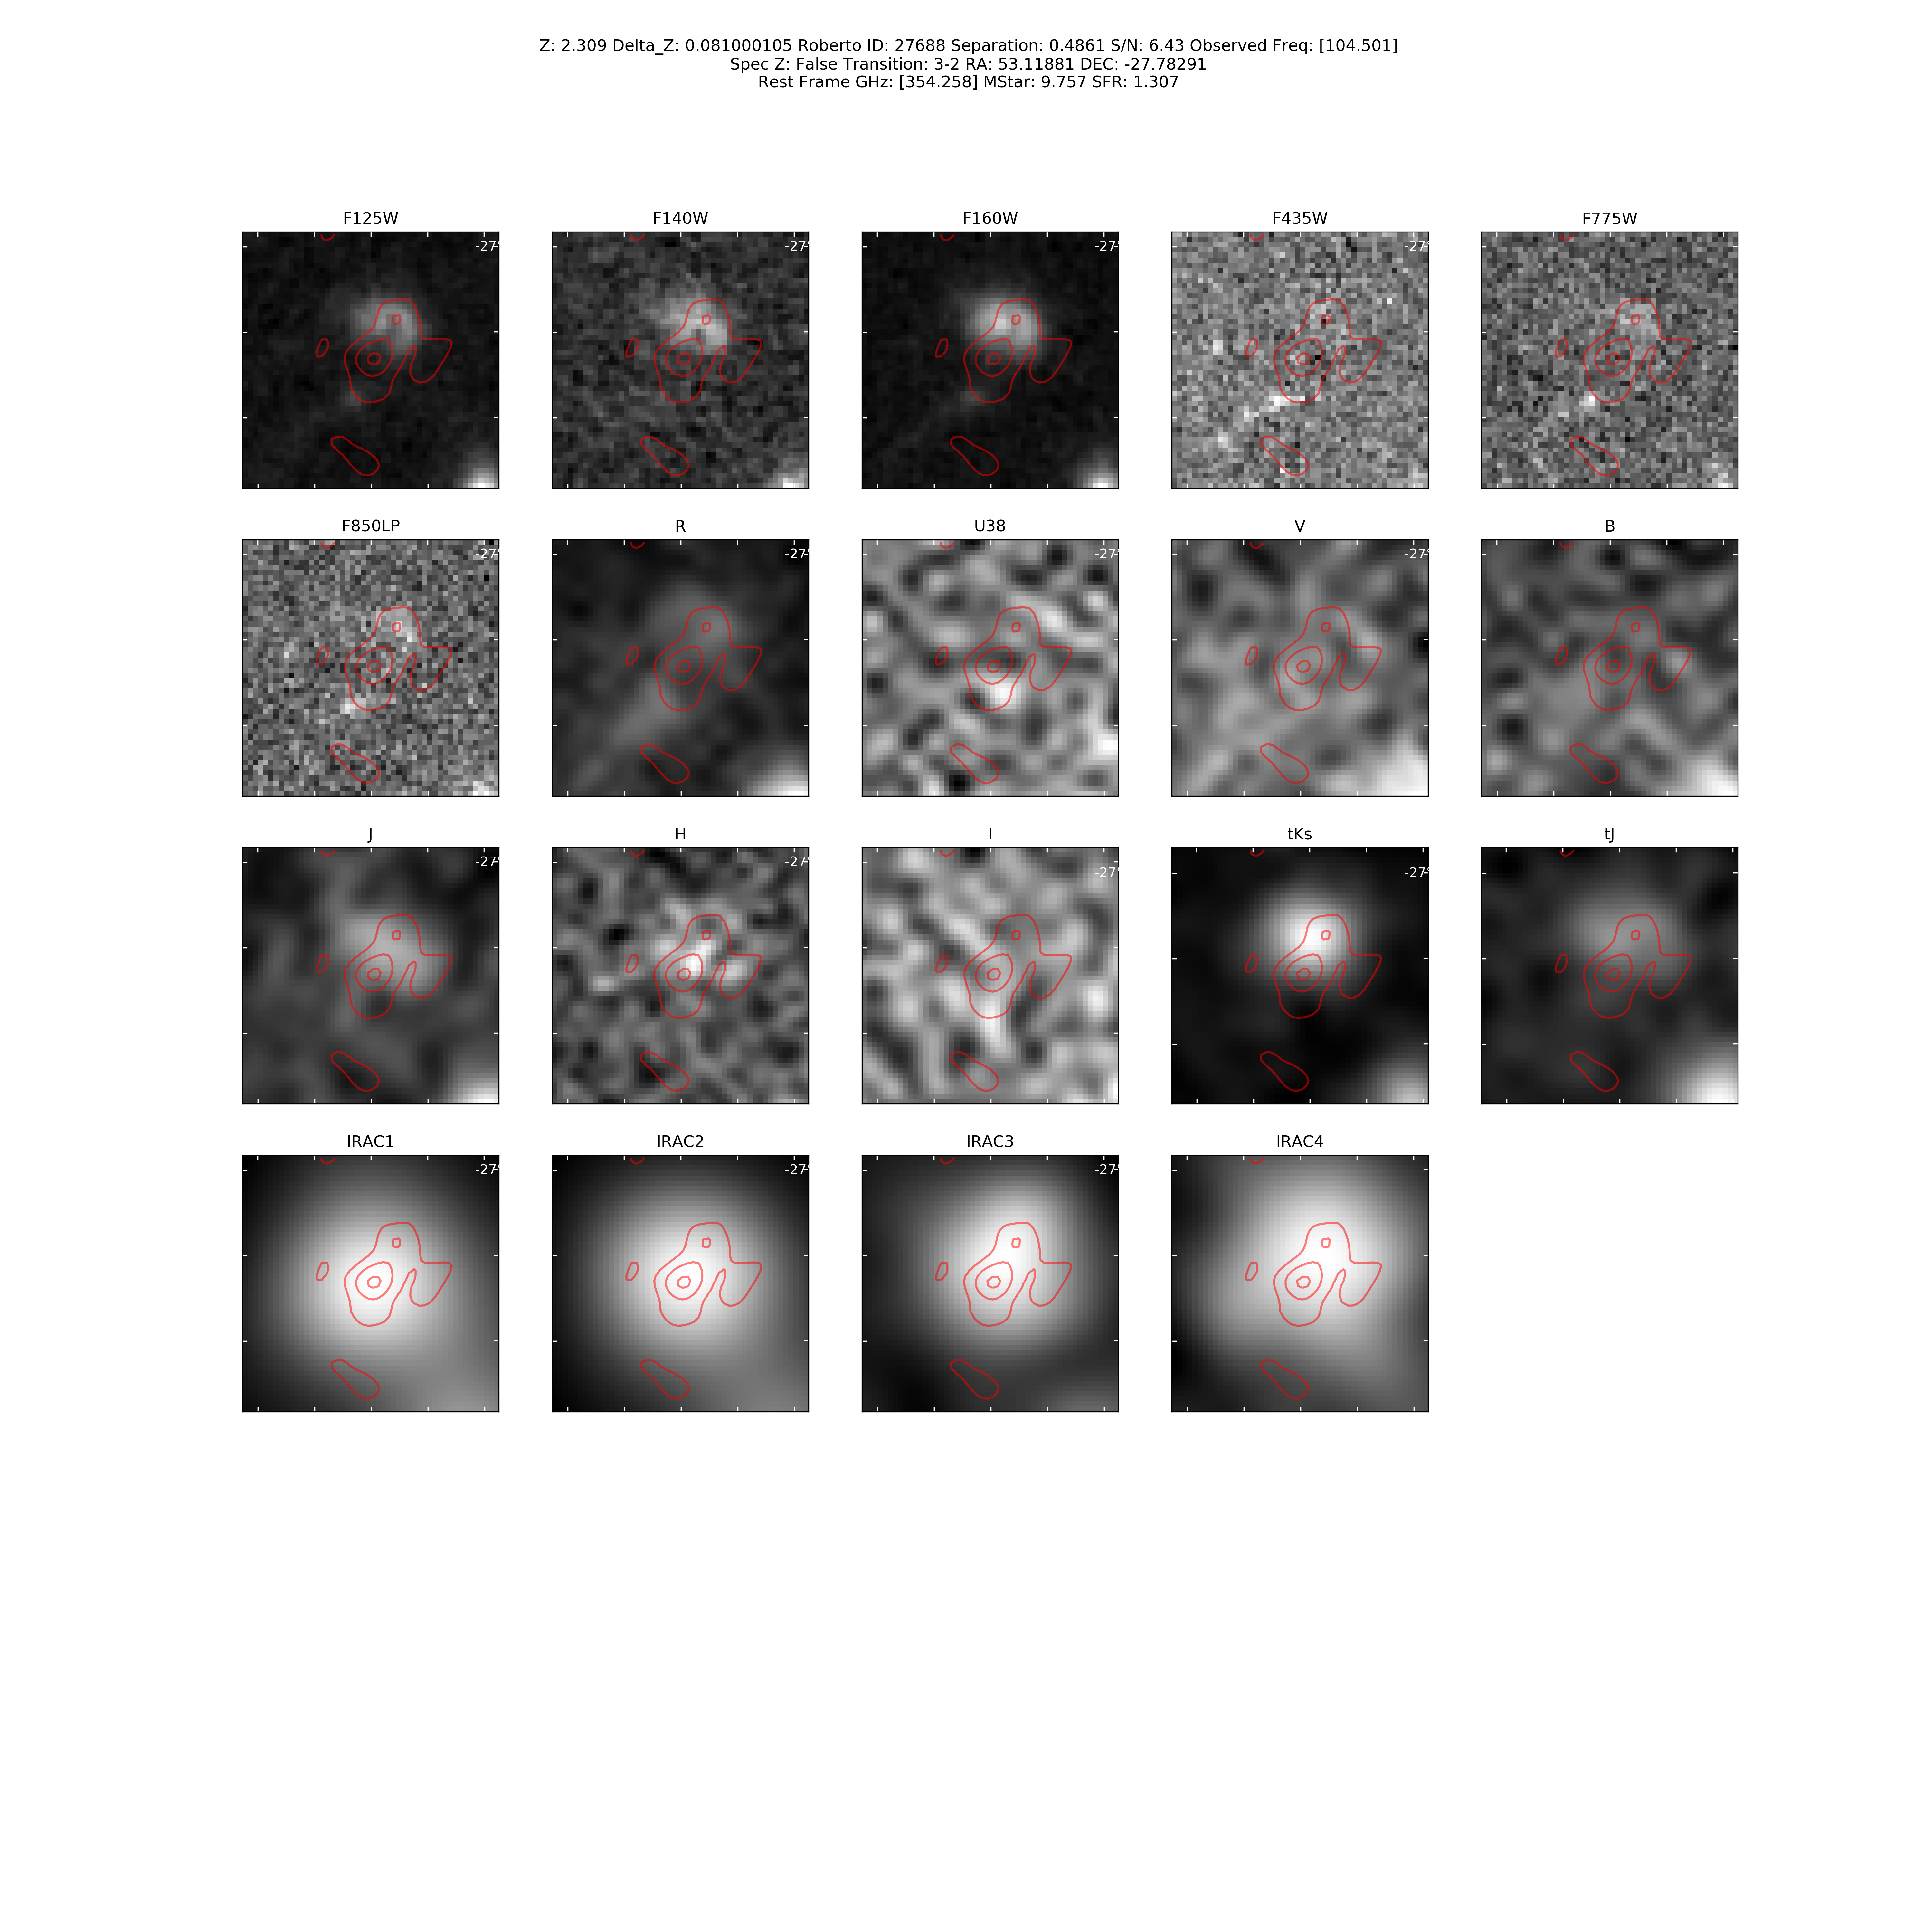
\includegraphics[width=160mm]{Matched/ASPECS_Cutout_8.png}
\caption{ID.9. Same contours and cutout size as for \ref{fig:Match_One}.}
\label{fig:Match_Three}
\end{figure}

\begin{figure}[tbp]
\centering 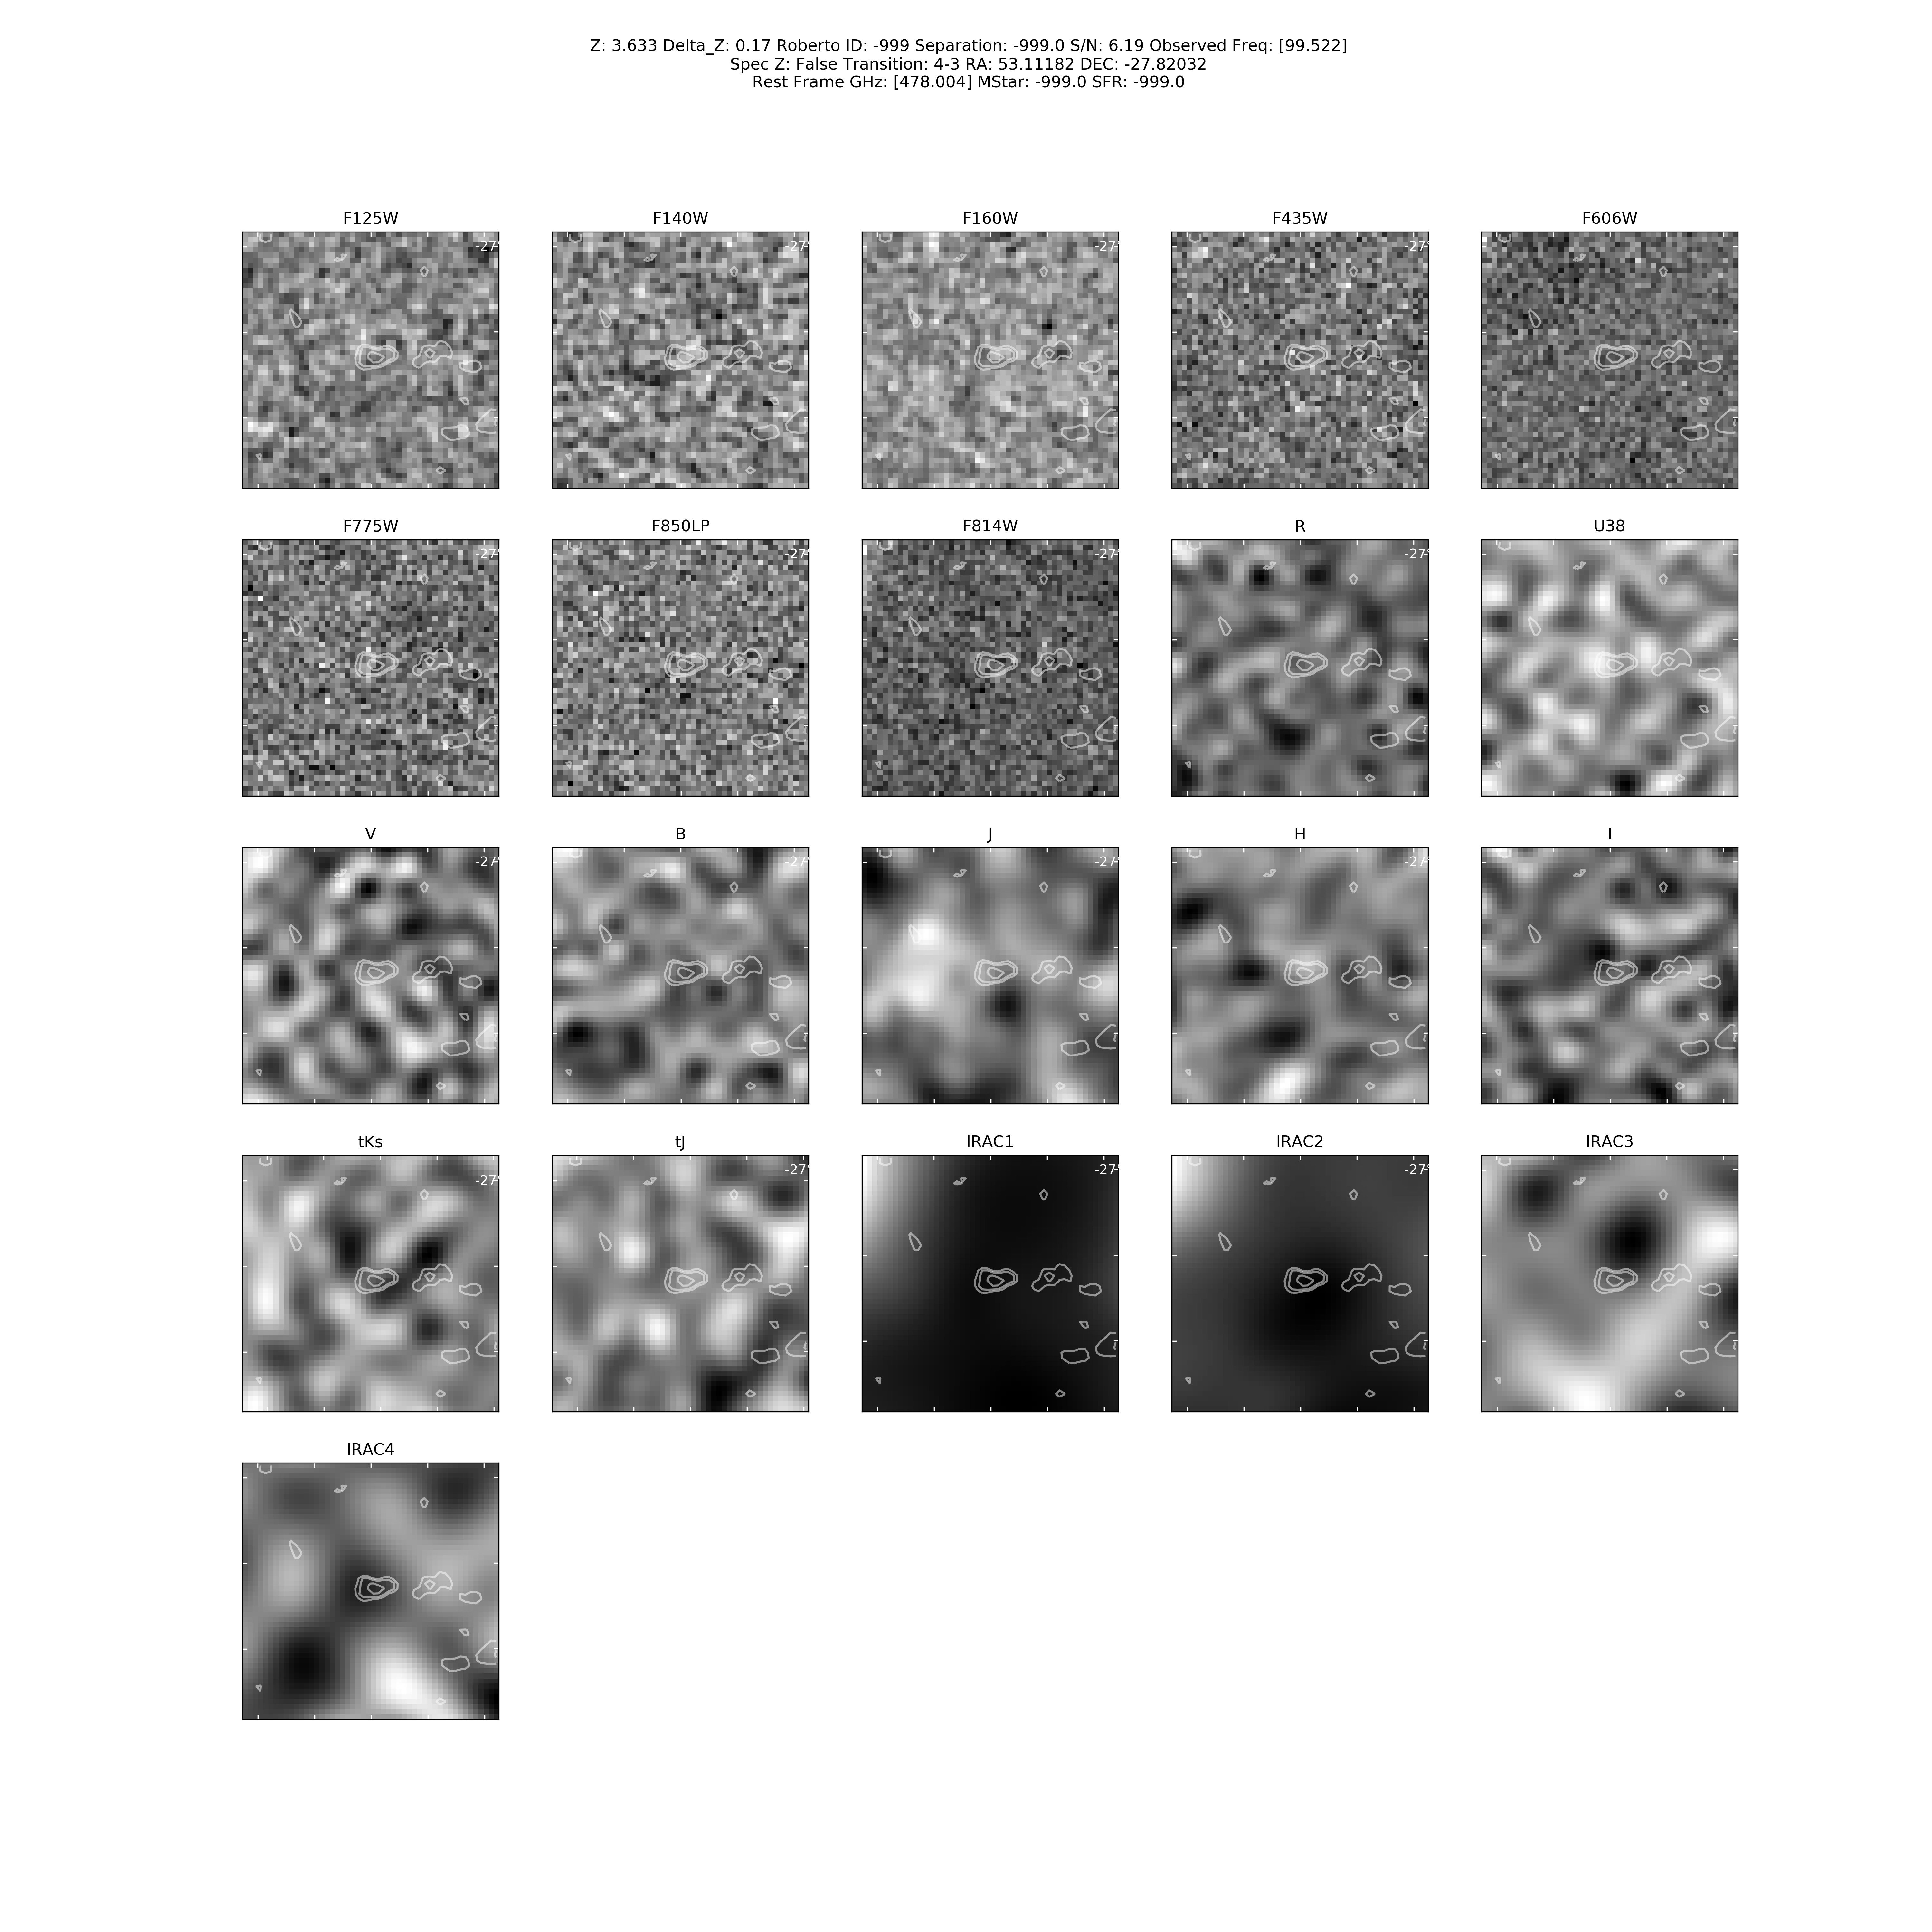
\includegraphics[width=160mm]{Matched/ASPECS_Cutout_9.png}
\caption{ID.10. Same contours and cutout size as for \ref{fig:Match_One}.}
\label{fig:Match_Three}
\end{figure}


\begin{figure}[tbp]
\centering 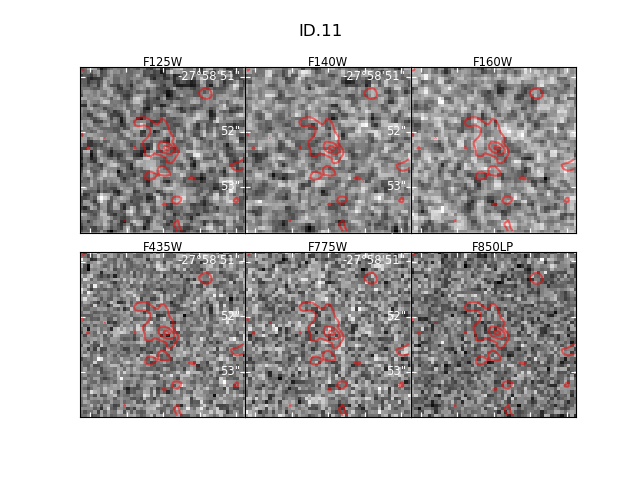
\includegraphics[width=160mm]{Matched/ASPECS_Cutout_10.png}
\caption{ID.11. Same contours and cutout size as for \ref{fig:Match_One}.}
\label{fig:Match_Three}
\end{figure}

\begin{figure}[tbp]
\centering 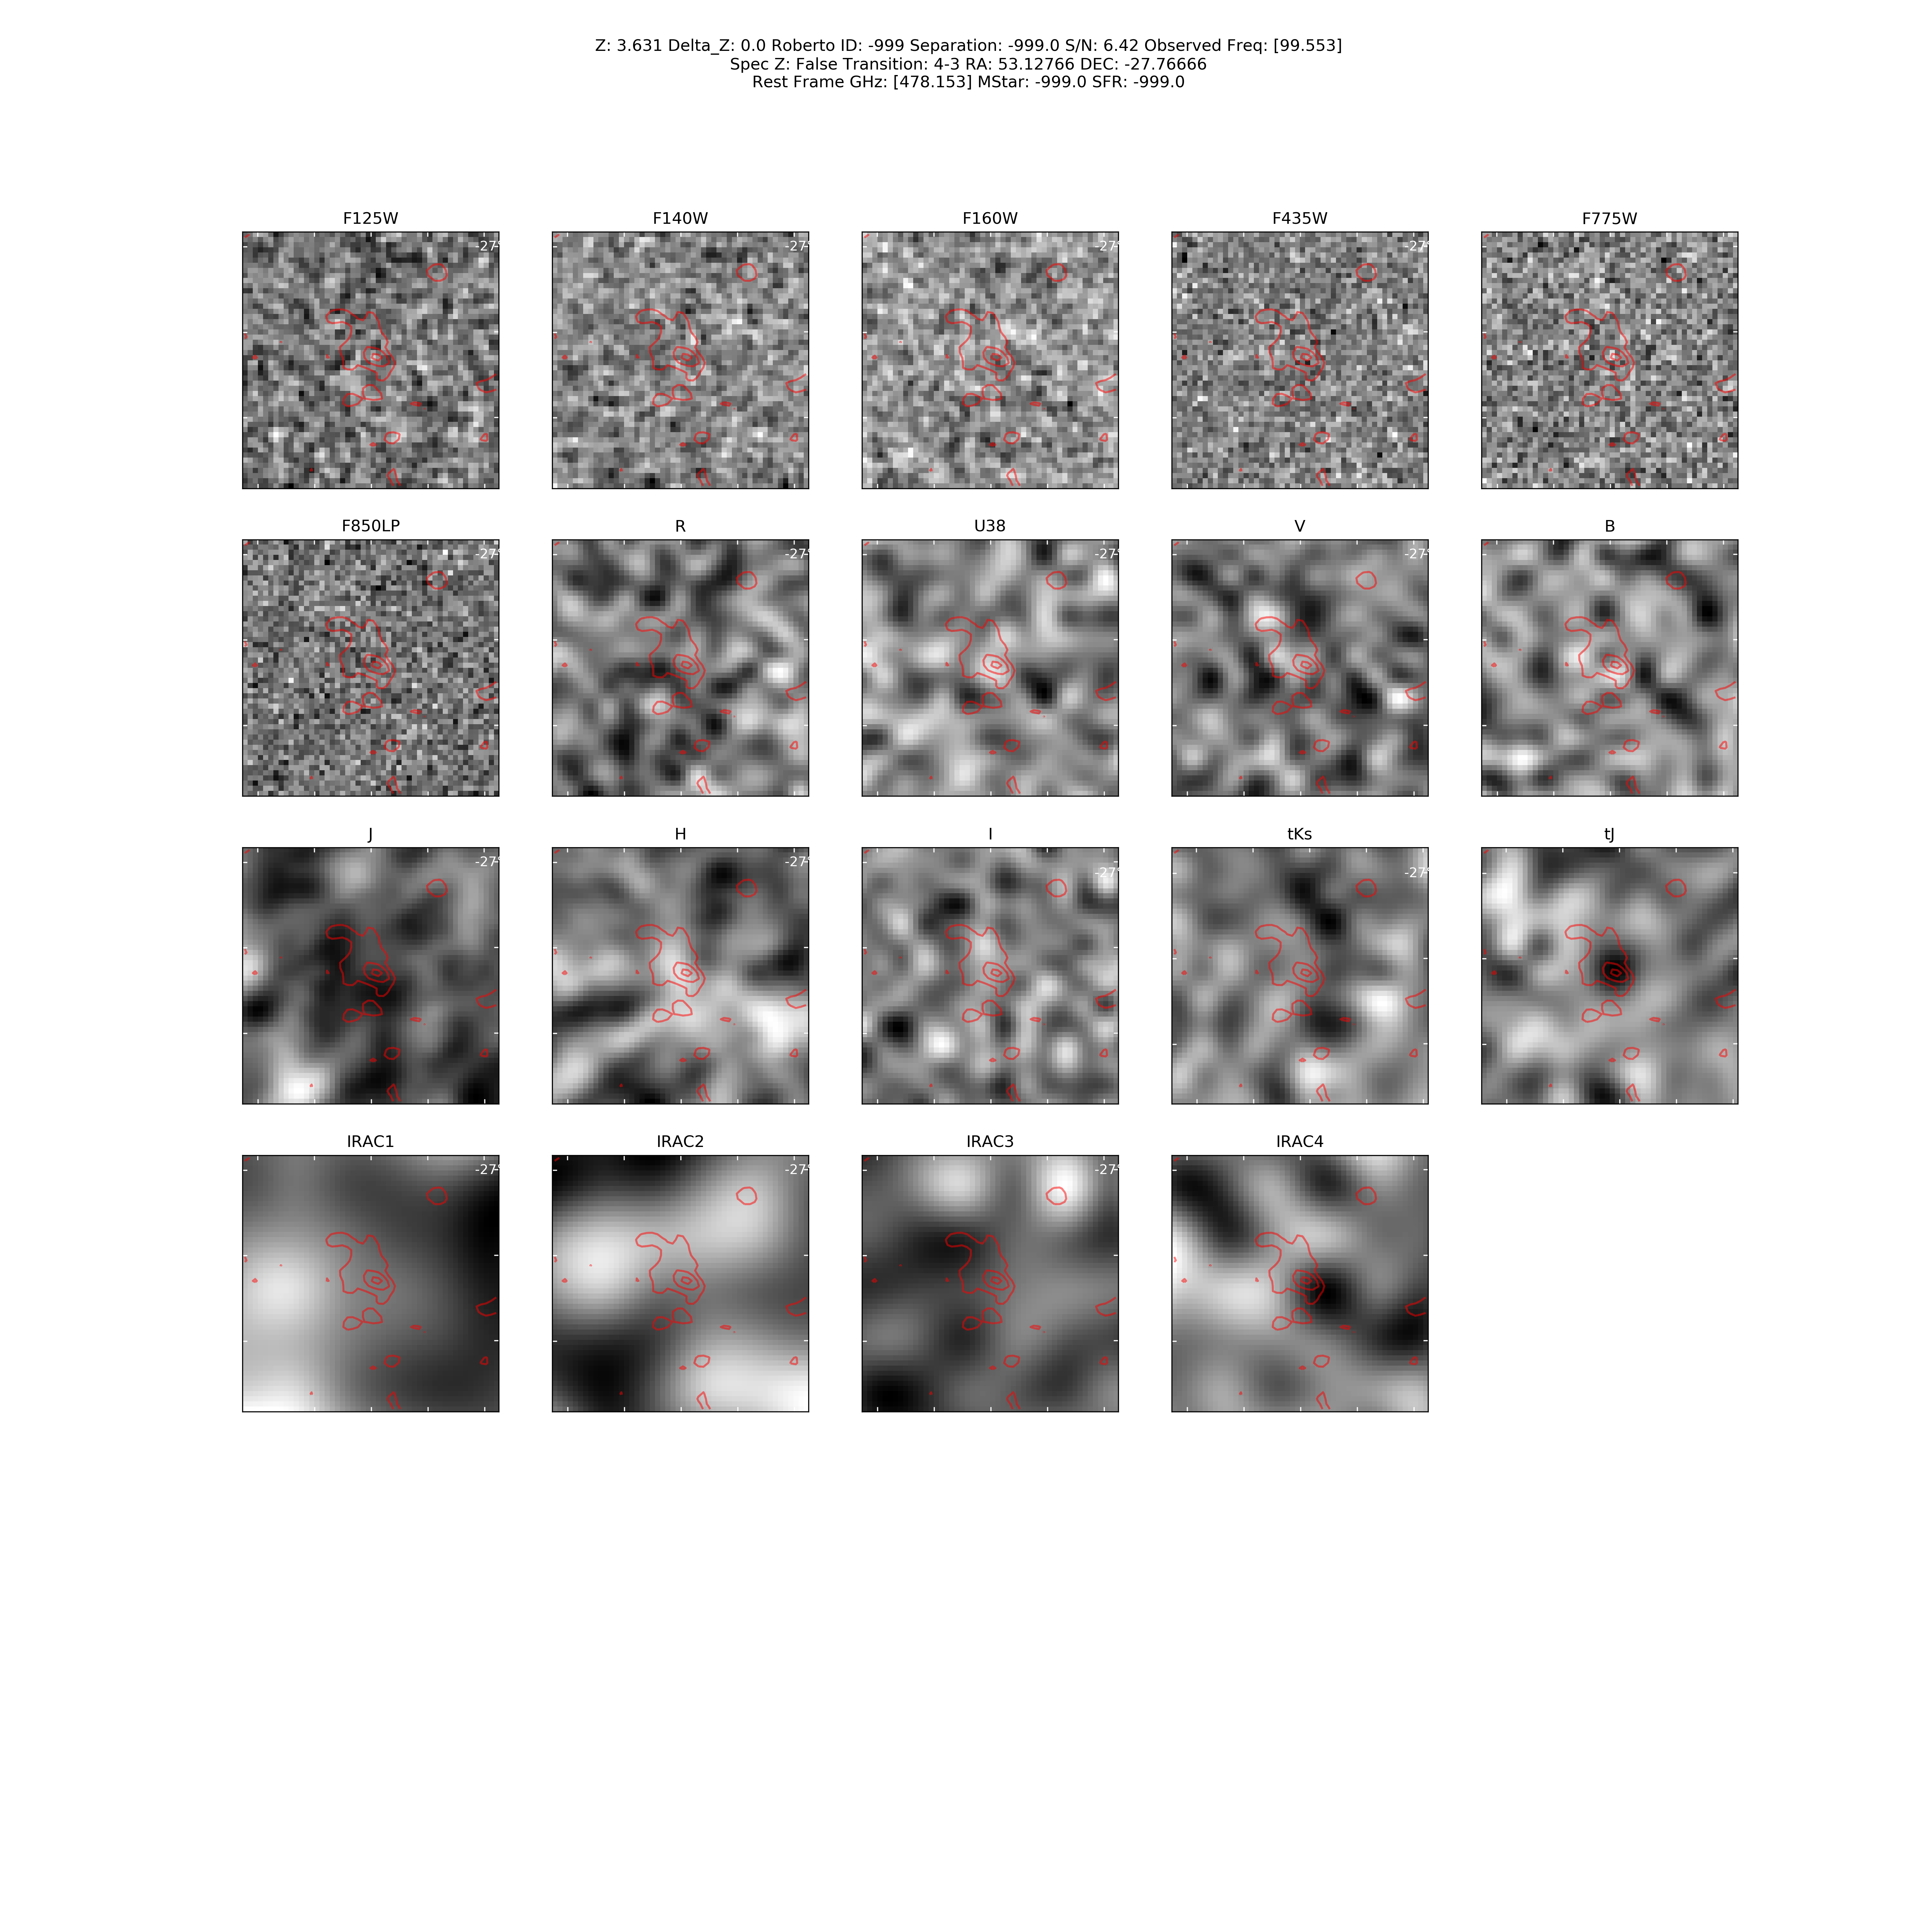
\includegraphics[width=160mm]{Matched/ASPECS_Cutout_11.png}
\caption{ID.12. Same contours and cutout size as for \ref{fig:Match_One}.}
\label{fig:Match_Three}
\end{figure}

\begin{figure}[tbp]
\centering 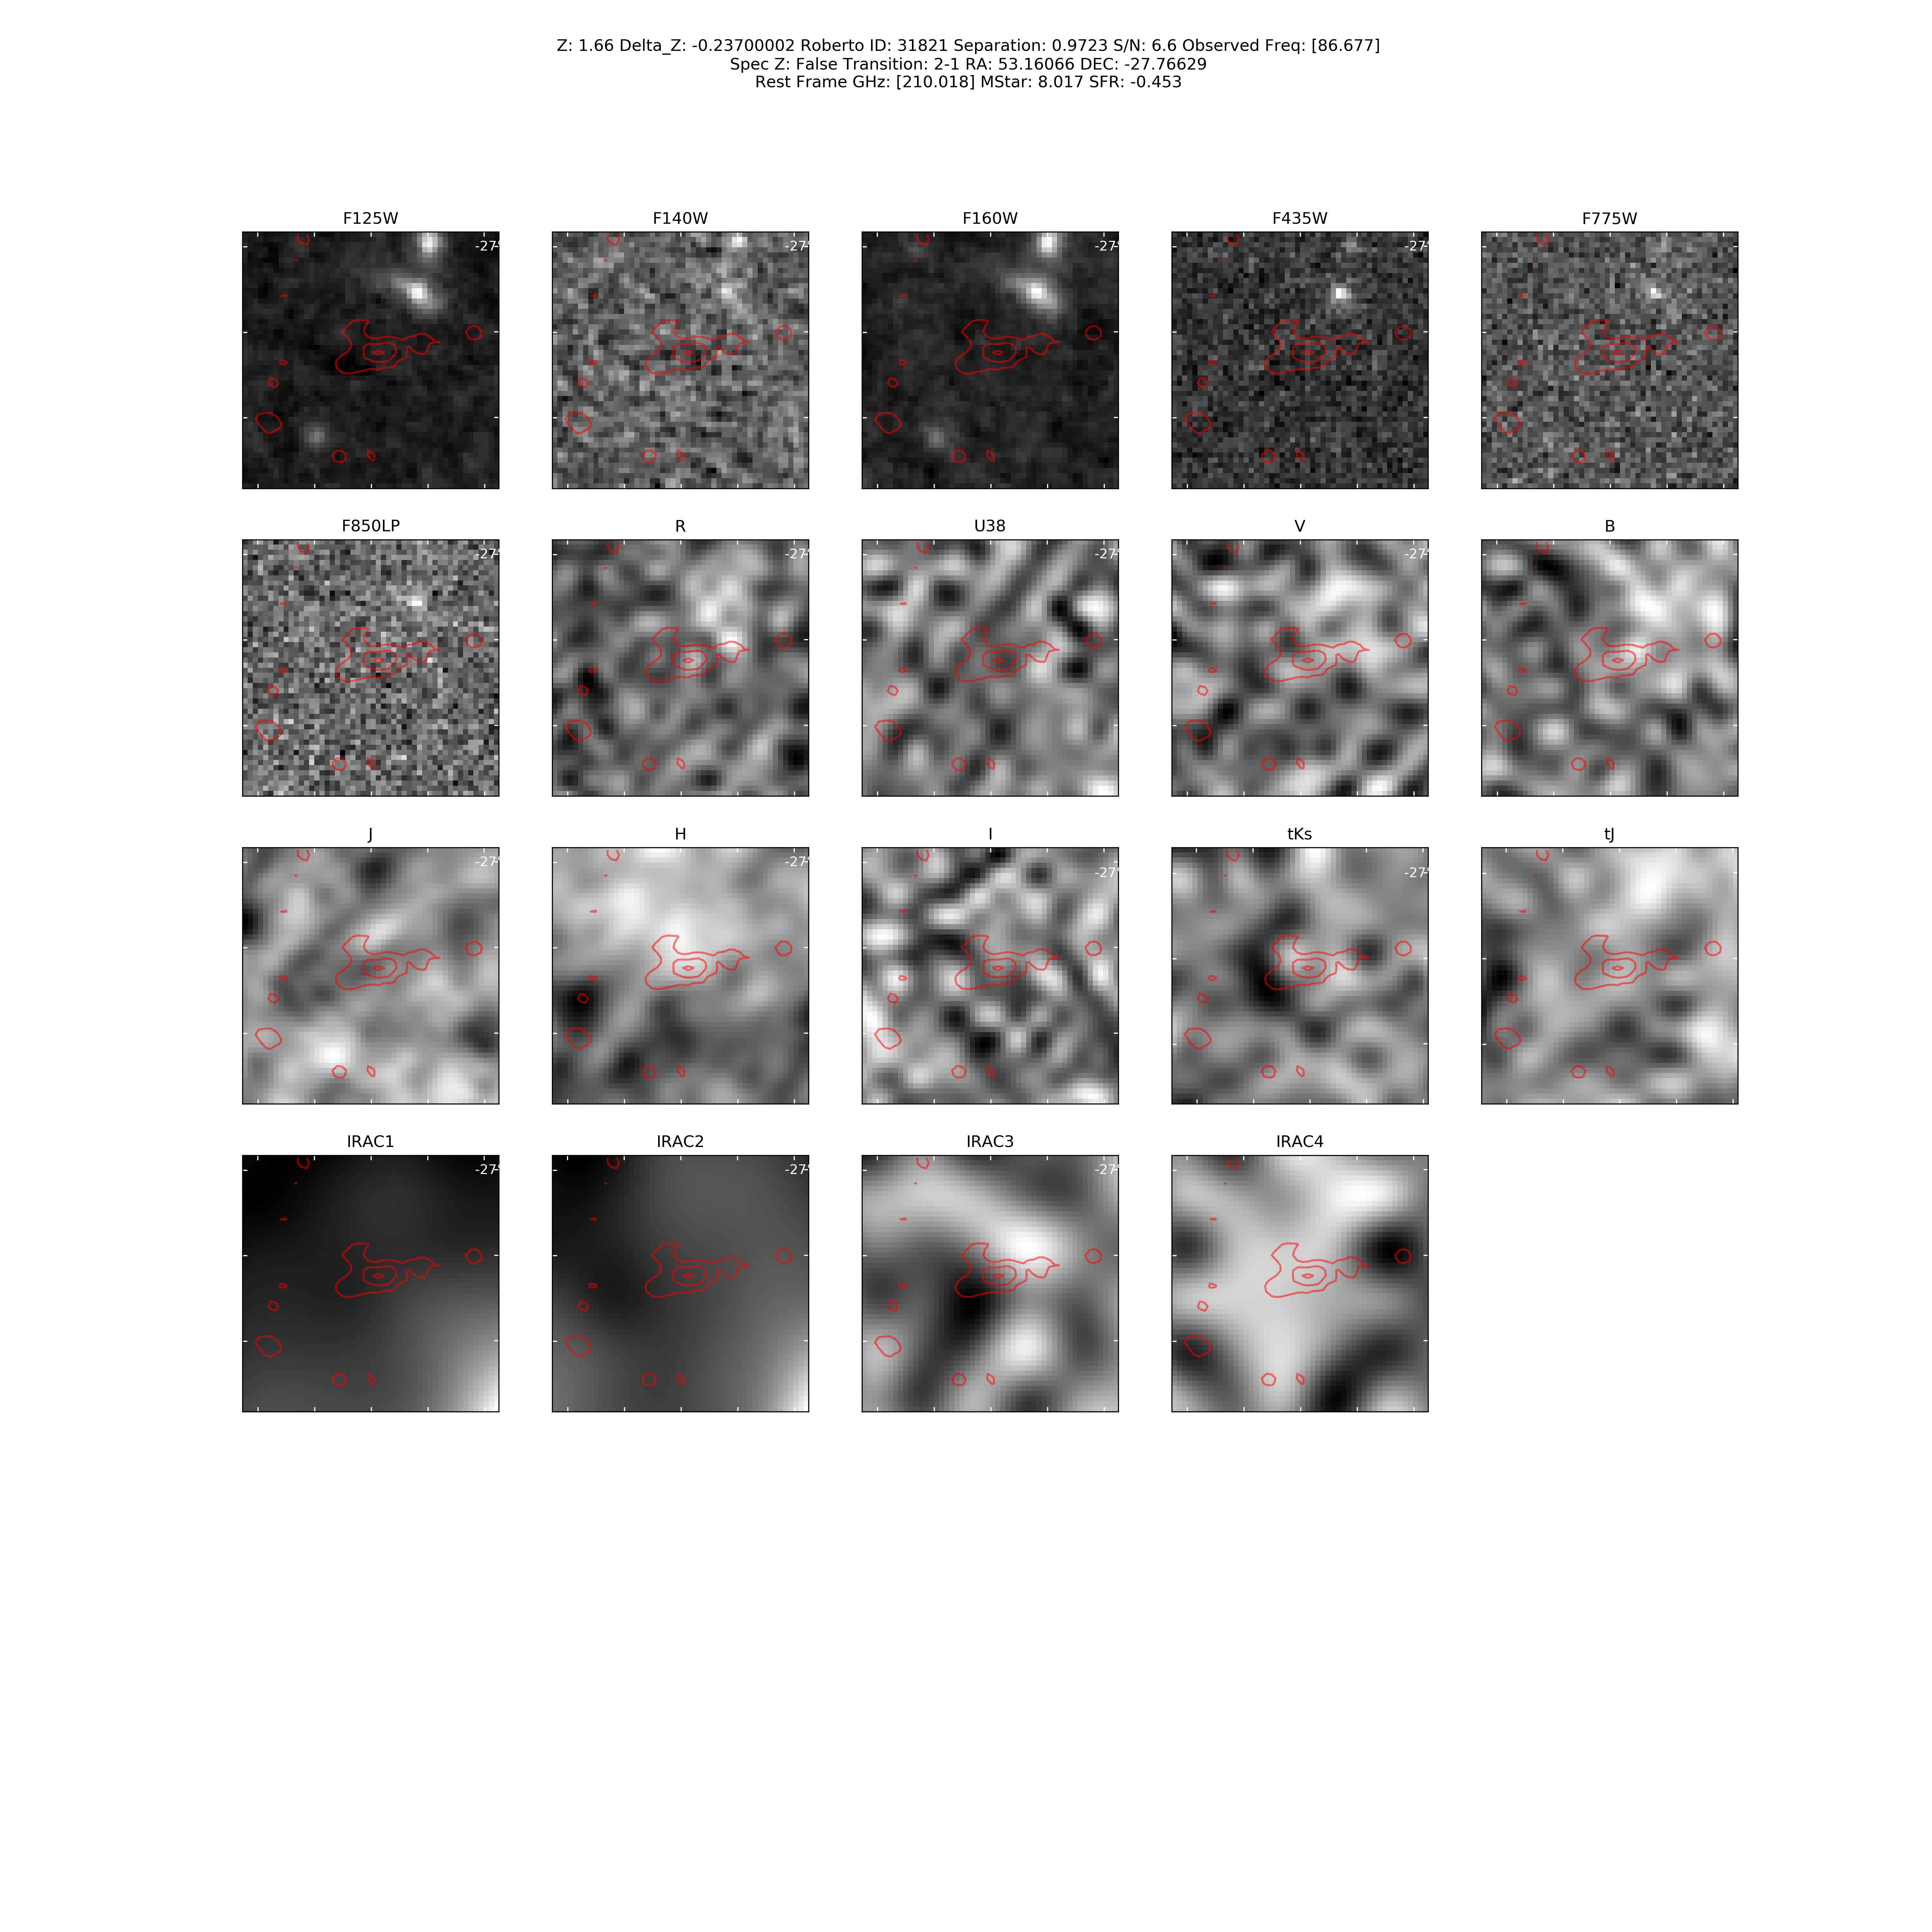
\includegraphics[width=160mm]{Matched/ASPECS_Cutout_12.png}
\caption{ID.13. Same contours and cutout size as for \ref{fig:Match_One}.}
\label{fig:Match_Three}
\end{figure}

\begin{figure}[tbp]
\centering 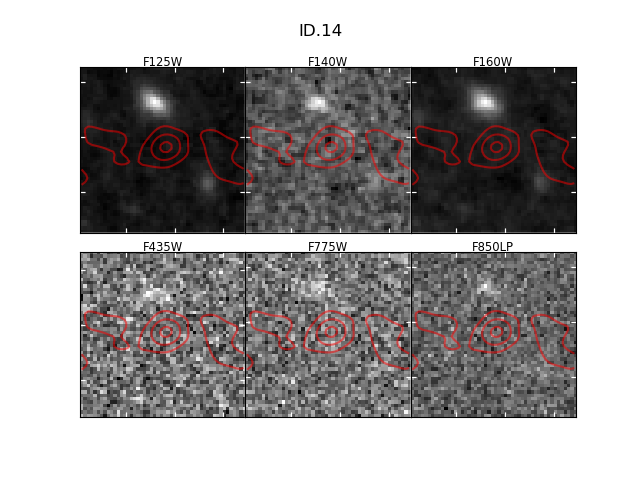
\includegraphics[width=160mm]{Matched/ASPECS_Cutout_13.png}
\caption{ID.14. Same contours and cutout size as for \ref{fig:Match_One}.}
\label{fig:Match_Three}
\end{figure}

\begin{figure}[tbp]
\centering 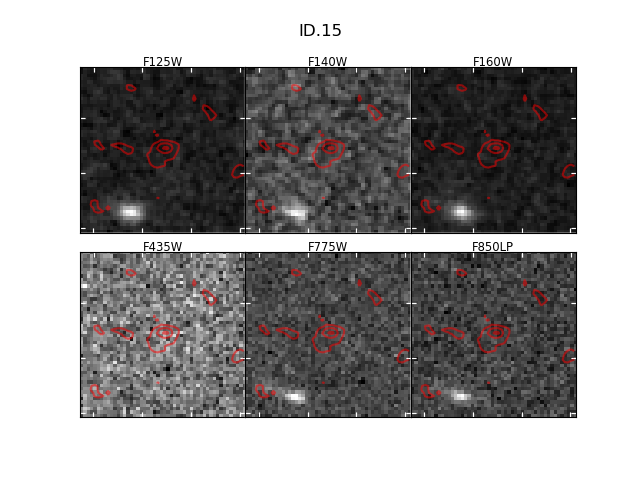
\includegraphics[width=160mm]{Matched/ASPECS_Cutout_14.png}
\caption{ID.15. Same contours and cutout size as for \ref{fig:Match_One}.}
\label{fig:Match_Three}
\end{figure}

\begin{figure}[tbp]
\centering 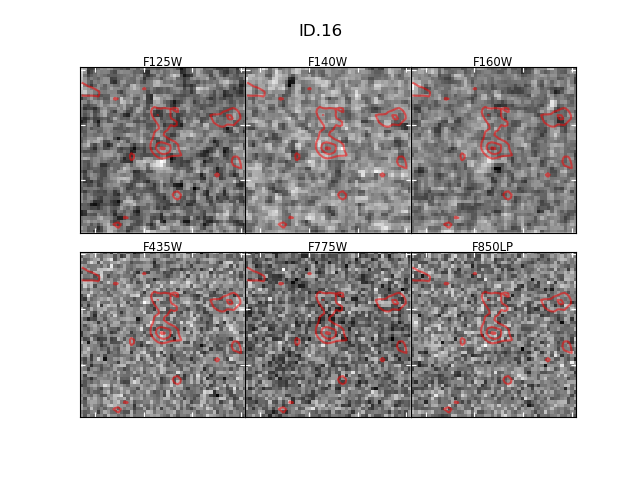
\includegraphics[width=160mm]{Matched/ASPECS_Cutout_15.png}
\caption{ID.16. Same contours and cutout size as for \ref{fig:Match_One}.}
\label{fig:Match_Three}
\end{figure}

\begin{figure}[tbp]
\centering 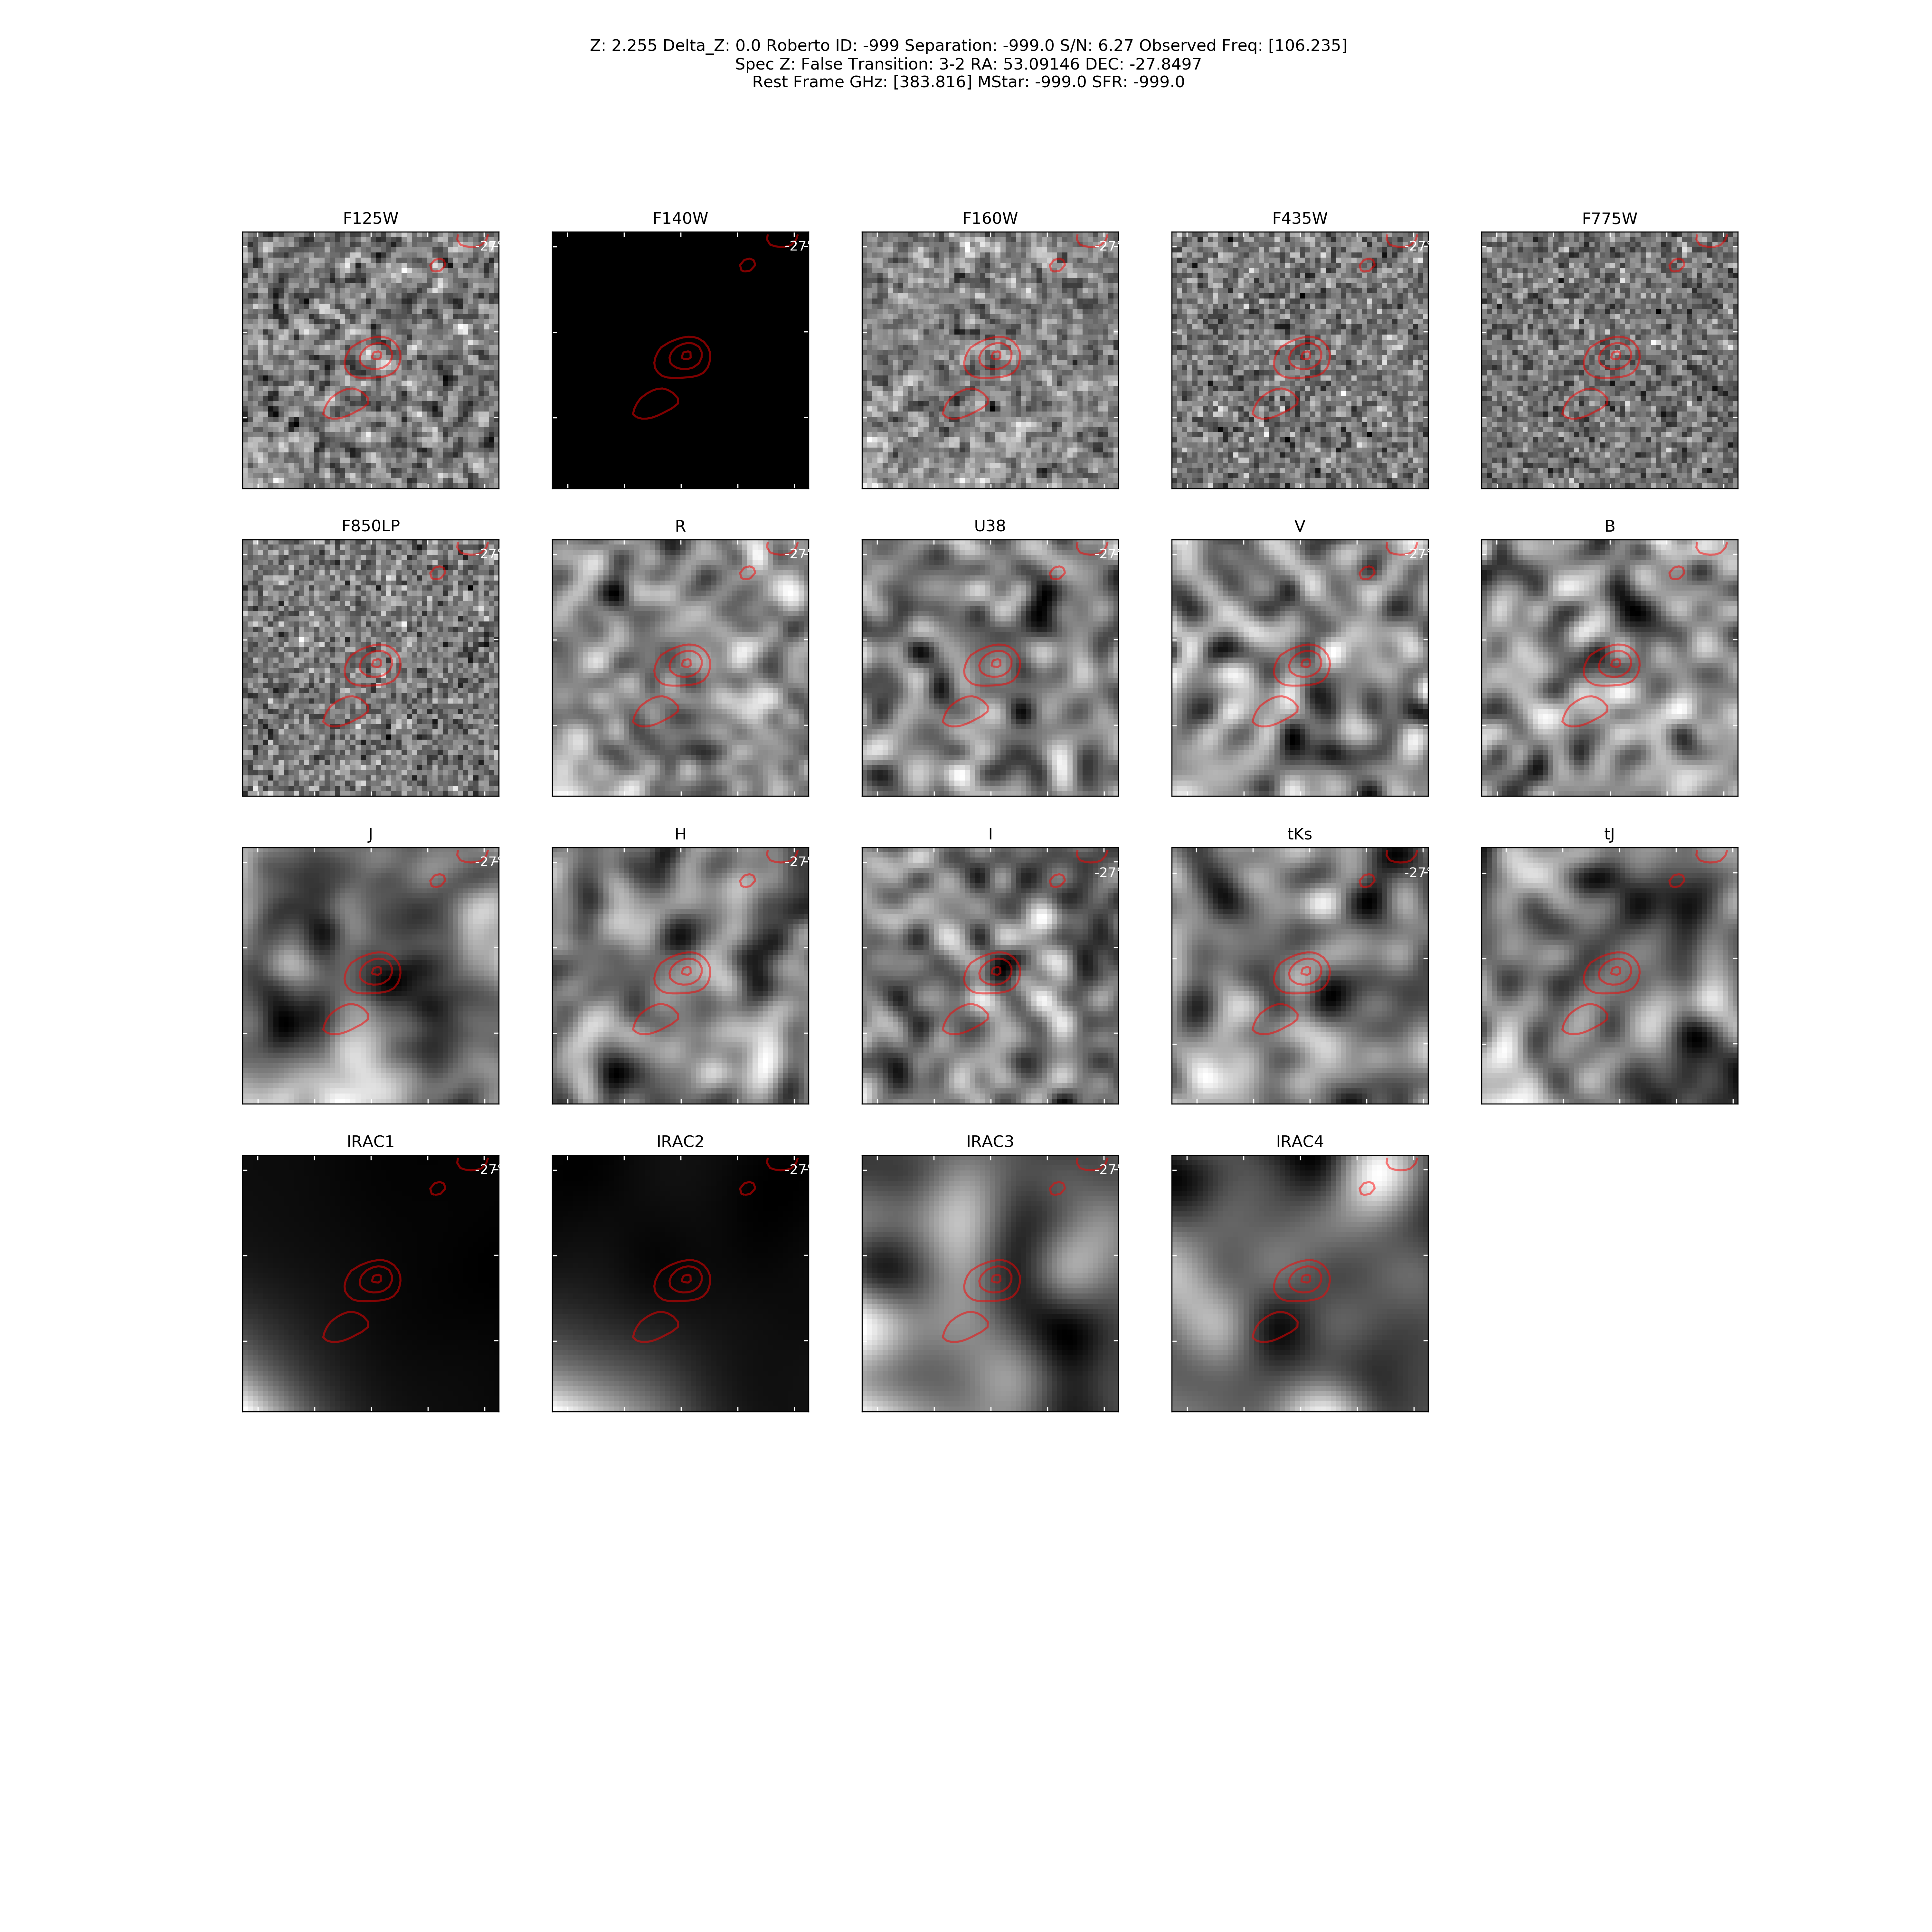
\includegraphics[width=160mm]{Matched/ASPECS_Cutout_16.png}
\caption{ID.17. Same contours and cutout size as for \ref{fig:Match_One}.}
\label{fig:Match_Three}
\end{figure}

\begin{figure}[tbp]
\centering 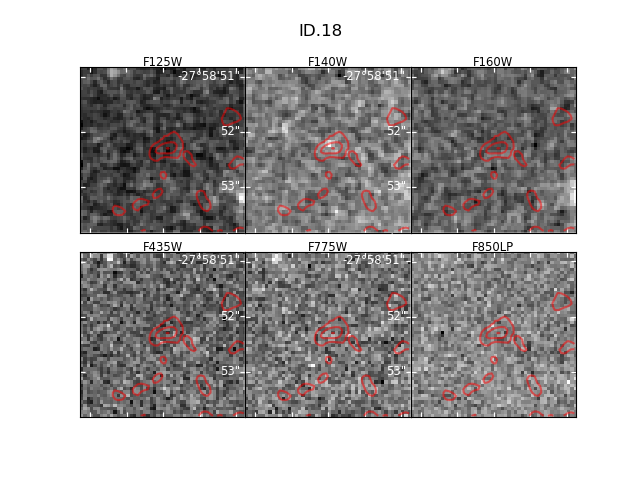
\includegraphics[width=160mm]{Matched/ASPECS_Cutout_17.png}
\caption{ID.18. Same contours and cutout size as for \ref{fig:Match_One}.}
\label{fig:Match_Three}
\end{figure}

\begin{figure}[tbp]
\centering 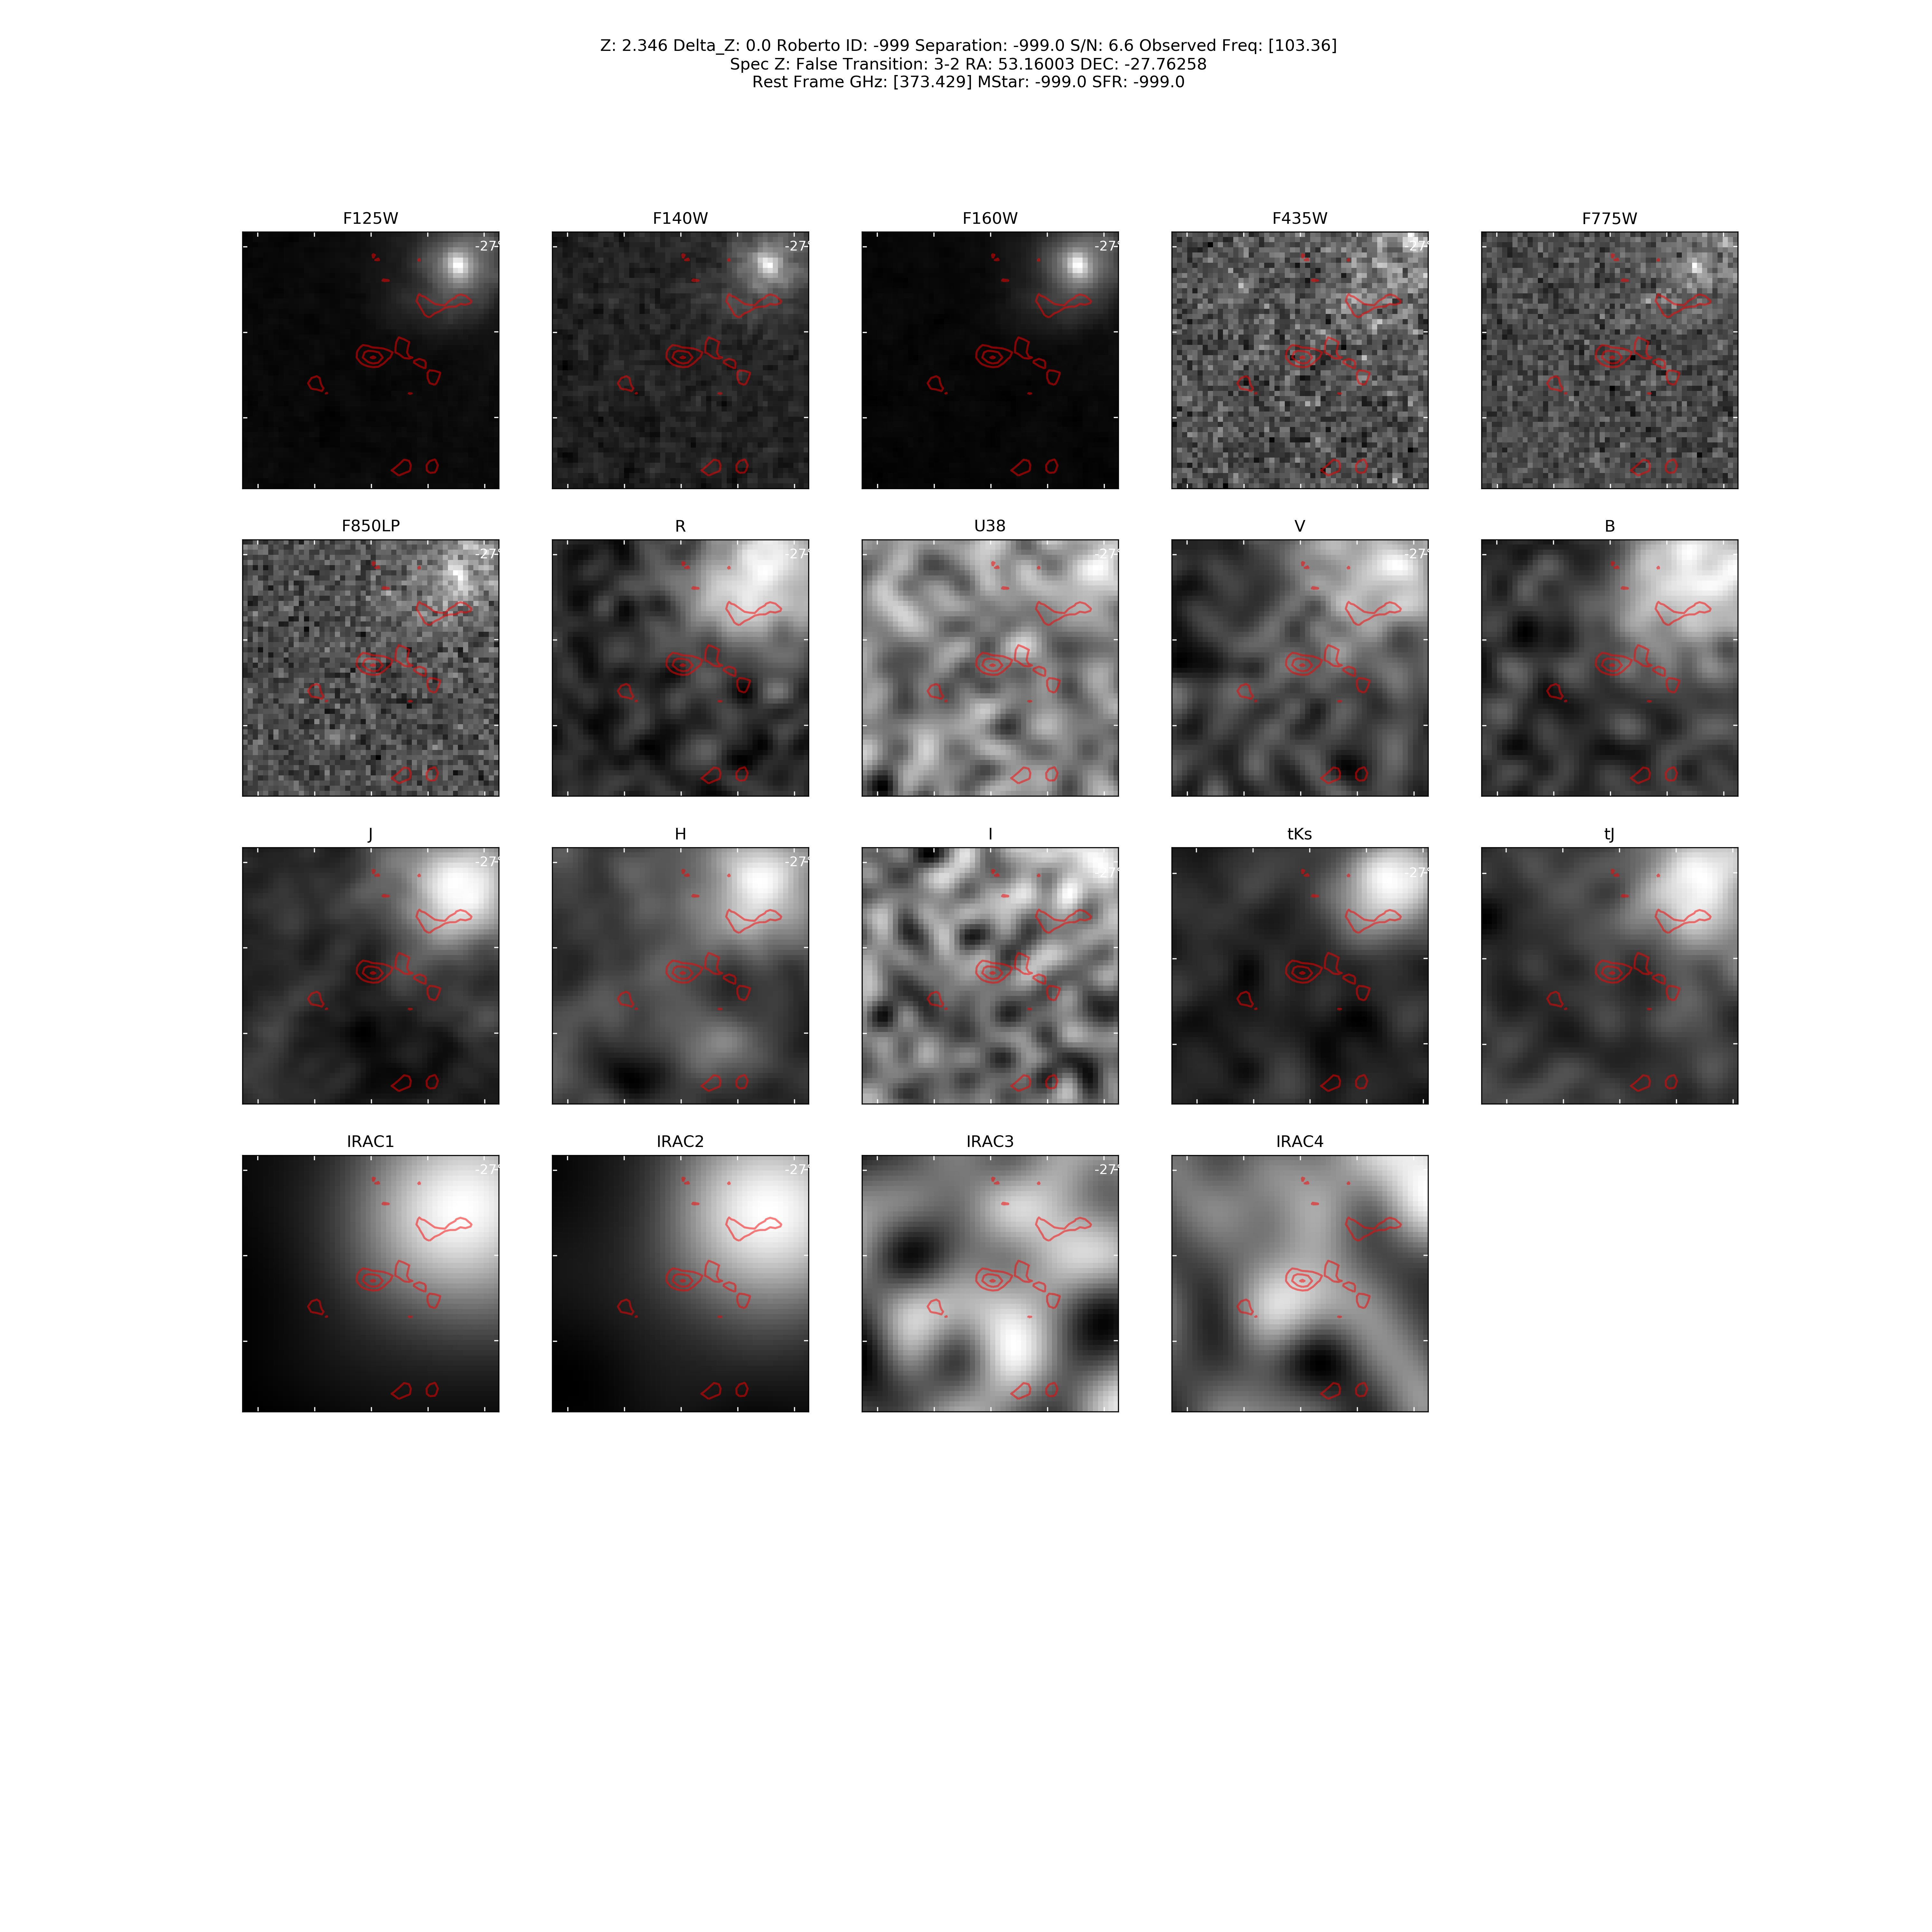
\includegraphics[width=160mm]{Matched/ASPECS_Cutout_18.png}
\caption{ID.19. Same contours and cutout size as for \ref{fig:Match_One}.}
\label{fig:Match_Three}
\end{figure}

\begin{figure}[tbp]
\centering 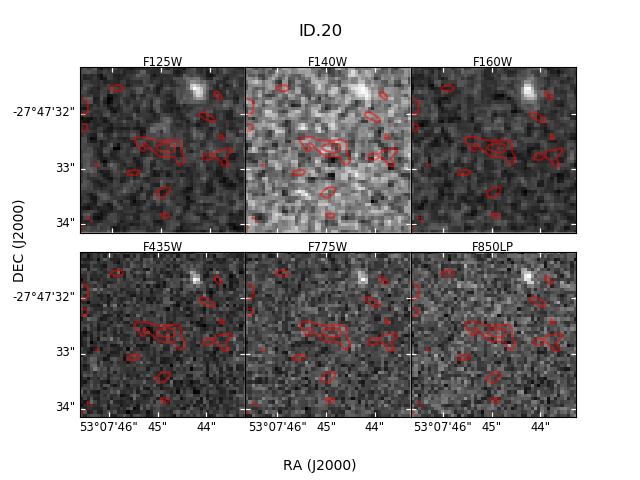
\includegraphics[width=160mm]{Matched/ASPECS_Cutout_19.png}
\caption{ID.20. Same contours and cutout size as for \ref{fig:Match_One}.}
\label{fig:Match_Three}
\end{figure}

\begin{figure}[tbp]
\centering 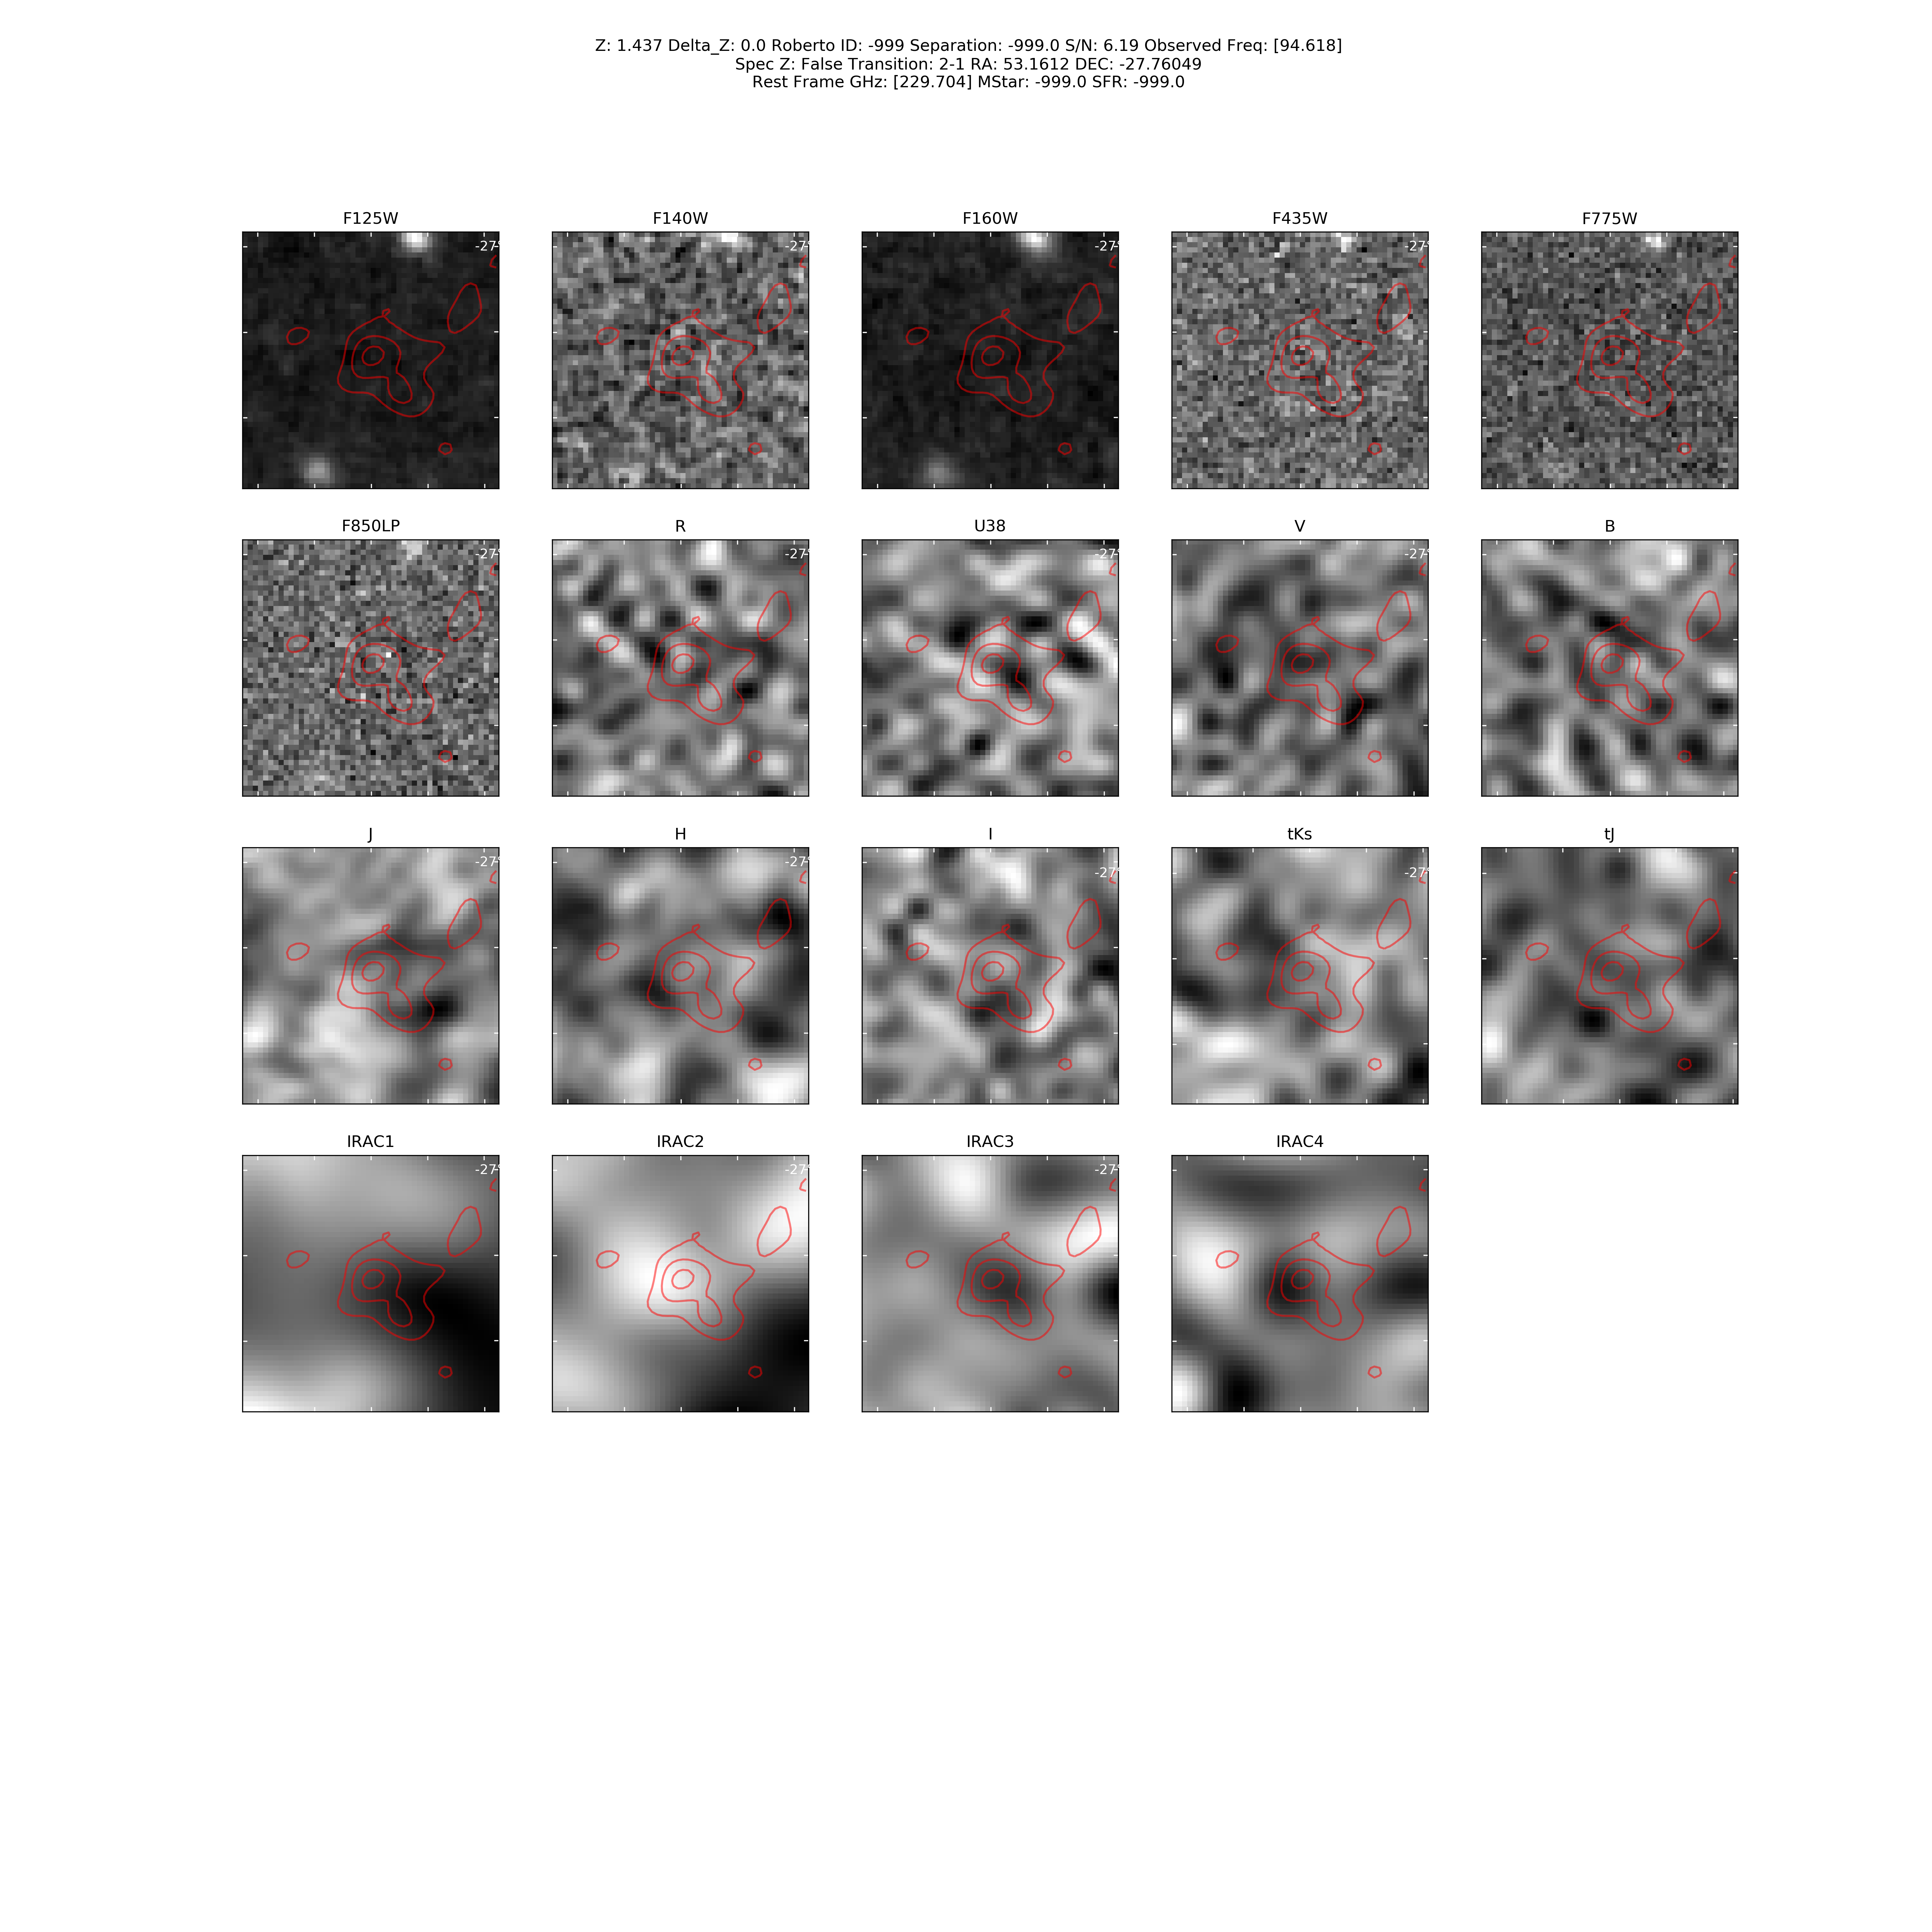
\includegraphics[width=160mm]{Matched/ASPECS_Cutout_20.png}
\caption{ID.21. Same contours and cutout size as for \ref{fig:Match_One}.}
\label{fig:Match_Three}
\end{figure}

\begin{figure}[tbp]
\centering 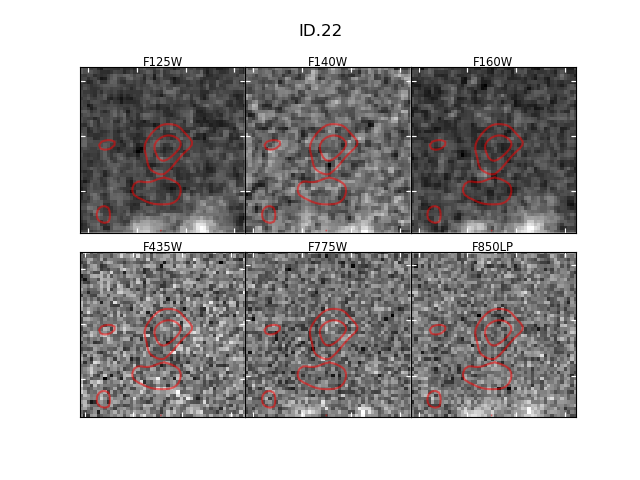
\includegraphics[width=160mm]{Matched/ASPECS_Cutout_21.png}
\caption{ID.22. Same contours and cutout size as for \ref{fig:Match_One}.}
\label{fig:Match_Three}
\end{figure}

\begin{figure}[tbp]
\centering 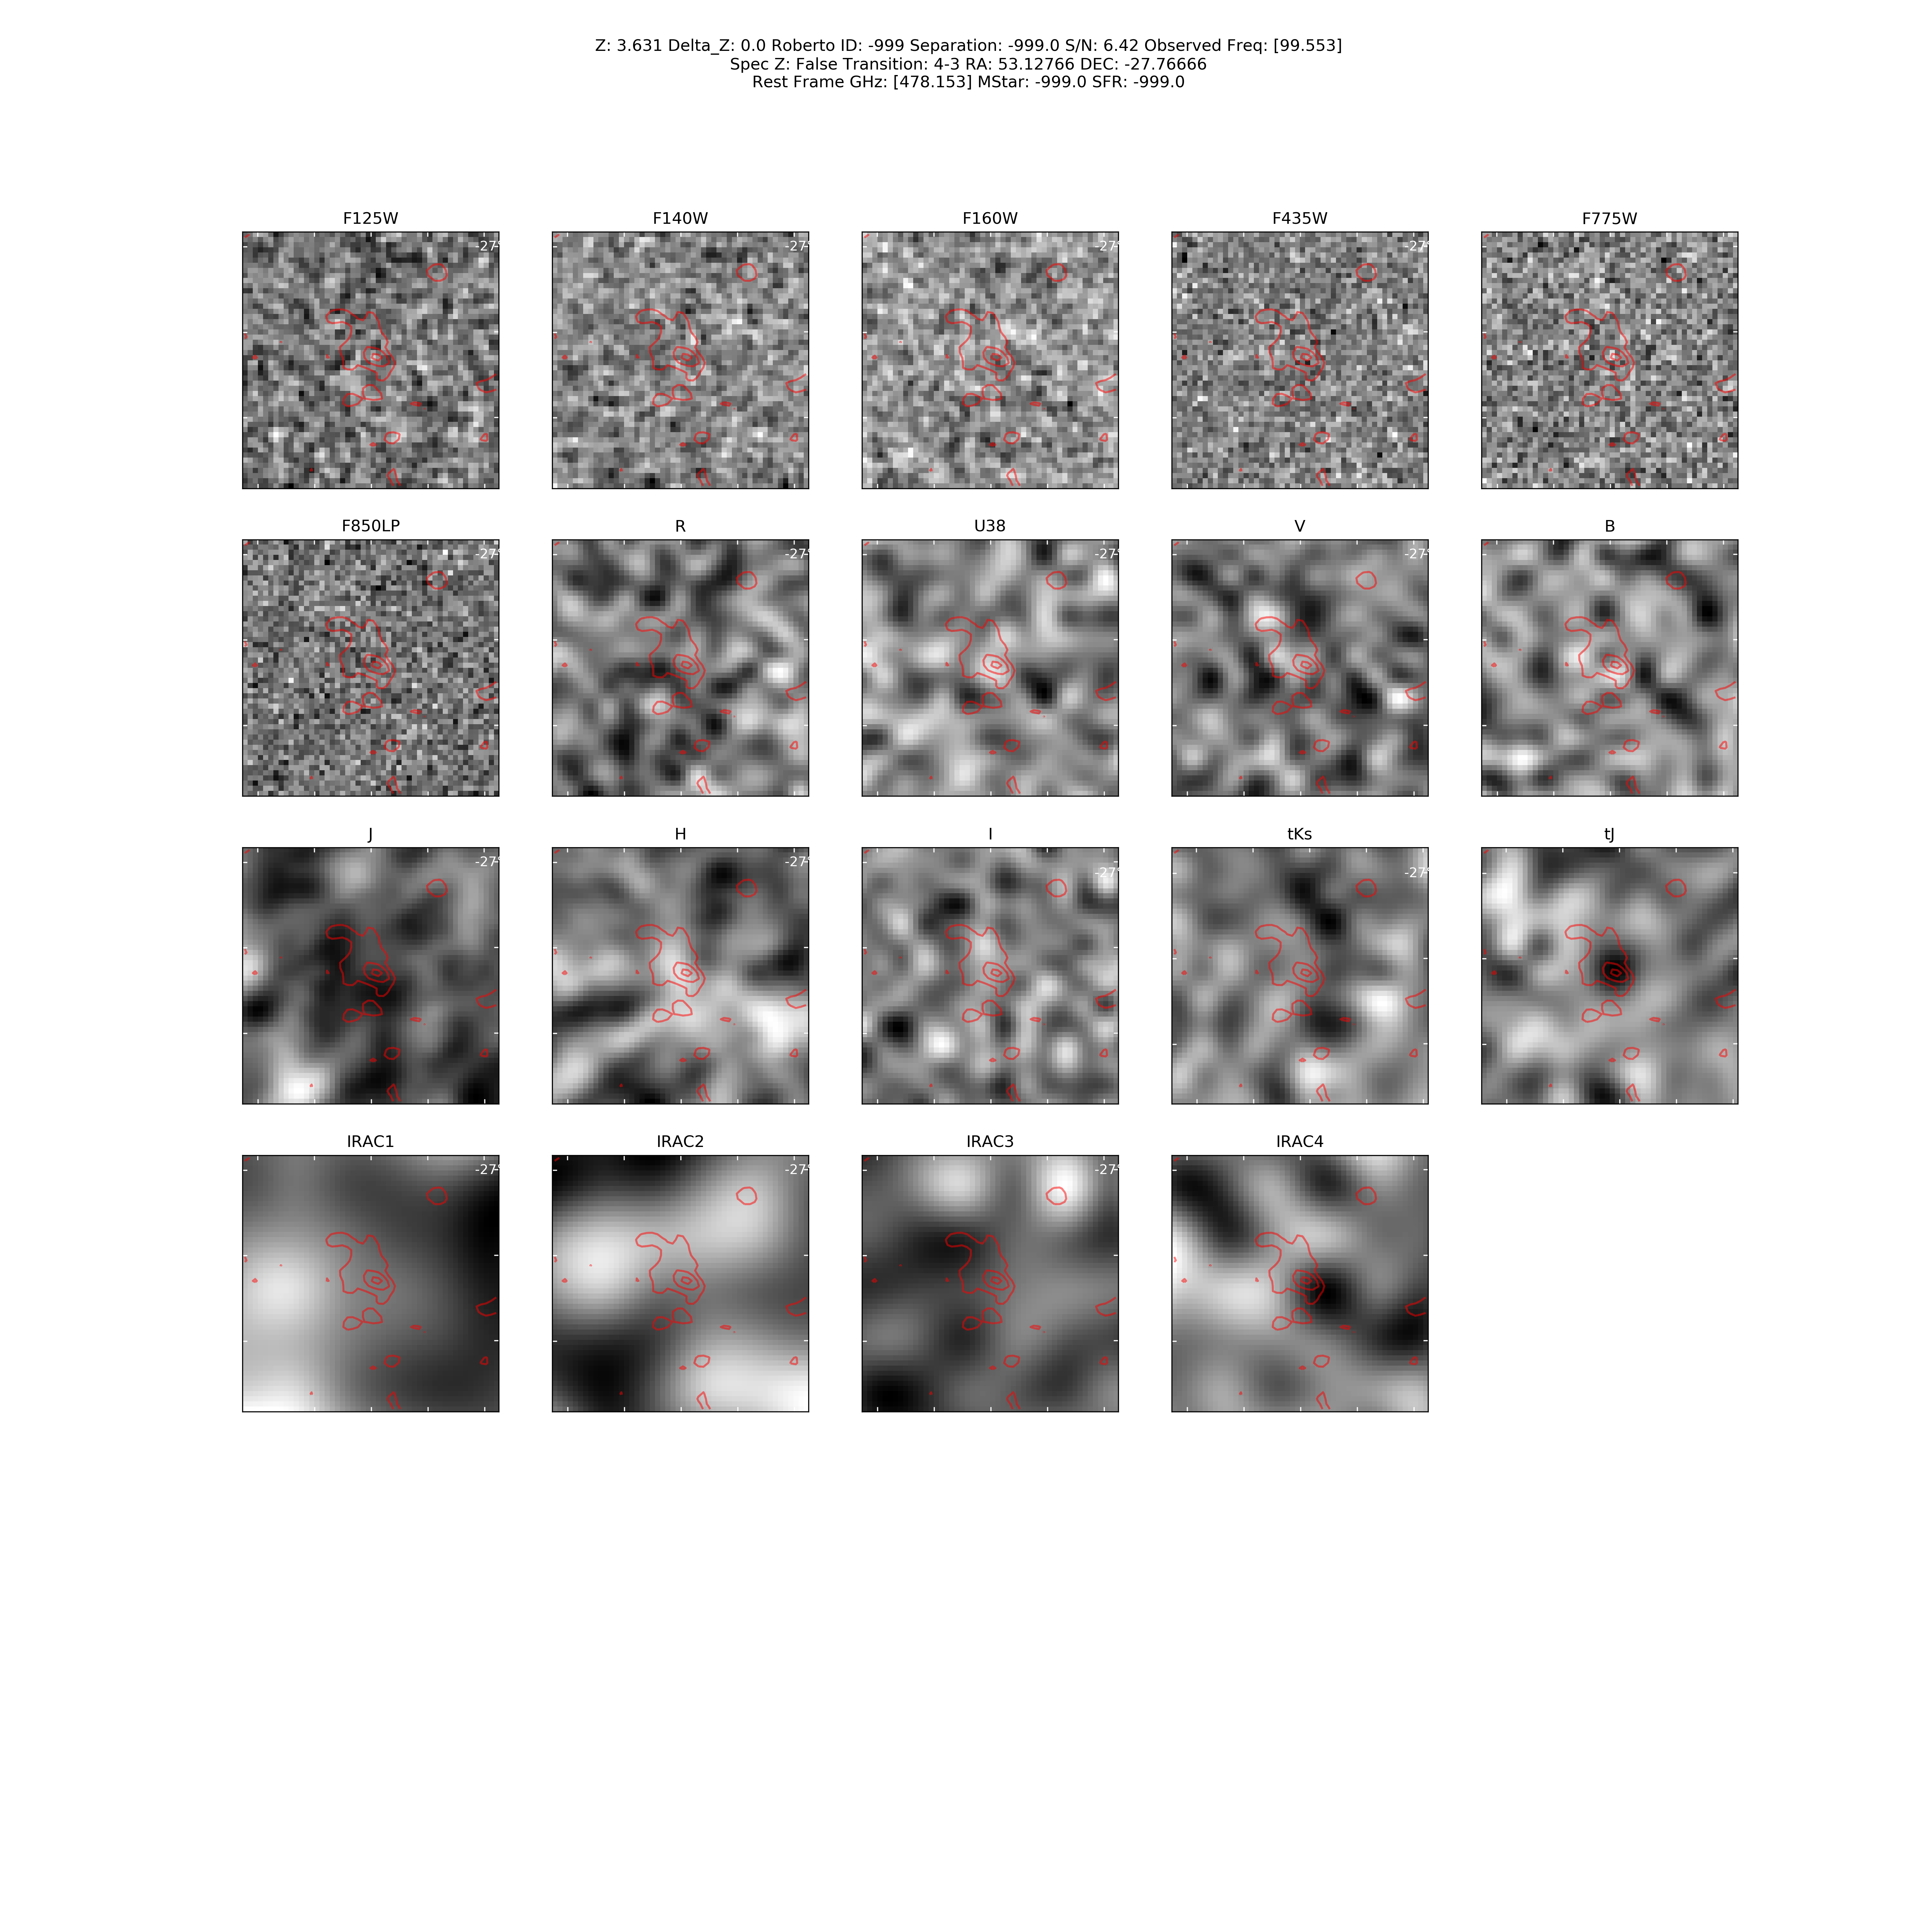
\includegraphics[width=160mm]{Matched/ASPECS_Cutout_22.png}
\caption{ID.23. Same contours and cutout size as for \ref{fig:Match_One}.}
\label{fig:Match_Three}
\end{figure}

\begin{figure}[tbp]
\centering 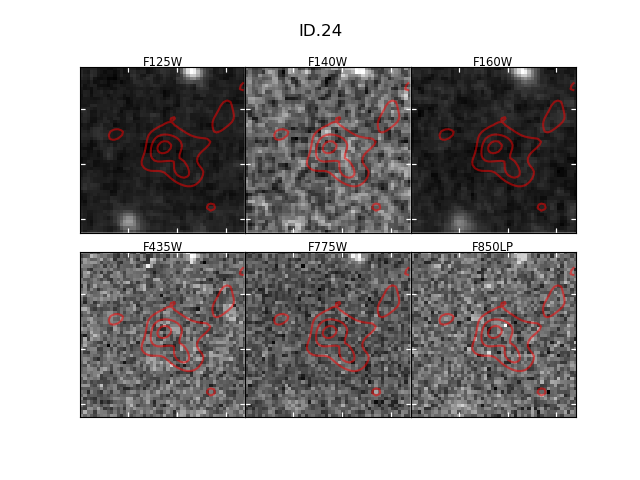
\includegraphics[width=160mm]{Matched/ASPECS_Cutout_23.png}
\caption{ID.24. Same contours and cutout size as for \ref{fig:Match_One}.}
\label{fig:Match_Three}
\end{figure}

\begin{figure}[tbp]
\centering 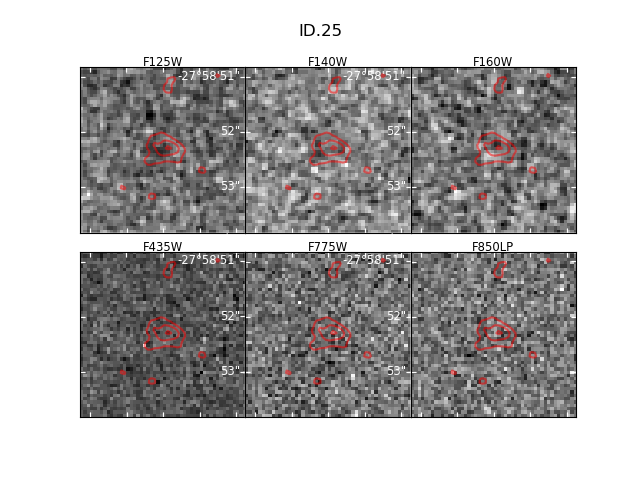
\includegraphics[width=160mm]{Matched/ASPECS_Cutout_24.png}
\caption{ID.25. Same contours and cutout size as for \ref{fig:Match_One}.}
\label{fig:Match_Three}
\end{figure}

\begin{figure}[tbp]
\centering 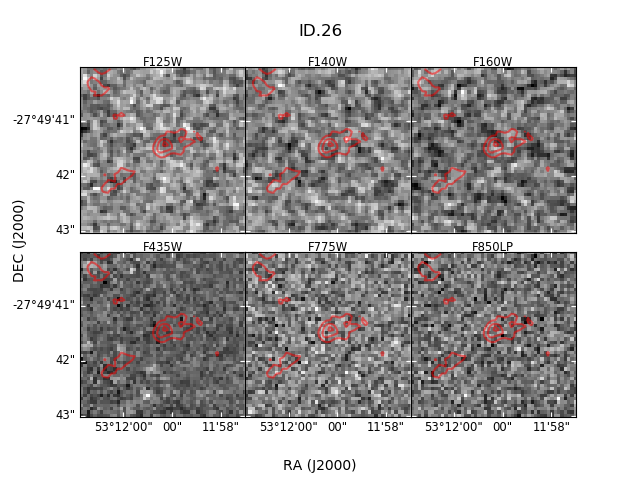
\includegraphics[width=160mm]{Matched/ASPECS_Cutout_25.png}
\caption{ID.26. Same contours and cutout size as for \ref{fig:Match_One}.}
\label{fig:Match_Three}
\end{figure}

\begin{figure}[tbp]
\centering 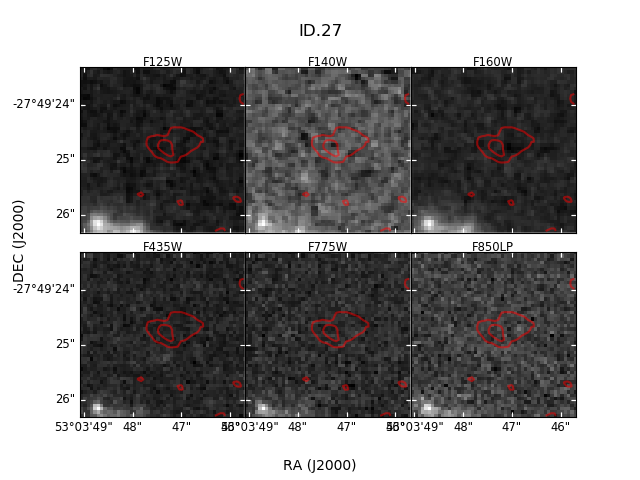
\includegraphics[width=160mm]{Matched/ASPECS_Cutout_26.png}
\caption{ID.27. Same contours and cutout size as for \ref{fig:Match_One}.}
\label{fig:Match_Three}
\end{figure}

\begin{figure}[tbp]
\centering 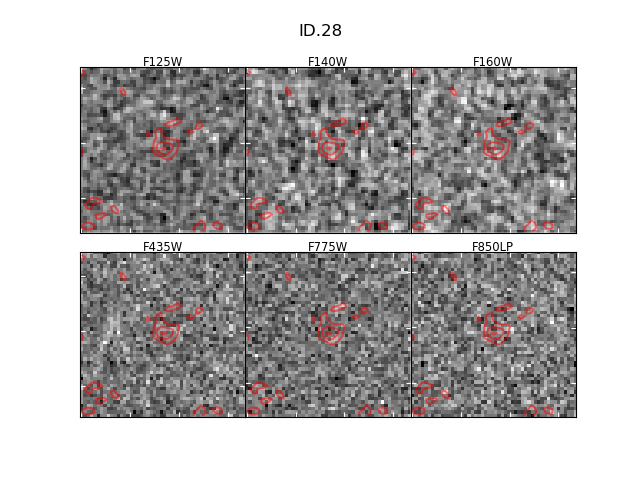
\includegraphics[width=160mm]{Matched/ASPECS_Cutout_27.png}
\caption{ID.28. Same contours and cutout size as for \ref{fig:Match_One}.}
\label{fig:Match_Three}
\end{figure}

\begin{figure}[tbp]
\centering 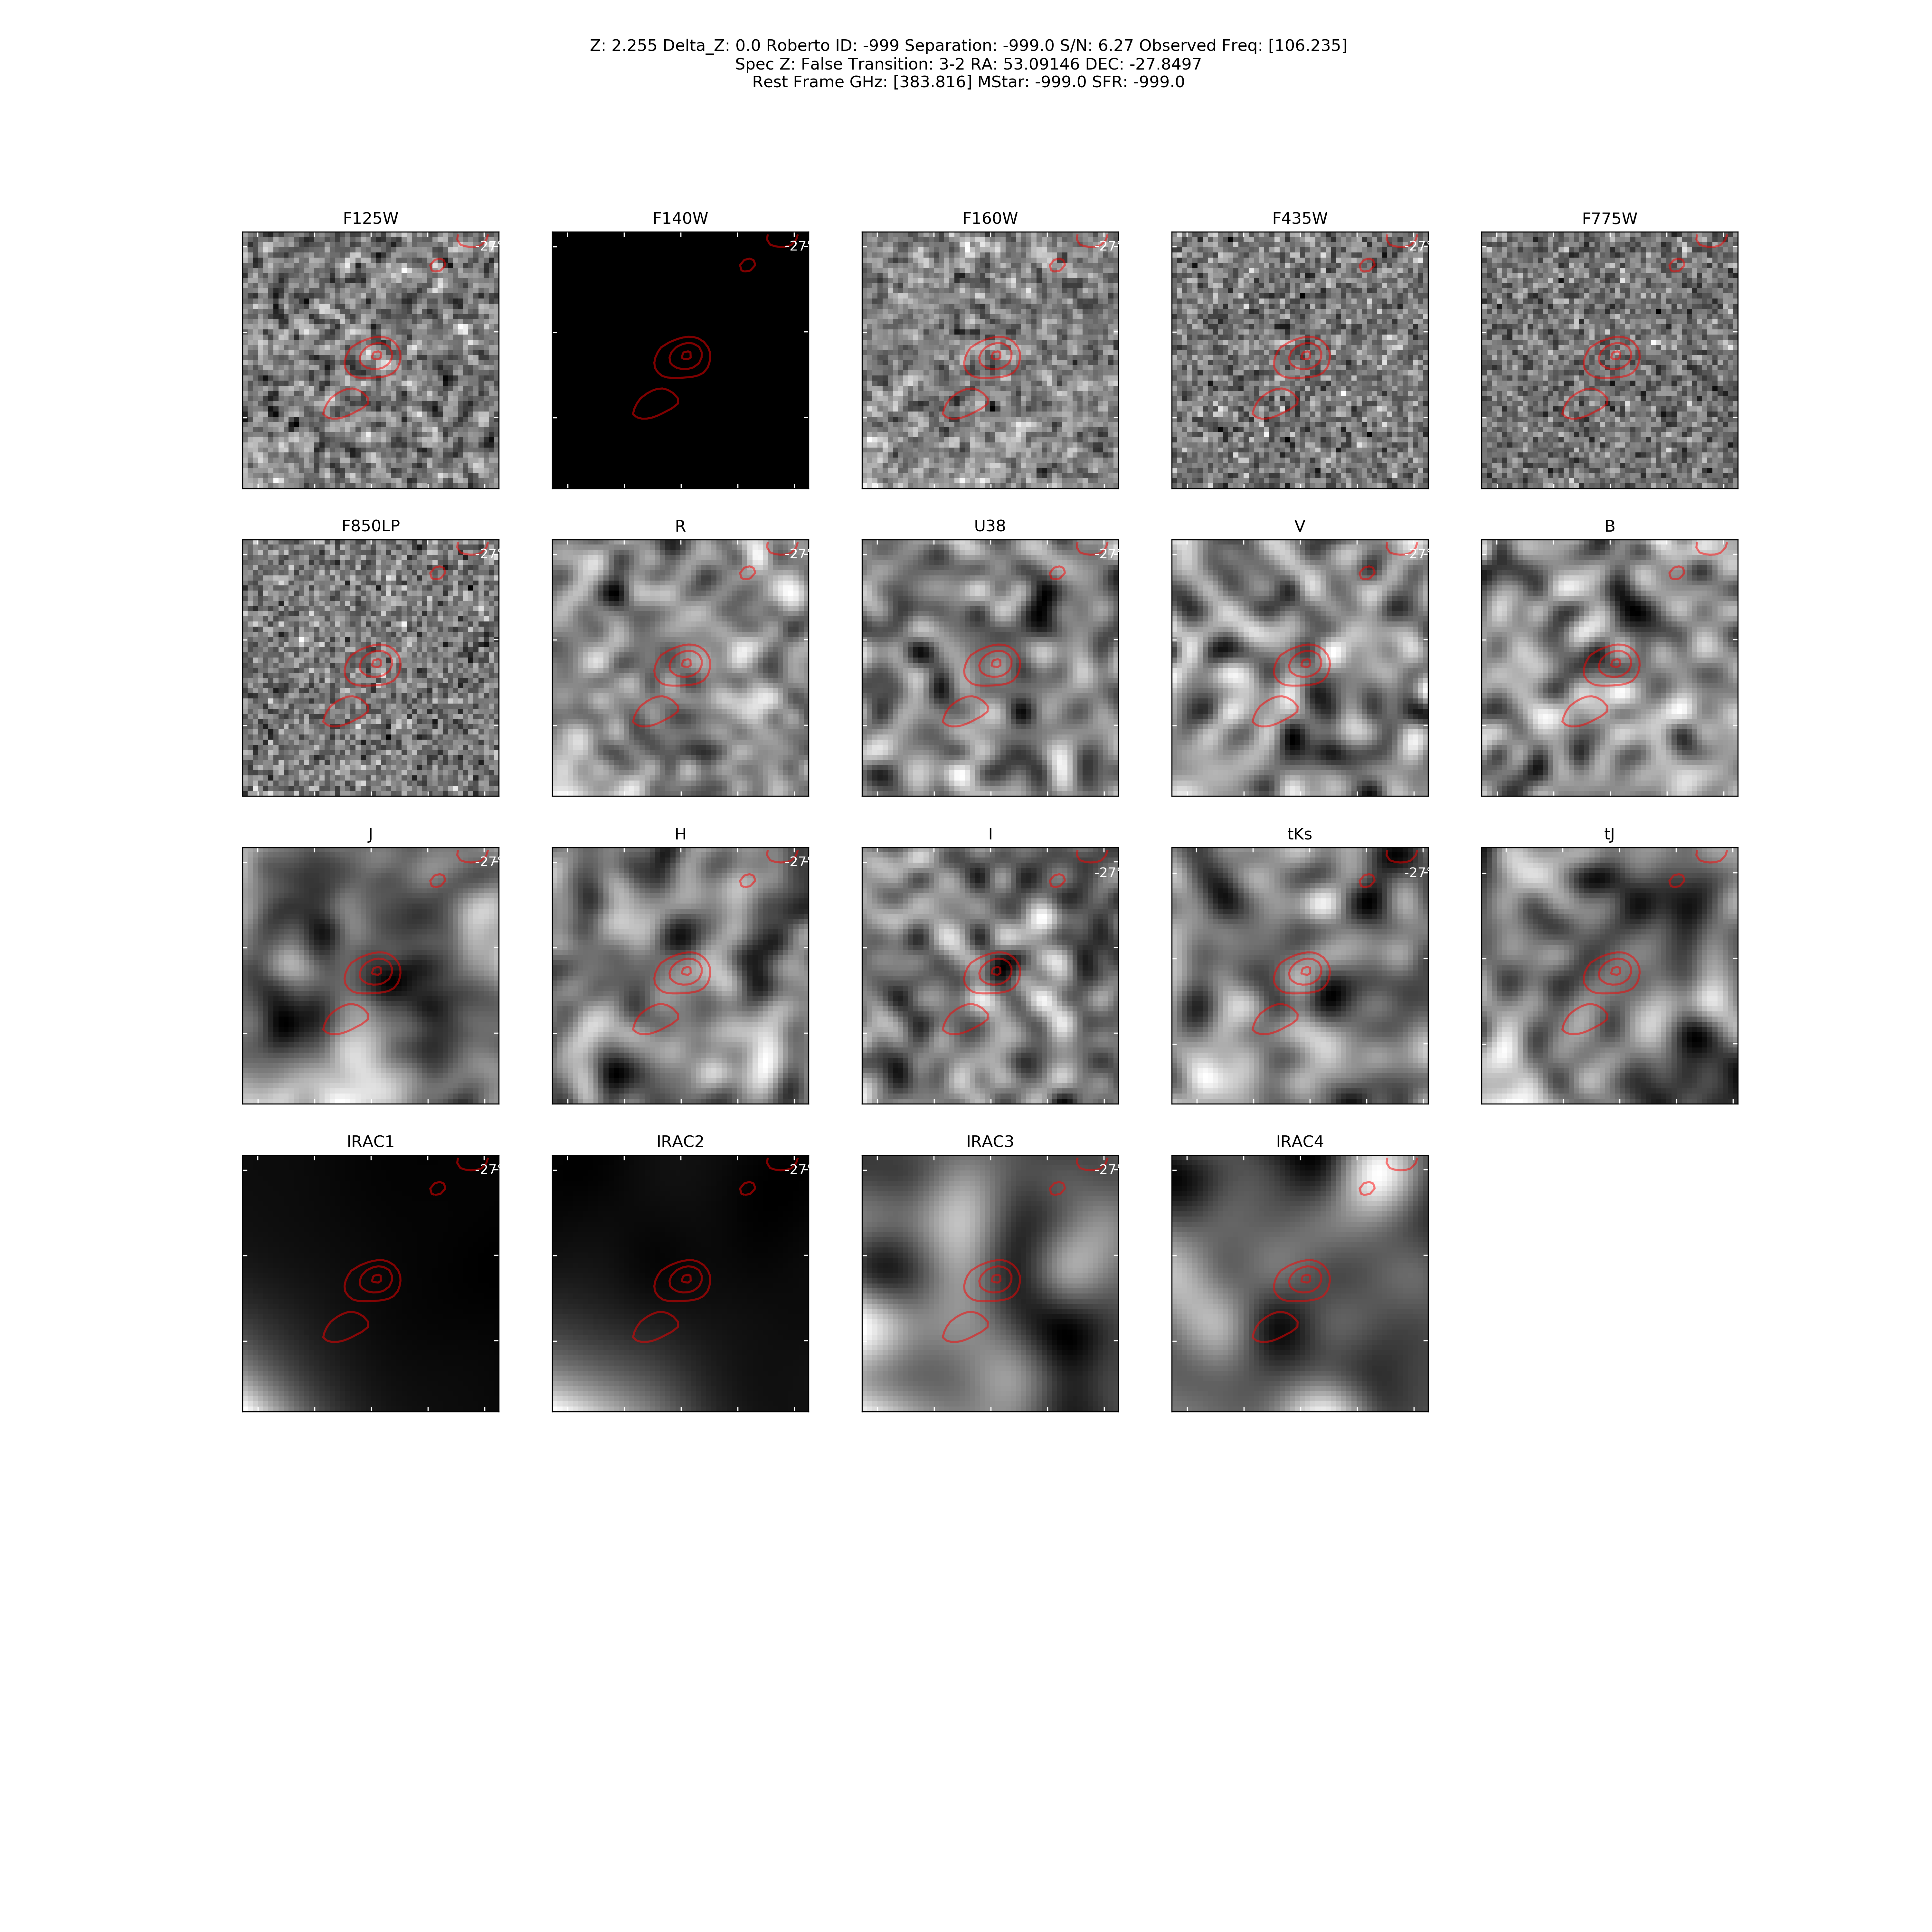
\includegraphics[width=160mm]{Matched/ASPECS_Cutout_28.png}
\caption{ID.29. Same contours and cutout size as for \ref{fig:Match_One}.}
\label{fig:Match_Three}
\end{figure}

\begin{figure}[tbp]
\centering 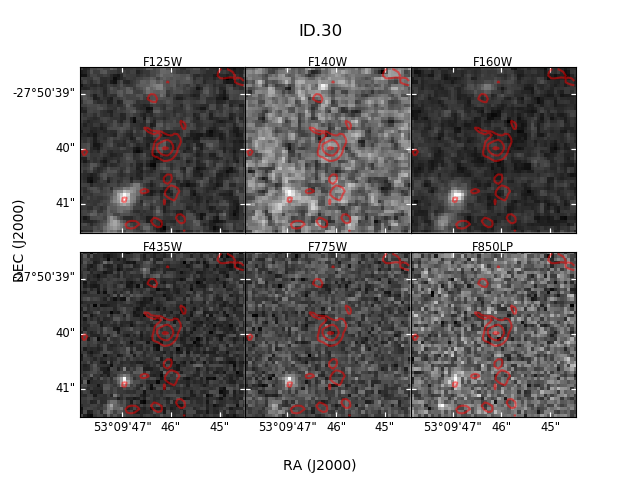
\includegraphics[width=160mm]{Matched/ASPECS_Cutout_29.png}
\caption{ID.30. Same contours and cutout size as for \ref{fig:Match_One}.}
\label{fig:Match_Three}
\end{figure}

\begin{figure}[tbp]
\centering 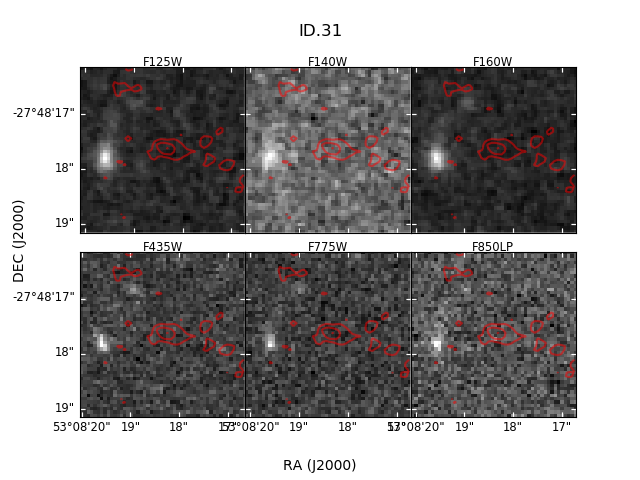
\includegraphics[width=160mm]{Matched/ASPECS_Cutout_30.png}
\caption{ID.31. Same contours and cutout size as for \ref{fig:Match_One}.}
\label{fig:Match_Three}
\end{figure}

\begin{figure}[tbp]
\centering 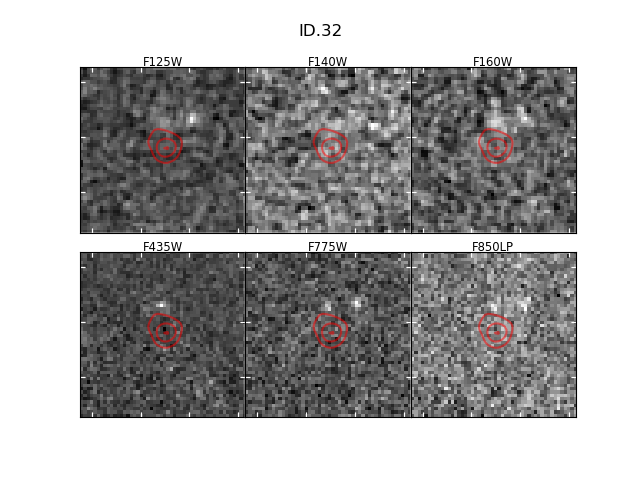
\includegraphics[width=160mm]{Matched/ASPECS_Cutout_31.png}
\caption{ID.32. Same contours and cutout size as for \ref{fig:Match_One}.}
\label{fig:Match_Three}
\end{figure}

\begin{figure}[tbp]
\centering 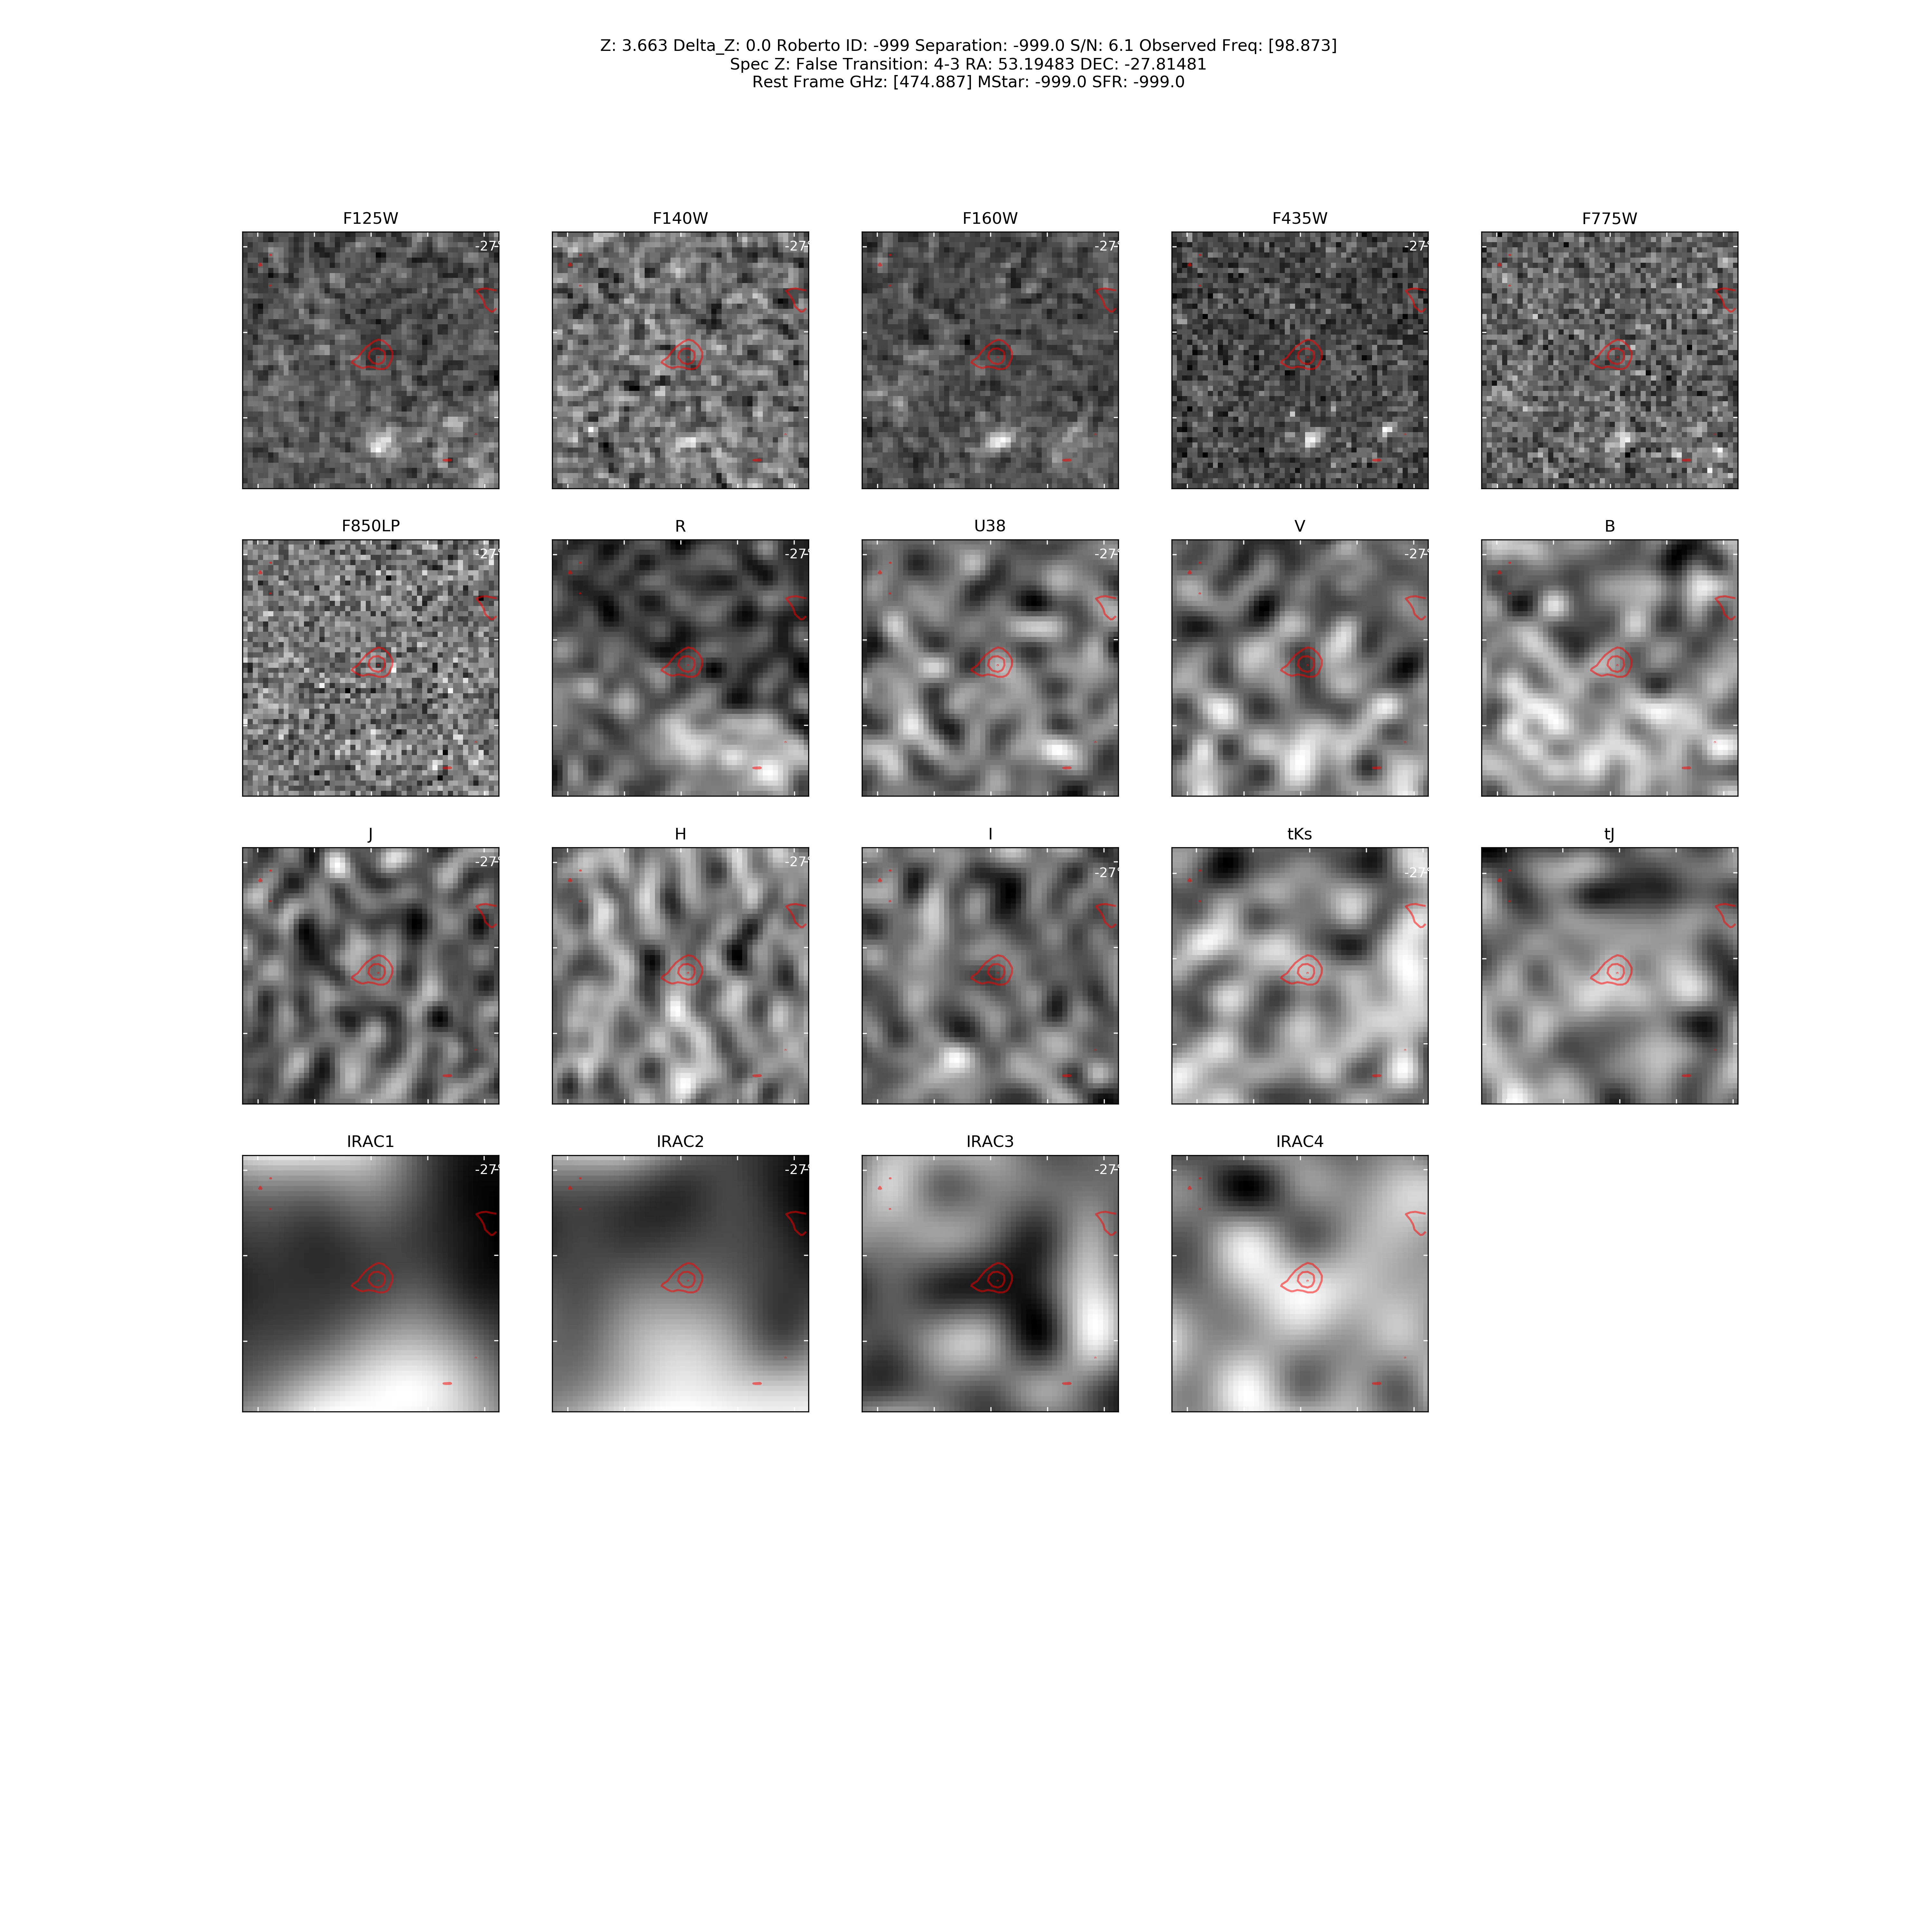
\includegraphics[width=160mm]{Matched/ASPECS_Cutout_32.png}
\caption{ID.33. Same contours and cutout size as for \ref{fig:Match_One}.}
\label{fig:Match_Three}
\end{figure}

\begin{figure}[tbp]
\centering \includegraphics[width=160mm]{Matched/ASPECS_Cutout_33.png}
\caption{ID.34. Same contours and cutout size as for \ref{fig:Match_One}.}
\label{fig:Match_Three}
\end{figure}

\begin{figure}[tbp]
\centering \includegraphics[width=160mm]{Matched/ASPECS_Cutout_34.png}
\caption{ID.35. Same contours and cutout size as for \ref{fig:Match_One}.}
\label{fig:Match_Three}
\end{figure}


\bibliographystyle{unsrt}
\bibliography{refs}

\end{document}
